\documentclass [10pt]{article}
\usepackage[a4paper, inner=3cm, outer=3cm, top=2cm, bottom=3cm, bindingoffset=0.5cm]{geometry}
\usepackage[english]{babel} % localization and internationalization
\usepackage{blindtext}
\usepackage{graphicx}
\usepackage{parskip} % for paragraph spacing
\usepackage{xcolor} % increases range of colours available
\usepackage{colortbl}
\usepackage{tcolorbox} % for coloured quotation pulls
\usepackage{tabularx}
\usepackage{booktabs}
\usepackage{enumitem}
\usepackage[colorlinks=true, linkcolor=blue, citecolor=green, urlcolor=macsblue]{hyperref} % to enable and colour hyperlinks urlcolor was cyan
% \usepackage[colorlinks=true, linkcolor=red, urlcolor=blue]{hyperref}
\usepackage{wrapfig} % to layout images etc.
\usepackage[normalem]{ulem}
\usepackage{paralist}  % for list and enum formatting
\usepackage{caption}
\usepackage{url}
\usepackage[autostyle]{csquotes} % for correct quotation marks
\usepackage{amsmath}
\usepackage{placeins}
\usepackage{float} % To help with image placement


\newtcolorbox{faintquote}{ colback=blue!15, colframe=blue!50, boxrule=1pt, arc=2mm, left=4mm, right=4mm }
\newtcolorbox{advisory}{ colback=red!15, colframe=red!50, boxrule=1pt, arc=2mm, left=4mm, right=4mm }
\newtcolorbox{learnpoint}{ colback=green!15, colframe=green!50, boxrule=1pt, arc=2mm, left=4mm, right=4mm }
\definecolor{commentGreen}{RGB}{48,110,30}
\definecolor{macsblue}{RGB}{0,12,123}

\setlength{\plitemsep}{3pt}

\newcommand{\collaborators}[1]{\par\small\textbf{Technical Advisors:\\} #1}
\newcommand{\soundfiles}[1]{\par\small\textbf{Sound Files By:\\} #1}
\newcommand{\review}[1]{\par\small\textbf{Reviewers:\\} #1}

\hypersetup{pdftitle={MACS - MNW Acoustic Classification Suite}}

% \pagestyle{empty}

\title{MACS - MNW Acoustic Classification Suite (v0.2.5)}
\author{Nick Bowling (@Skittles)}
\date{\today}

\begin{document}
\maketitle
\collaborators{@mahzel\\ @snrkatat}
\soundfiles{@snrkatat\\ @Skittles\\ @Johns}
% \review{@Mahzel, @snrkatat, @Johns, \verb|@Doctor_Dystopia|, \verb|@Pgen_FFW36|, @PLOP, @MasterGunner309}
\review{@Mahzel\\ @snrkatat\\ @Johns\\ @Doctor\_Dystopia\\ @Pgen\_FFW36\\ @PLOP\\ @MasterGunner309} \\

{\centering
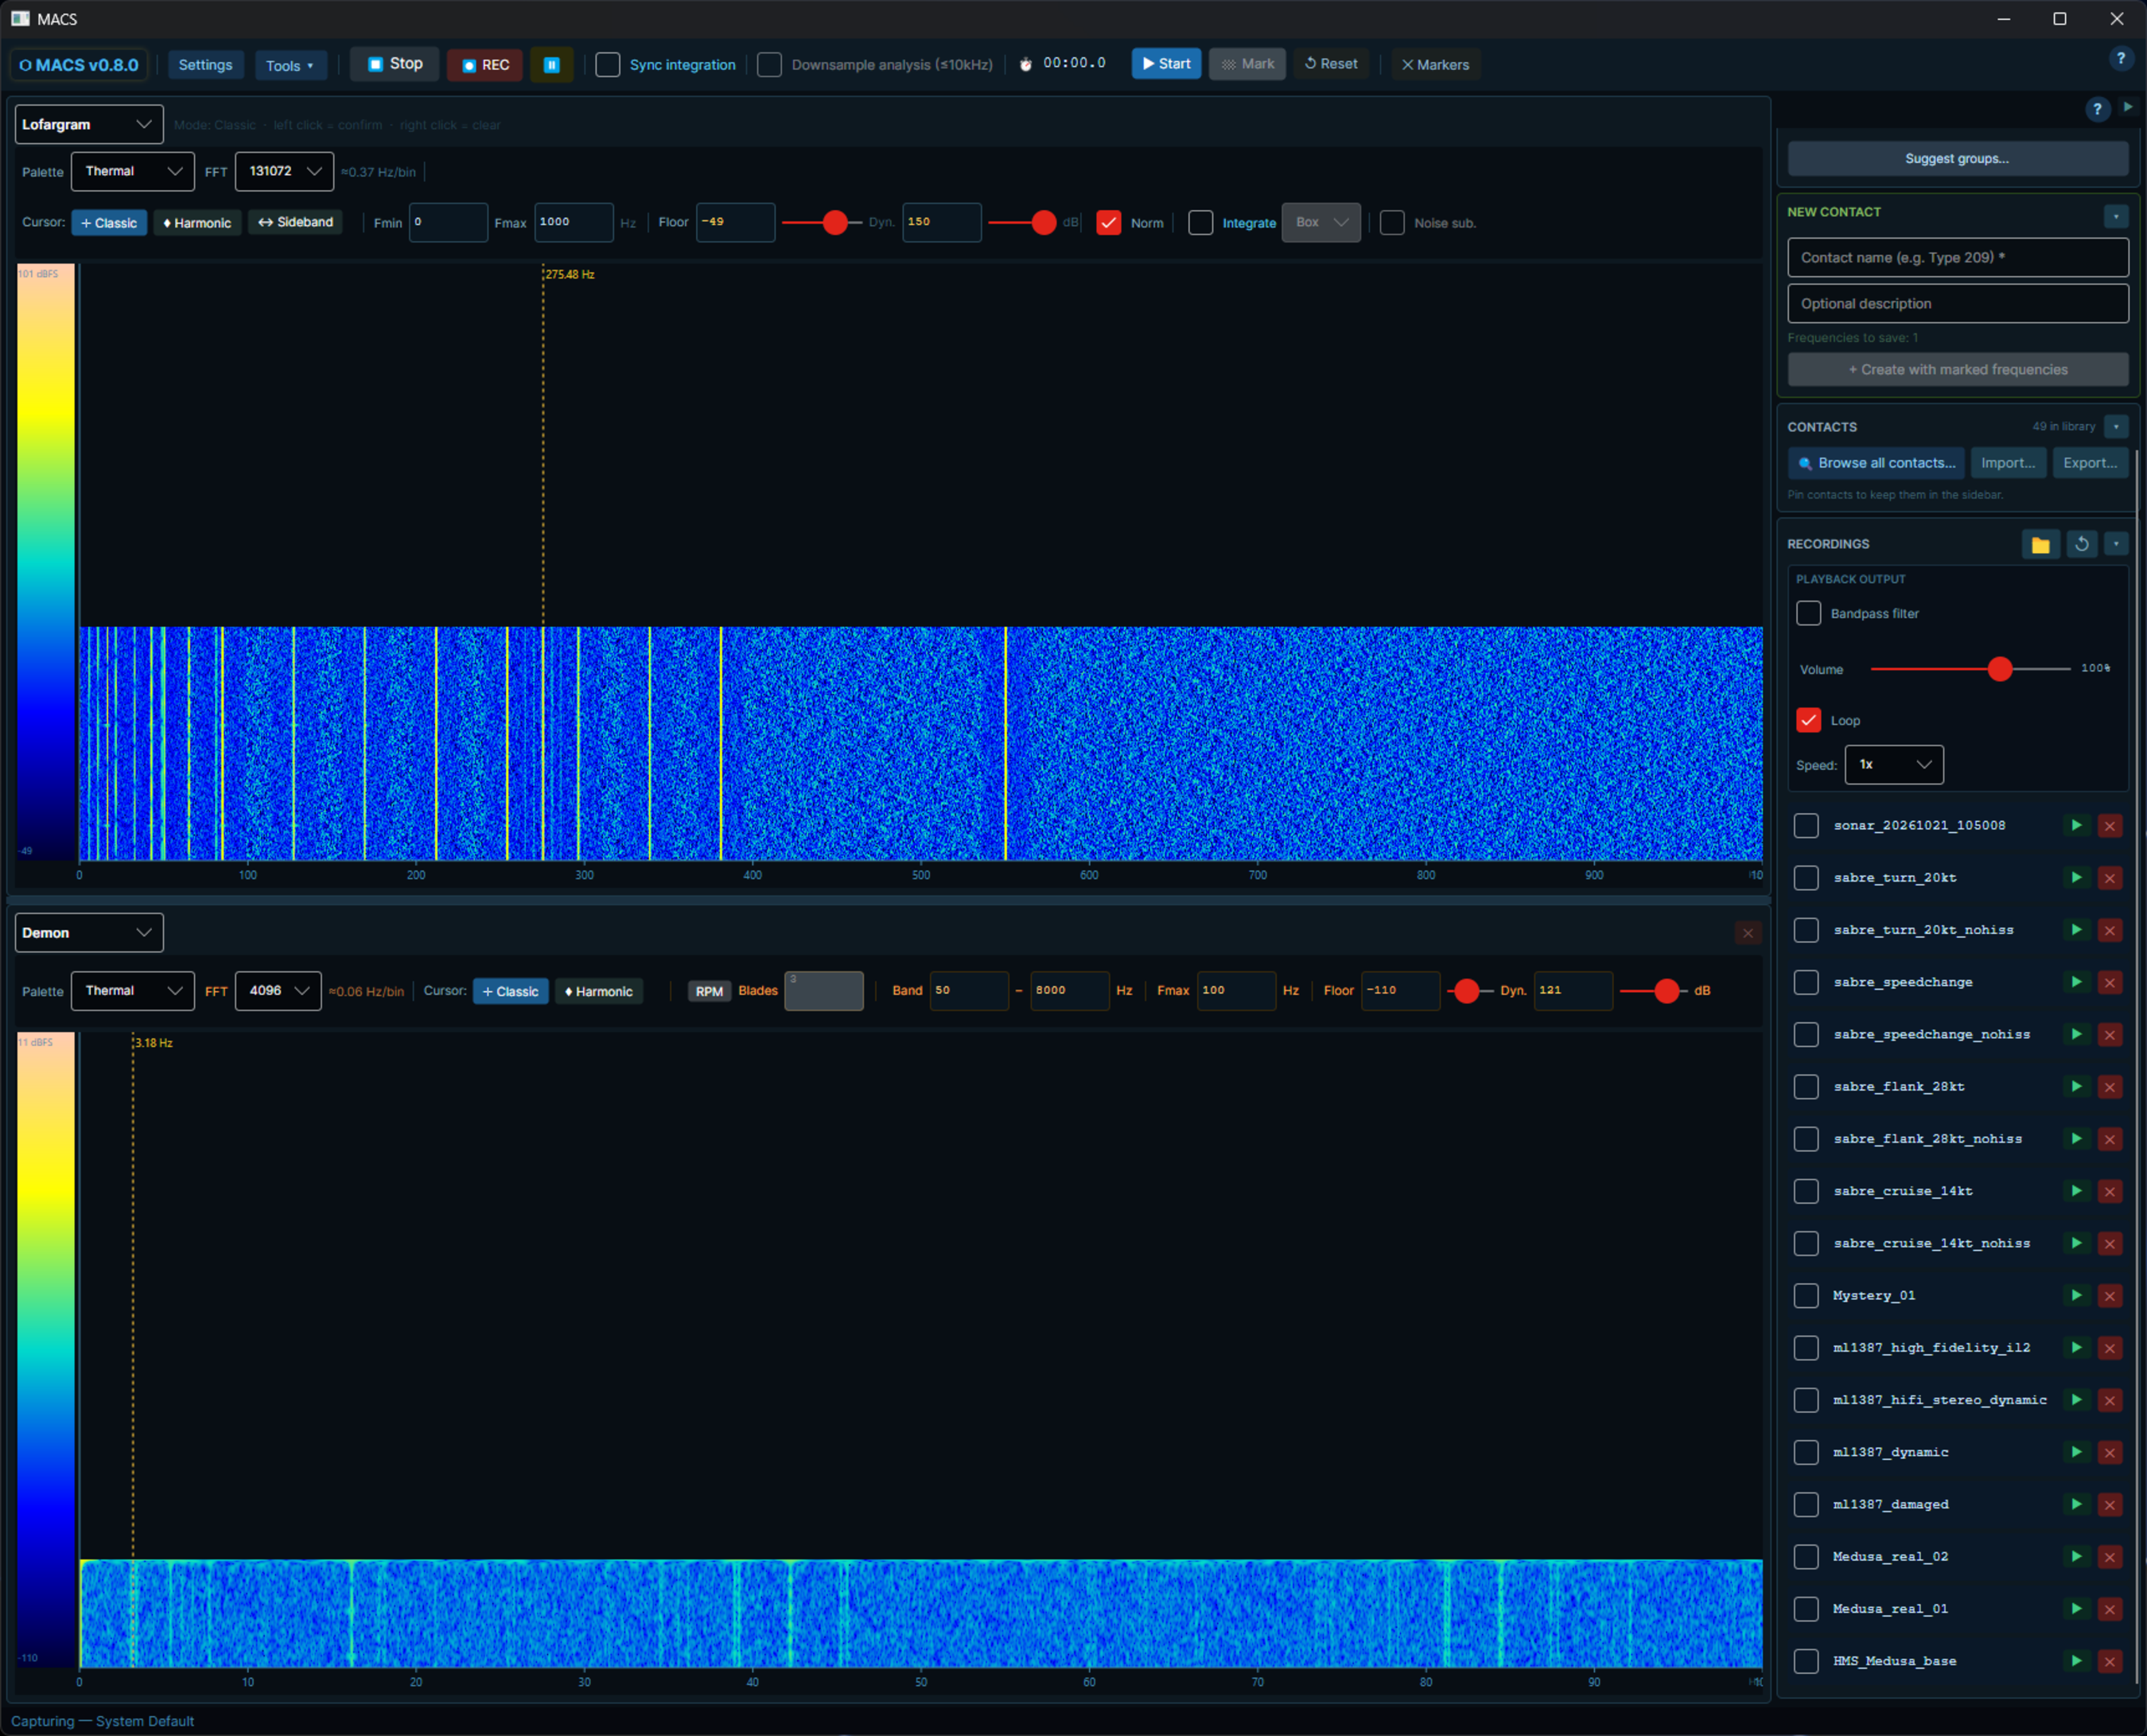
\includegraphics[width=400px]{../img/actuals/Cover.pdf}
\par}

\newpage
{
\setcounter{tocdepth}{3}
\tableofcontents
}

\begin{advisory}
    This document is still under active development as @Mahzel adds exciting new features and improves existing ones. This means that inevitably this guide will lag behind the currently available version of MACS. This is not necessarily a problem as this guide is primarily aimed at new users looking to enhance their experience of playing Modern Naval Warfare. New users are unlikely to be concerned with the more advanced capabilities of MACS.\\
    \\ \textbf{This guide is a community document so the team that has produced it welcome feedback and suggestions via the two MNW Discord channels. Updates to this document will be announced there as well.}
\end{advisory}

\newpage


\section{Overview}
\textbf{Note for new users.} If you are unfamiliar with sound analysis, SONAR, and the mathematics behind it I strongly recommend that you read the friendly guides in \hyperref[sec:Appendix_A]{Appendix A} and the relevant chapter in the \href{https://docs.waveops.io/mnw/mnw-guide.pdf}{MNW guide}. You do not need to be a maths wizard to use MACS, but a basic knowledge of the concepts will help you understand what is going on. If you enjoy the detail then \hyperref[sec:Appendix_B]{Appendix B} goes deeper into the concepts. In Mahzel's own words:

\begin{faintquote}
	MACS is a tool provided as an advanced suite for enthusiasts of acoustic analysis. It also provides a custom user-build database where you can slowly build your measurements history, along with all your comments about an encounter. Only had a few seconds of contact? No worries just record it and replay the contact for further analysis for as long as you wish. It includes a database matcher, where you can see if a current contact's markings correspond to something in the database. You may have numerous matches, but in the end, you are in charge of the sonar.
\end{faintquote}

\textbf{Download} MACS for Widows, Linux and MacOS from \href{https://github.com/Mahzel/MACS}{here}.

\subsection{Capabilities}
MACS is an acoustic classification tool designed for use with the naval simulation Modern Naval Warfare (MNW) developed by The Maslas Bros and published by Matrix / Slitherine. MACS does not replace the in game tools.

\textbf{MACS features include:}

\begin{compactitem}
	\item Accepting sound input directly from the PC's sound card or other system capability.
	\item Running alongside MNW without significantly impacting performance.
	\item Fine control of several input and output parameters.
	\item Detailed, fine grain multicolour representations of the analysed sound.
	\item Normalization and noise suppression to manage the impact of background noise.
	\item Allowing recording and replay of sounds for future analysis.
	\item A user-managed database of contacts and measurements (a pre-populated downloadable database is available at the MACS website).
	\item A built in matcher to compare current contacts with those in the database.
\end{compactitem}

\subsection{What MACS does and why would I need it?}

MACS provides six complementary signal-processing views to help you identify and characterise surface or submarine contacts by their acoustic signature. The underlying processing is grounded in real passive sonar digital signal analysis: 

\begin{compactitem}
	\item FFT based spectrograms (LOFARgrams).
	\item DEMON envelope detection (DEMONgrams).
	\item Real cepstrum analysis.
	\item Auto correlation.
	\item Power Spectral Density (PSD) analysis.
	\item ZoomFFT analysis.
\end{compactitem}

Explanations of these and how to use them are described in the following sections. Each processing technique provides a different view of the same signal, when used together they can provide a clearer picture of what is happening around you. The more information you have, the better your chances of detecting and classifying a contact.

\textbf{MACS supplements, it does not replace the in-game tools}
\pagebreak
\section{Installing and Configuring MACS}

Currently the MACS application is a stand alone program there is no specific installer. The following describes installation for Windows (11), OSx-x64, OSx-ARM and Linux.

\subsection{Windows.}

\begin{compactenum}
    \item Download the current version from \href{https://github.com/Mahzel/MACS/releases}{\texttt{https://github.com/Mahzel/MACS/releases}}
    \item Copy the downloaded compressed file to a location of your choice, e.g. \path{C:\MACS*.rar}. Where * is current version and OS type suffix, e.g. \enquote{.v0.5.1.win-x64}
    \item Extract the compressed files, Windows' own tools can handle tar compressed files. Right click the file and select extract all, accept defaults which will create a folder called MACS* (where * is version and OS)
    \item Navigate into the extracted folder and again into the folder called win-x64
    \item This step is important. Scroll down until you see the MACS.exe item and \textbf{right click} on it. Select \enquote{Properties} and towards the bottom tick the \enquote{Unblock} option. Unless you have changed the default settings windows blocks downloaded .exe files by default to protect users.
    \item You can now run the application by clicking on the MACS.exe file
    \item \textbf{Optionally create a shortcut.} At the location for the shortcut (e.g. Desktop) right click $\rightarrow$ New $\rightarrow$ Shortcut. Enter the path to the application e.g. \path{C:\MACS.v0.5.1.win-x64\win-x64\MACS.exe} or wherever you extracted it. Name the shortcut and select Finish.
\end{compactenum}

\subsection{Installing MACS on the Apple MAC OSx-64 and OSx-ARM}

\textbf{Prerequisites}

\begin{compactenum}
    \item User must have Administrator access to the computer and sudo rights, i.e. have an administrator account.
    \item User should determine the type of CPU their machine to ensure correct MACS version is installed.
    \item User will need to install a .rar file unarchiver such as “The Unarchiver” from the App store (free) if a suitable app is not already installed.
\end{compactenum}

\textbf{To determine the type of CPU}

Method 1: Using “About This Mac” (GUI)

\begin{compactenum}
    \item Click the Apple logo in the top-left corner of your screen.
    \item Select About This Mac.
    \item Look at the processor description:
    \begin{compactitem}
        \item Apple Silicon (ARM): You will see an entry labelled Chip (e.g., Apple M1, M2, M3, etc.). Or
        \item Intel (x64): You will see an entry labelled Processor (e.g., Intel Core i7).
    \end{compactitem}
\end{compactenum}

Method 2: Using the Terminal

If you prefer using the command line:

\begin{compactenum}
    \item Open the Terminal app (search for it in Spotlight or find it in Applications > Utilities).
    \item Type the following at the command prompt and press Enter: uname -m
    \item Check the output:
    \begin{compactitem}
        \item arm64: This means your Mac is running on ARM (Apple Silicon).
        \item x86\_64: This means your Mac is running on x64 (Intel).
    \end{compactitem}
\end{compactenum}

\textbf{Download and Extract MACS}

\begin{compactenum}
    \item Download the correct version of MACS from \href{https://github.com/Mahzel/MACS/releases}{\texttt{https://github.com/Mahzel/MACS/releases}}
    \begin{compactitem}
        \item MACSosx-x64.rar for i86-64x CPUs
        \item MACSosx-arm64 for ARM CPUs
    \end{compactitem}
    \item Normally this will download into the Downloads folder
    \item Copy the downloaded file to a directory of your choice, e.g. create a folder with \\
    \texttt{mkdir /Users/yourusername/Apps}
    \begin{compactitem}
        \item Note it may be easier to move the file from Downloads to your new directory, e.g. \texttt{mv /Downloads/MACS*.rar /Apps}
    \end{compactitem}   
    \item Extract the file using your .rar file un-packer and export the files. It should create a directory called MACS. Note the exact way the un-archiver will do this varies depending on type. Make sure you are familiar with the way your un-packer works.
\end{compactenum}

\textbf{Making the binary executable}

Downloaded files are not immediately executable by default.

\begin{compactenum}
    \item Open a Terminal and navigate into the MACS folder, e.g. in Terminal \texttt{cd Apps/MACS/osx-x64} or osx-arm64
    \item Type the following at the command prompt \texttt{chmod +x MACS} this sets the execution flag so that the application can run. Note The OS may require you to run this as an administrator, i.e. \texttt{sudo chmod +x MACS} then enter user password to authenticate.
\end{compactenum}

\textbf{How to remove the quarantine flag recursively}

\begin{faintquote}
    Note Un-quarantining software from dubious sources can be risky do not do this routinely. The MACS software is rigorously checked for malware so it is safe to proceed.
\end{faintquote}

Apple blocks direct execution of downloaded files by quarantining them, un-quarantine them as follows:

\begin{compactenum}
    \item Open the Terminal and type the following command (make sure to include a space after the final -d): \texttt{sudo xattr -r -d com.apple.quarantine}. \textbf{Do not press RETURN yet}
    \item Leave a space after quarantine, then drag and drop the folder from Finder directly into the Terminal window. This will automatically fill in the correct path to the folder. Your command should look similar to this: \texttt{sudo xattr -r -d com.apple.quarantine /Users/yourusername/Apps/MACS}
    \item Press Return/Enter on your keyboard.
    \item If asked enter your Mac's login password (no characters or asterisks will show on screen as you type, which is normal security behaviour) and hit Enter again. You may not be asked if your sudo session from above ius still active.
\end{compactenum}

\textbf{Running MACS}

\begin{compactenum}
    \item Open the Terminal and navigate to where you have saved MACS, e.g \\
    \texttt{cd /Users/yourusername/Apps/MACS/osx-x64} or osx-arm64
    \item Type at the prompt \texttt{./MACS}. The first time may take a some time to run because OSx has to build and link the assemblies in the program. Subsequent starts will be much faster.
    \item MACS starts in its own window
\end{compactenum}

\subsection{Installing and Running MACS on Linux}

\textbf{Applies to generic Linux (tested on Ubuntu / Debian)}

\begin{faintquote}
    Note: Because of the variation in the way Linux users configure their computers it is not possible to cover every possible situation. This guide assumes a standard set up with a \path{~/User/Downloads} folder. The author has successfully tested MACS on WSL 2 on Windows 11. However the installation is complicated and requires downloading extra software particularly for the sound system. Since this installation is such an edge case no further details are given here.
\end{faintquote}

\textbf{Prerequisites}

\begin{compactitem}
    \item User must have Administrator access to the computer and sudo rights, i.e.have an administrator account.
    \item User will need to install a .rar file unarchiver such as unrar from if a suitable app is not already installed.
\end{compactitem}

\textbf{Download and Extract MACS}

\begin{compactenum}
    \item Download the current version from \href{https://github.com/Mahzel/MACS/releases}{\texttt{https://github.com/Mahzel/MACS/releases}}
    \item Ensure you download linux-x64.rar version for Linux
    \item Normally this will download into the Downloads folder
    \item Copy the downloaded file to a directory of your choice, e.g. create a folder with \\
    \texttt{mkdir /Users/yourusername/Apps} then move the .rar file to your new folder with \\
    \texttt{mv /Downloads/MACS*.rar /Apps}
    \item Extract the file using your .rar file un-packer, it should create a directory called MACS. Note the exact way the un-archiver will do this varies depending on type. Make sure you are familiar with the way your un-packer works.
\end{compactenum}

\textbf{Making the binary executable}

Downloaded files are not immediately executable by default.

\begin{compactenum}
    \item Open a Terminal and navigate into the MACS folder, e.g. in Terminal cd Apps/MACS/linux-x64
    \item Type the following at the command prompt \texttt{chmod +x MACS} this sets the execution flag so that the application can run. Note The OS may require you to run this as an administrator, i.e. \texttt{sudo chmod +x MACS} then enter user password to authenticate.
\end{compactenum}

\textbf{Running MACS}

\begin{compactenum}
    \item Open the Terminal and navigate to where you have saved MACS, e.g \\
    \texttt{cd /Users/yourusername/Apps/MACS/linux-x64}
    \item Type at the prompt ./MACS the first time may take a while to run because Linux has to build and link the assemblies in the program. Subsequent starts will be much faster.
    \item MACS starts in its own window
\end{compactenum}

\subsection{Initial Configuring and Basic Settings}

After installation MACS is configured with sensible basic defaults for most settings. Two settings that should be checked are:

\begin{compactitem}
    \item Devices
    \item Recordings Location
\end{compactitem}

\textbf{Devices}
This depends on individual users PCs set up but in most cases defaults will work.

\begin{compactitem}
    \item \textbf{Capture Device} is the device that MACS uses to capture the sound input. In most cases this will be the active sound card in a loopback configuration. In some cases this may be something else such as a microphone.
    \item \textbf{Live Monitor Output Device} The device used to play back the live sound. This must be a separate device to that used for capture or feedback will occur.
    \item \textbf{Recording playback device} Device used to playback recordings. Normally set to default or the same as input device as usually the aim is to analyse the sound in app. However this can be configured to play to another device such as headphones if no immediate analysis is needed and the aim is to assess audio such as propeller passes etc.
\end{compactitem}

\textbf{Recordings Location}. Out of the box this is set up by the application on first run. For Windows the default is \path{Documents}. This is generally fine but there are some circumstances where you may want to change this. The most common case is if you are using OneDrive and it is auto-synchronizing. The recordings .wav files can be large and take a long time to upload and take up valuable storage space. Change the location of recordings storage from the Settings $\rightarrow$ General tab. Browse to the location you want to use and select folder in the normal way. This will change the recordings storage to the new location.

For OSx and Linux I currently recommend leaving the default location as it is.

\textbf{Other settings} are configured in a .json file. If the user changes something in the settings panel this file is updated. The .json file is located in different places depending on the operating system. Further details about this file and restoring defaults are given in the  Application Interface - Settings Persistence section.

\pagebreak
\section{Application Interface}

\subsection{Overview}
The application window, Figure 1, is divided into a tool bar and two main regions: a central analysis area with two panels A and B, and a right sidebar with the database and recordings management tools.

\begin{figure}[h]
	\centering
	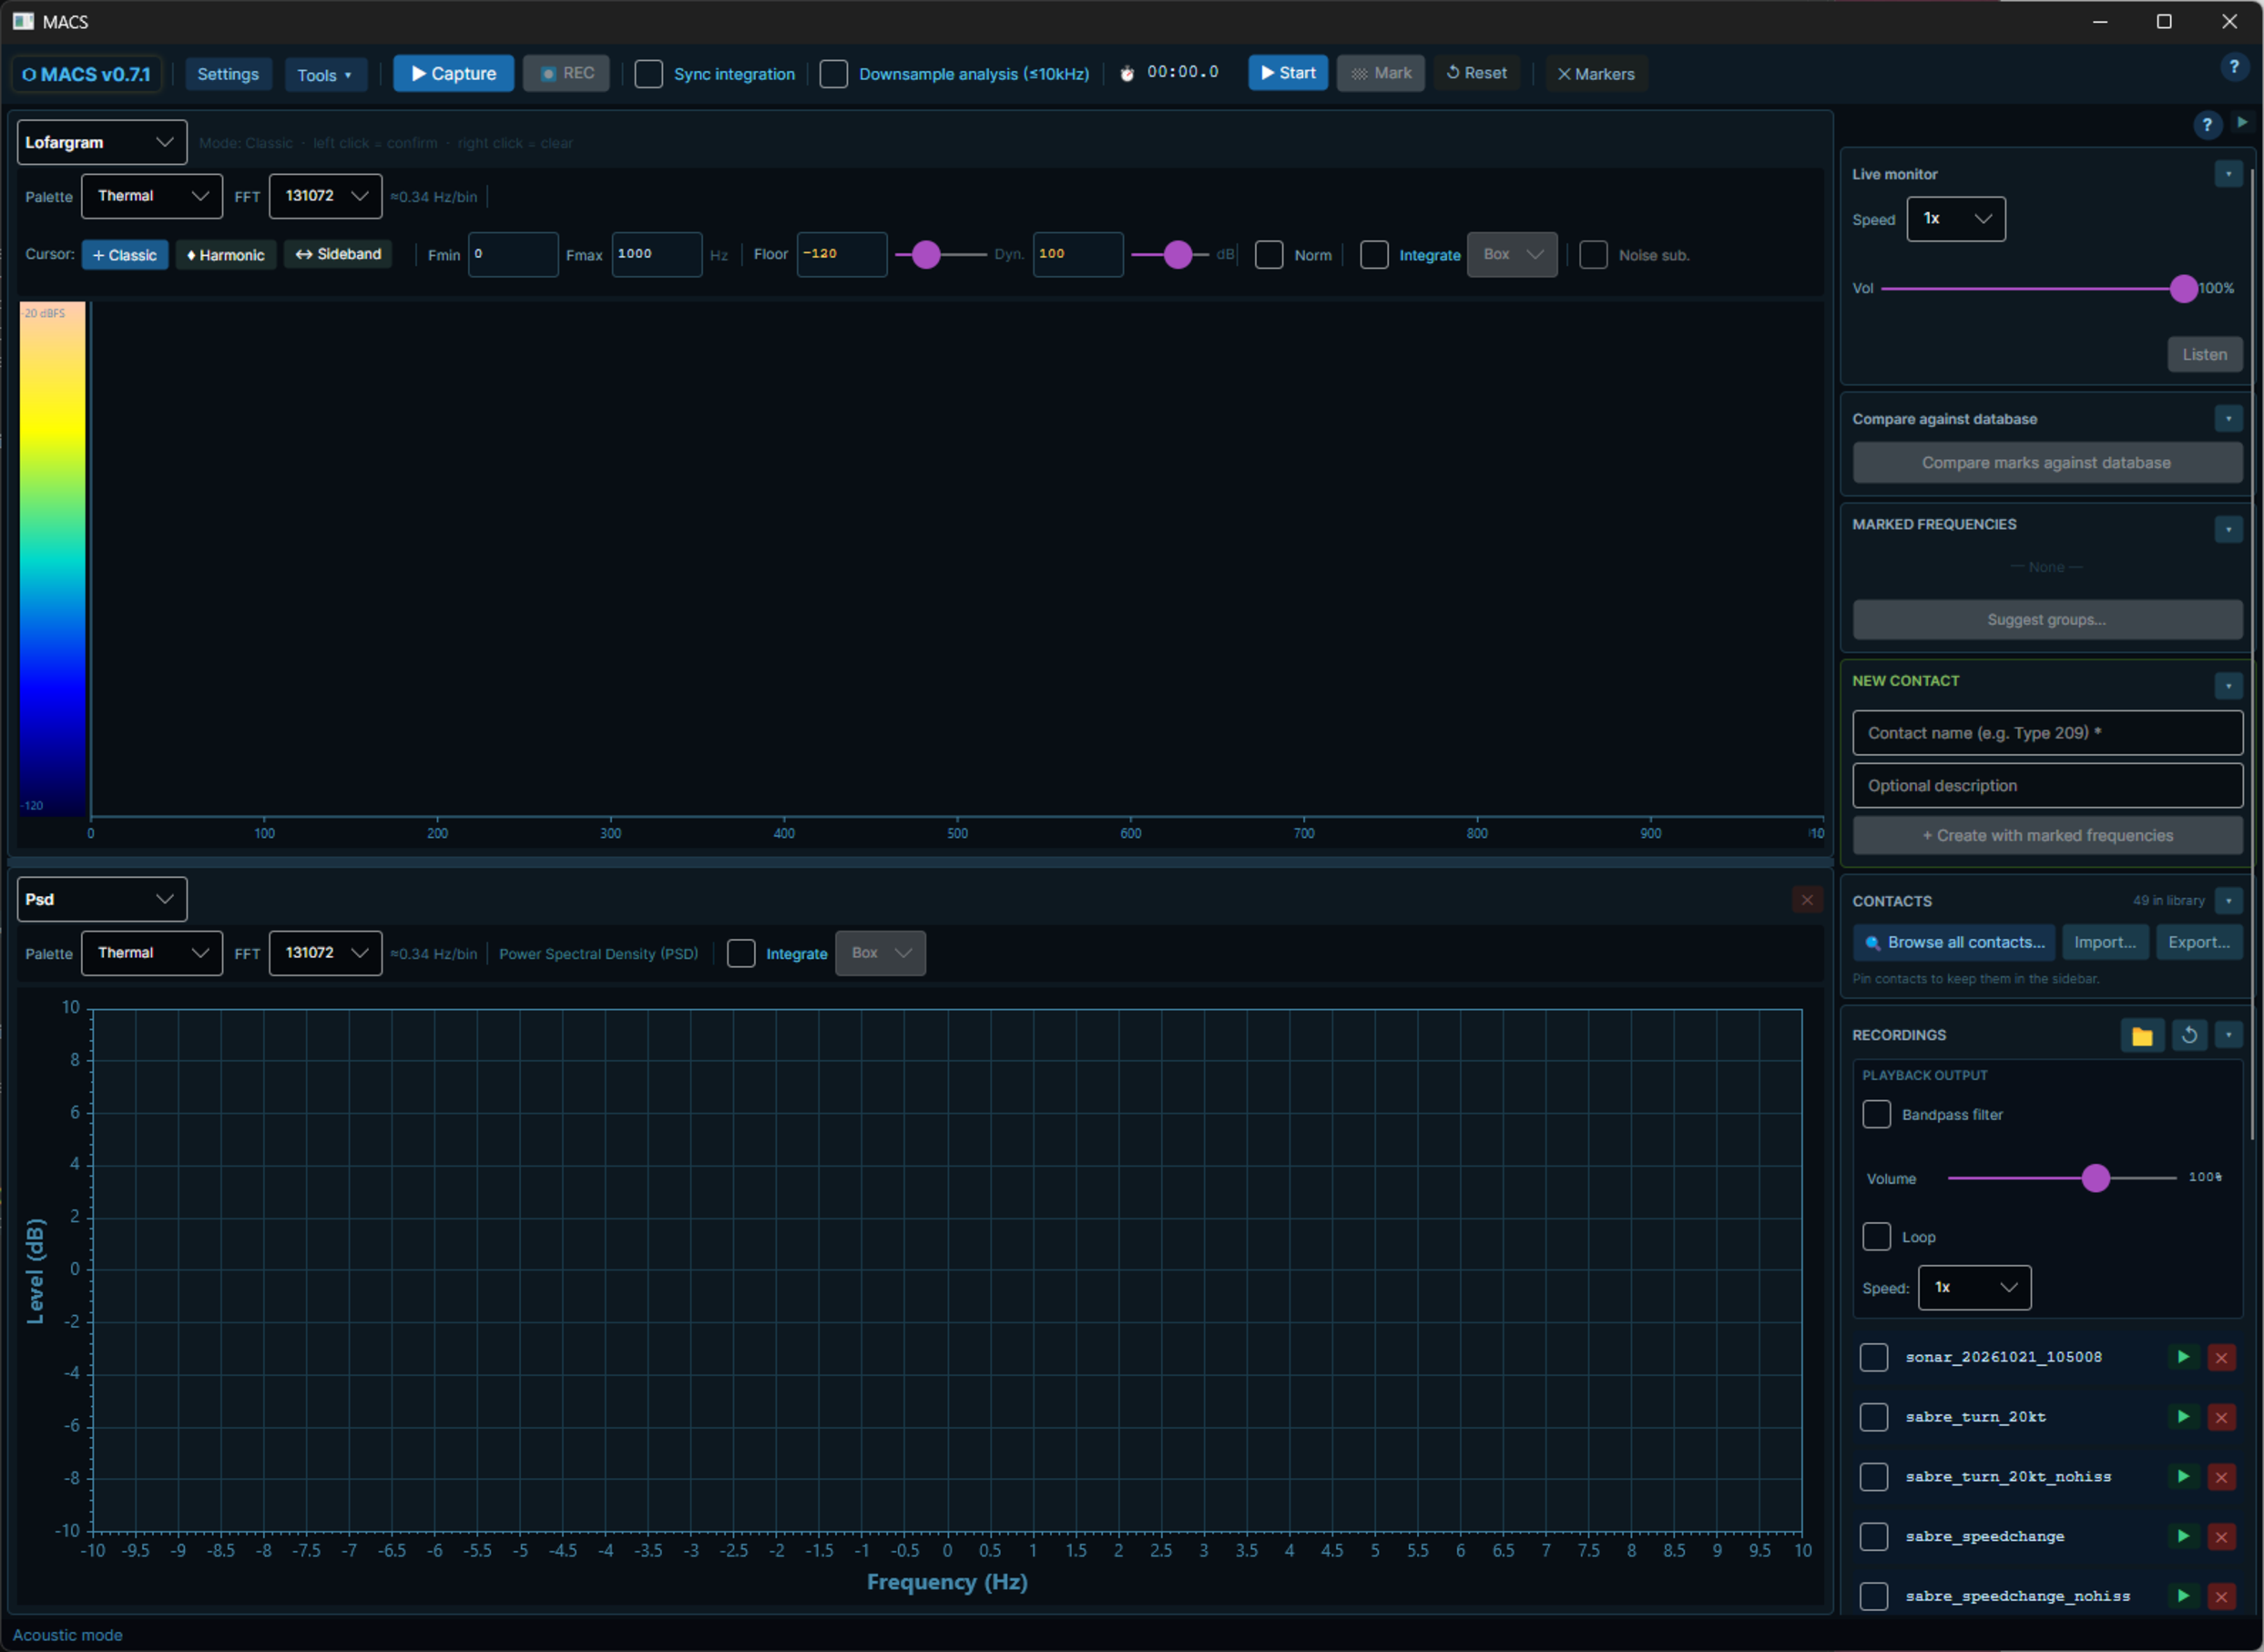
\includegraphics[width=345px]{../img/actuals/MACS.pdf}
	\caption{MACS Application Interface}
\end{figure}

\subsection{The Title Bar}

The title bar (Figure 2) has options to control the audio source, to start audio capture, manipulate the behaviours of Panel A and B, limit sample analysis and to enable recording for off line analysis. The title bar contains the following global controls:

\begin{figure}[h]
	\centering
	
\includegraphics[width=450px]{../img/actuals/topbar.pdf}
	\caption{The Title Bar}
\end{figure}

\begin{compactitem}
    \item \textbf{MACS Version:} Application version.
    \item \textbf{Settings:} View the settings panel.
    \item \textbf{Tools:} Dropdown to select tools.
    \item \textbf{Capture:} Starts live audio capture from the system (microphone / loopback).
    \item \textbf{REC:} Records the current capture to a WAV file in the recordings folder.
    \item \textbf{Sync Integration:} Synchronises settings between Panel A and B.
    \item \textbf{Downsample Analysis ($\le$ 10kHz):} Limits FFT / DEMON / Cepstrum / ACF to content $\le$ 10kHz.
    \item \textbf{Timer:} A useful timer with Start/Stop/Mark/Reset functionality.
    \item \textbf{Markers:} Toggles setting and deleting active frequency marker.
    \item \textbf{?:} On-screen guide to basic functionality, hover over options for on-screen guides.
\end{compactitem}

Hovering the mouse pointer over any of the controls will pop up an information box with more detail about it.
\pagebreak
\subsection{Main Panel - Central Analysis Area}

The main panel (Figures 3 and 4) hosts two display panels A and B. Both panels display a user select-able visual representations of the sound analysis performed by the application. Each panel has its own toolbar strip immediately above it, containing

\begin{compactitem}
    \item Content dropdown
    \item Palette selector
    \item FFT size
    \item Integrate
\end{compactitem}

In addition panel A has the following:

\begin{compactitem}
    \item Full cursor and display parameter row (Fmin / Fmax, Floor, Dynamic Range, Noise subtraction)
    \item Normalisation
\end{compactitem}

Panel B can be collapsed using its hide button. This does not stop its digital signal processing (DSP) pipeline it only removes the display from view. Showing it again immediately restores the waterfall.

Each panel has a dropdown at the top-left selecting its content type:

\begin{compactitem}
    \item LOFARgram Frequency-time waterfall (acoustic spectrogram)
    \item DEMON Envelope modulation waterfall (shaft rate detection)
    \item Cepstrum Quefrency-domain (see Appendix B) view for periodic structure
    \item ACF Running autocorrelation function
    \item PSD Live Power Spectral Density display (FFT size, sample rate, resolution, etc.)
\end{compactitem}

\begin{figure}[h]
	\centering
	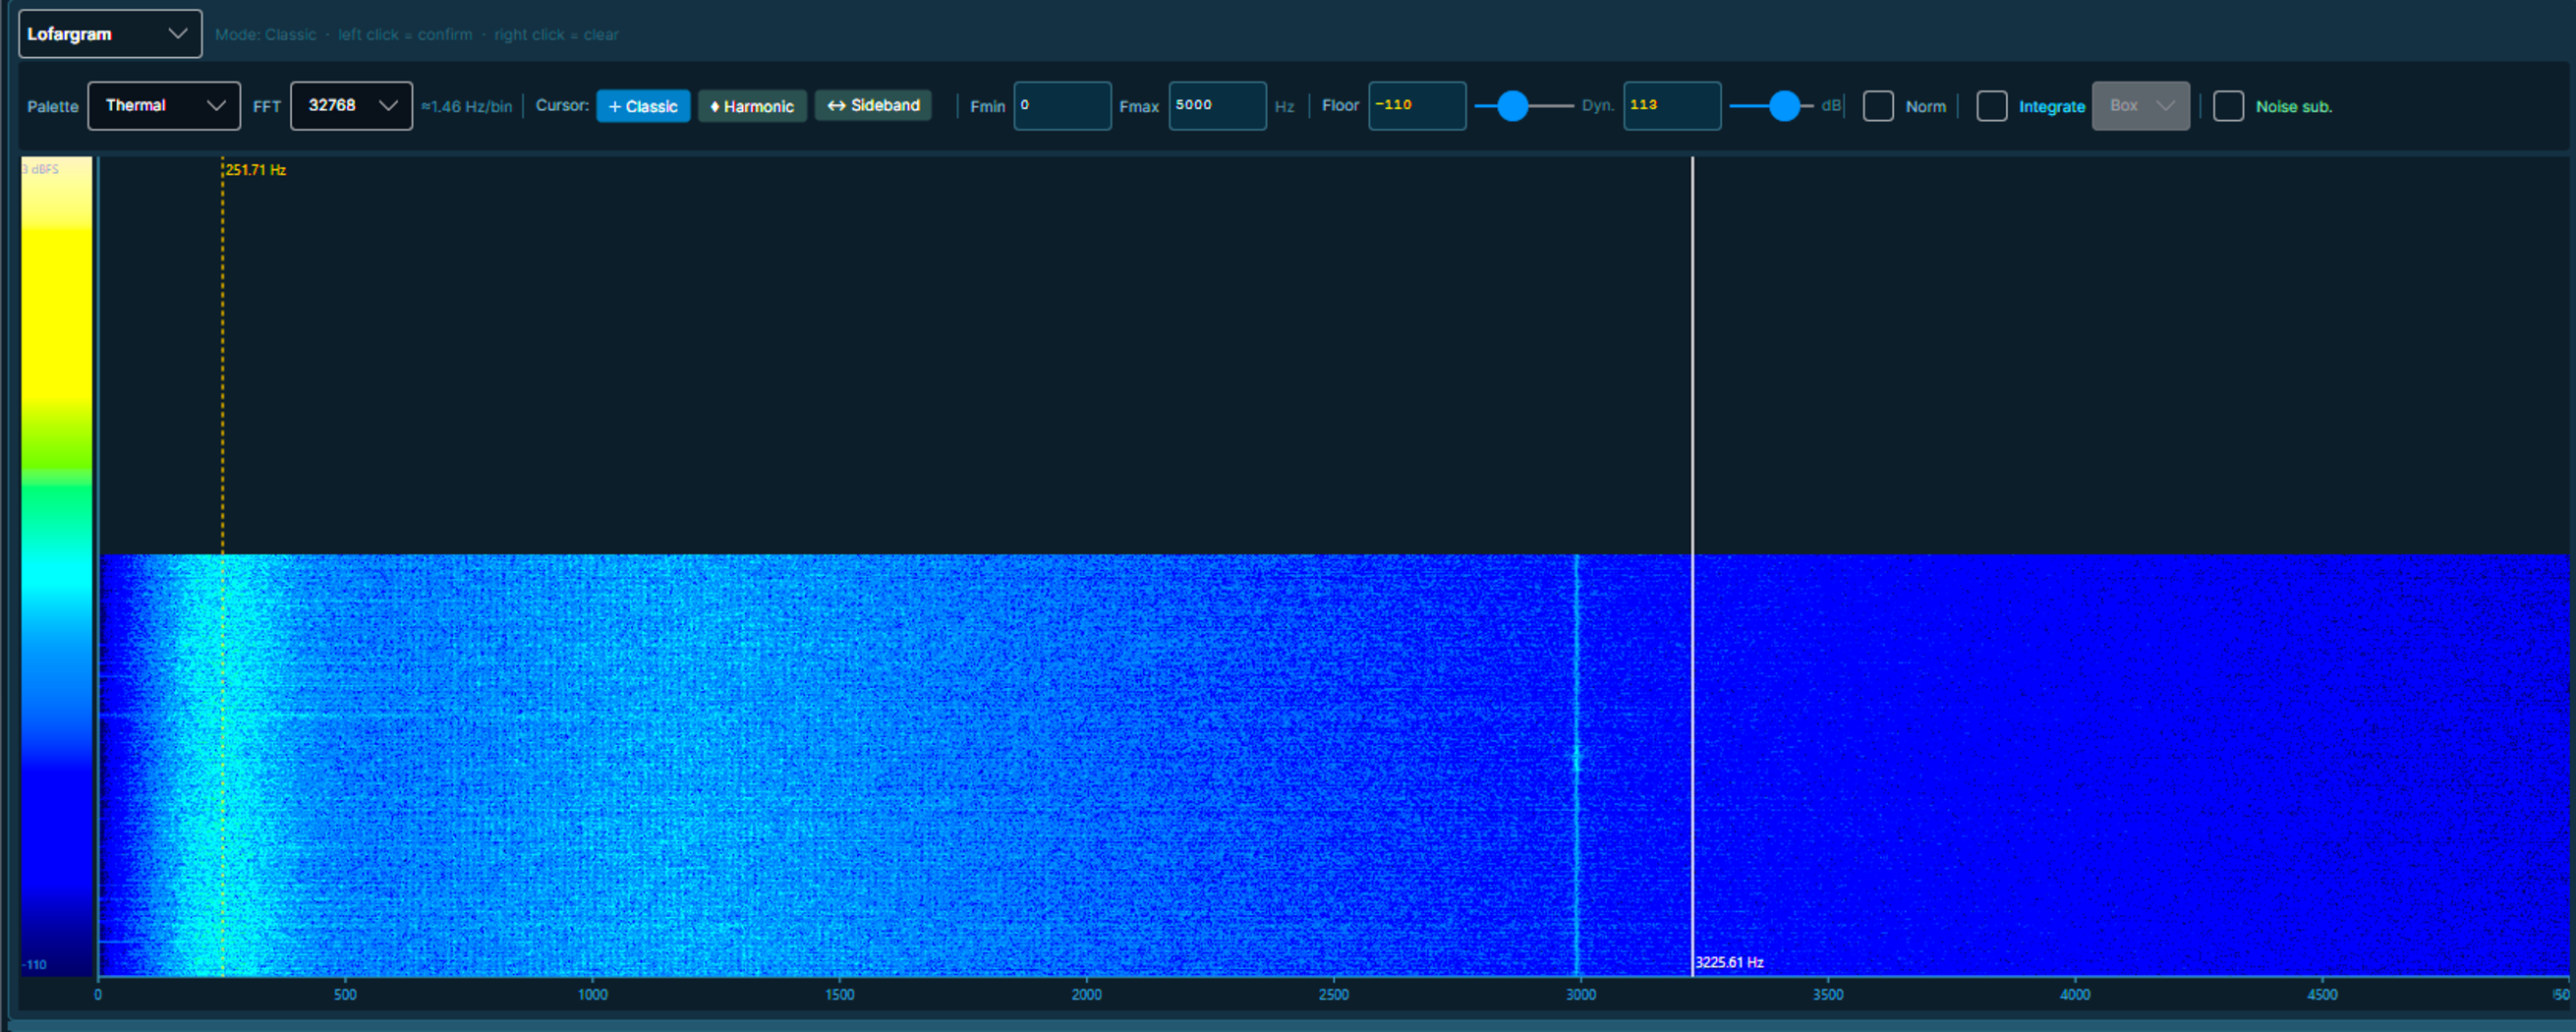
\includegraphics[width=400px]{../img/actuals/panel_A.pdf}
	\caption{Sub-panel A showing a LOFARgram}
\end{figure}

\begin{figure}[h]
	\centering
	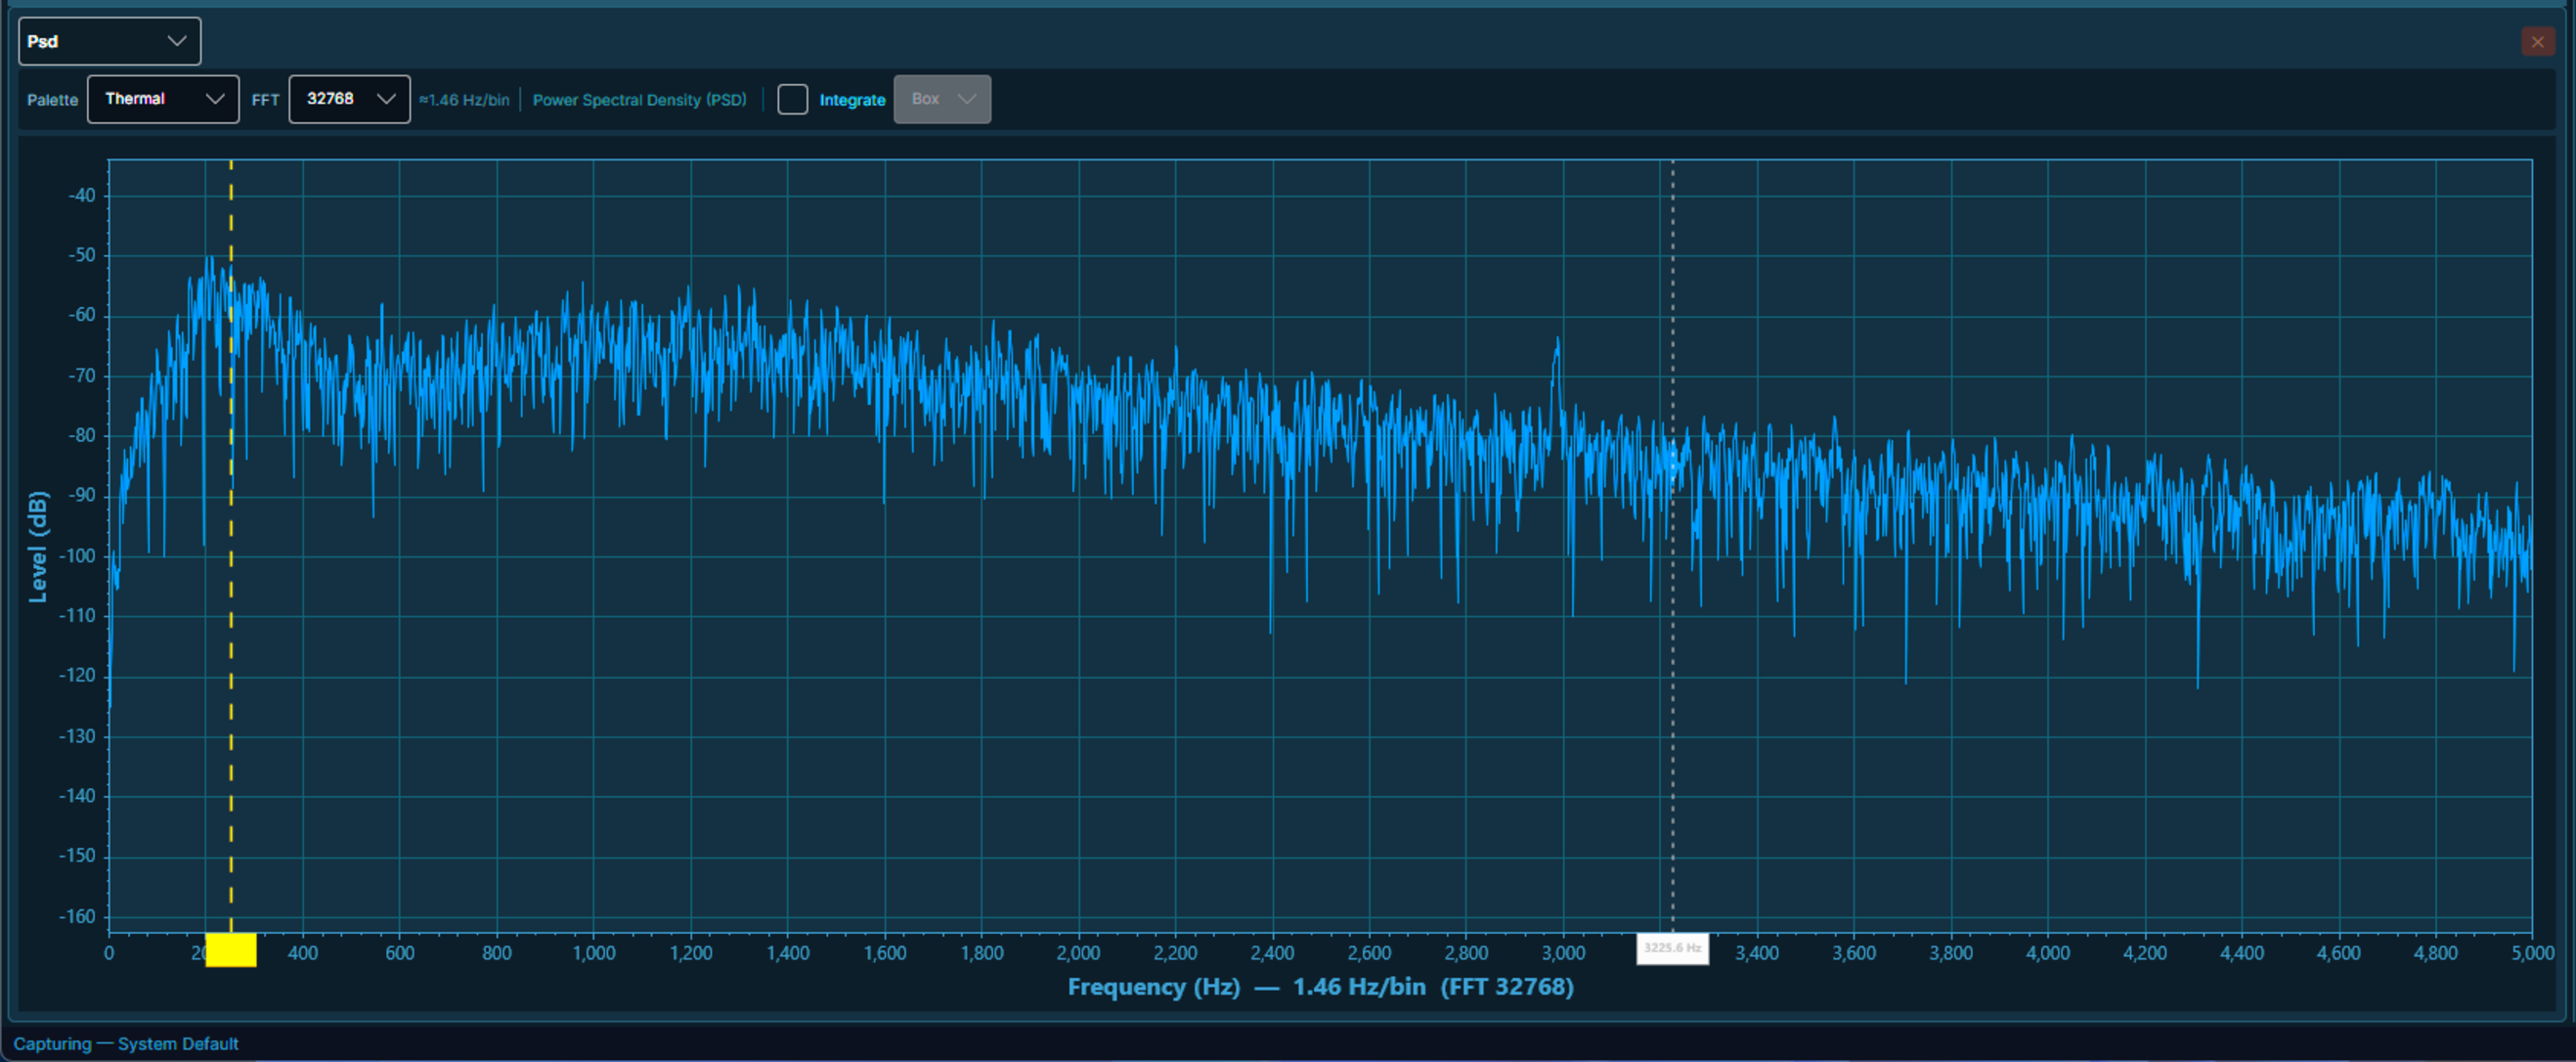
\includegraphics[width=400px]{../img/actuals/panel_B.pdf} % \textwidth
	\caption{Sub-panel B showing the Psd display}
\end{figure}

Each display type has a toolbar with controls specific to its content type. These appear above the panel's display area.

\subsubsection{LOFARgram / DEMON toolbar}
\textcolor{commentGreen}{*** WIP ***}

\textbf{LOFARgram:}

\begin{compactitem}
    \item Palette: Colour palette for the waterfall display. The default is a perceptually uniform palette (Viridis) which is good for visualising low SNR signals.
    \item FFT Size: Number of FFT points (before zero-padding). Larger = better frequency resolution, slower time resolution. Powers of 2: 4096 $\rightarrow$  131072 with $\approx$ 0.34 Hz Bins.
    \item Cursor: Classic, Harmonic and Sideband modes. Shows the current cursor position in time / order and frequency.  Classic shows the cursor position in time and frequency. Harmonic mode shows the cursor position in time and shaft rate (Hz) and displays the harmonic series of the current cursor position. Sideband shows the sidebands either side of the target tonal with their separation in Hz. The cursor can be moved by clicking on the waterfall or by dragging the cursor marker.
    \item $F_{min}$ / $F_{max}$: Display frequency limits (Hz). Crops the visible axis without affecting the pipeline.
    \item Floor (dB): The amplitude level that maps to the coldest colour. Signals below this are clipped to black.
    \item Dyn (dB): Dynamic range: the amplitude span from Floor to the hottest colour. Floor + Dyn = the level that maps to maximum brightness.
    \item Floor slider: Coarse adjustment for Floor.
    \item Dyn slider: Coarse adjustment for Dynamic Range.
    \item Normalisation: Adjusts the waterfall display to compensate for the frequency response of the capture device. See Appendix B for more information.
    \item Integrate: Integration across the live frames improves Signal to Noise Ratio (SNR). Best used for loitering or slow moving targets as moving targets will smear rather than sharpen.
    \item Noise Subtraction: Subtracts a reference noise profile from the waterfall. \textcolor{commentGreen}{*** WIP ***}
\end{compactitem}

\textbf{DEMON:}

\begin{compactitem}
    \item Palette: As for LOFARgram
    \item FFT Size: As for LOFAR but restricted range 256 $\rightarrow$ 4096 with $\approx$ 0.12 Hz Bins.
    \item Cursor: Classic and Harmonic cursor modes. Classic shows the cursor position in time and frequency. Harmonic mode shows the cursor position in time / order and shaft rate (Hz) and displays the harmonic series of the current cursor position.
    \item RPM: Show the cursor frequency in RPM
    \item Blades: \textcolor{commentGreen}{*** WIP ***}
    \item Band: The acoustic frequency band fed into the DEMON envelope detector. Narrowing this to a band with strong broadband noise (e.g. 500 - 5000 Hz) improves signal to noise ratio (SNR).
    \item $F_{max}$: Display frequency limits (Hz). Crops the visible axis without affecting the pipeline.
    \item Floor (dB): The amplitude level that maps to the coldest colour. Signals below this are clipped to black.
    \item Dyn (dB): Dynamic range: the amplitude span from Floor to the hottest colour. Floor + Dyn = the level that maps to maximum brightness.
    \item Floor slider: Coarse adjustment for Floor.
    \item Dyn slider: Coarse adjustment for Dynamic Range.
\end{compactitem}

\subsubsection{Cepstrum / ACF toolbar}
\textcolor{commentGreen}{*** WIP ***}

Same controls as above; Fmin / Fmax instead control the quefrency display range in ms.

\subsubsection{Power Spectral Density (PSD)}
\textcolor{commentGreen}{*** WIP ***}
Power Spectral Density (PSD) analysis is a signal-processing technique used to show how the power (or energy) of a signal is distributed across frequency.

In simple terms:
\begin{compactitem}
    \item A time-domain signal shows how a measurement changes with time.
    \item A PSD shows which frequencies contain the most power.
\end{compactitem}

This makes PSD one of the most useful tools for analysing sounds, vibrations, machinery, sonar recordings, and electrical signals.

\subsubsection{ZoomFft}
\textcolor{commentGreen}{*** WIP ***}

ZoomFFT is particularly useful for:
\begin{compactitem}
    \item Resolving closely spaced shaft-rate harmonics
    \item Measuring small frequency shifts due to vessel speed changes
    \item Separating propeller blade-rate sidebands
    \item Examining a narrow cavitation band with much higher resolution than a full-band FFT
\end{compactitem}

\begin{tabularx}{\linewidth}{l X X}
    \toprule
    \textbf{Feature} & \textbf{FFT} & \textbf{ZoomFFT}\\
    \midrule
    Frequency Range & Entire spectrum & Narrow selected band \\
    Computational cost & Higher for fine resolution & Lower \\
    Resolution in region of interest & Requires very long FFT & Very High\\
    Real-time operation & More demanding & Efficient \\
    Requires frequency translation & No & Yes \\
    \bottomrule
\end{tabularx}

Imagine looking at a ship on the horizon. A normal FFT is like viewing the whole sea with your naked eye but a ZoomFFT is like pointing a telescope at just the ship. You do not gain extra information about the rest of the sea, but you see much finer detail where you're looking. For LOFAR analysis, ZoomFFT is often the preferred way to examine a narrow harmonic family (for example around a shaft rate harmonic or blade-pass frequency) without needing an enormous FFT length.

If you are analysing a signal and already have reason to believe that a narrowband component of interest lies near 42 Hz, you could centre a ZoomFFT at 42 Hz to examine that region at finer frequency resolution.

\begin{compactitem}
    \item Harmonic splitting,
    \item Modulation sidebands,
    \item Slight RPM fluctuations,
    \item Blade-pass sidebands.
\end{compactitem}

This often produces much cleaner results than performing an enormous FFT over the entire acoustic band. For machinery diagnostics and marine acoustics, ZoomFFT is essentially a software implementation of a narrowband spectrum analyser.

\subsection{Settings Panel}

\begin{figure}[ht]
	\centering
	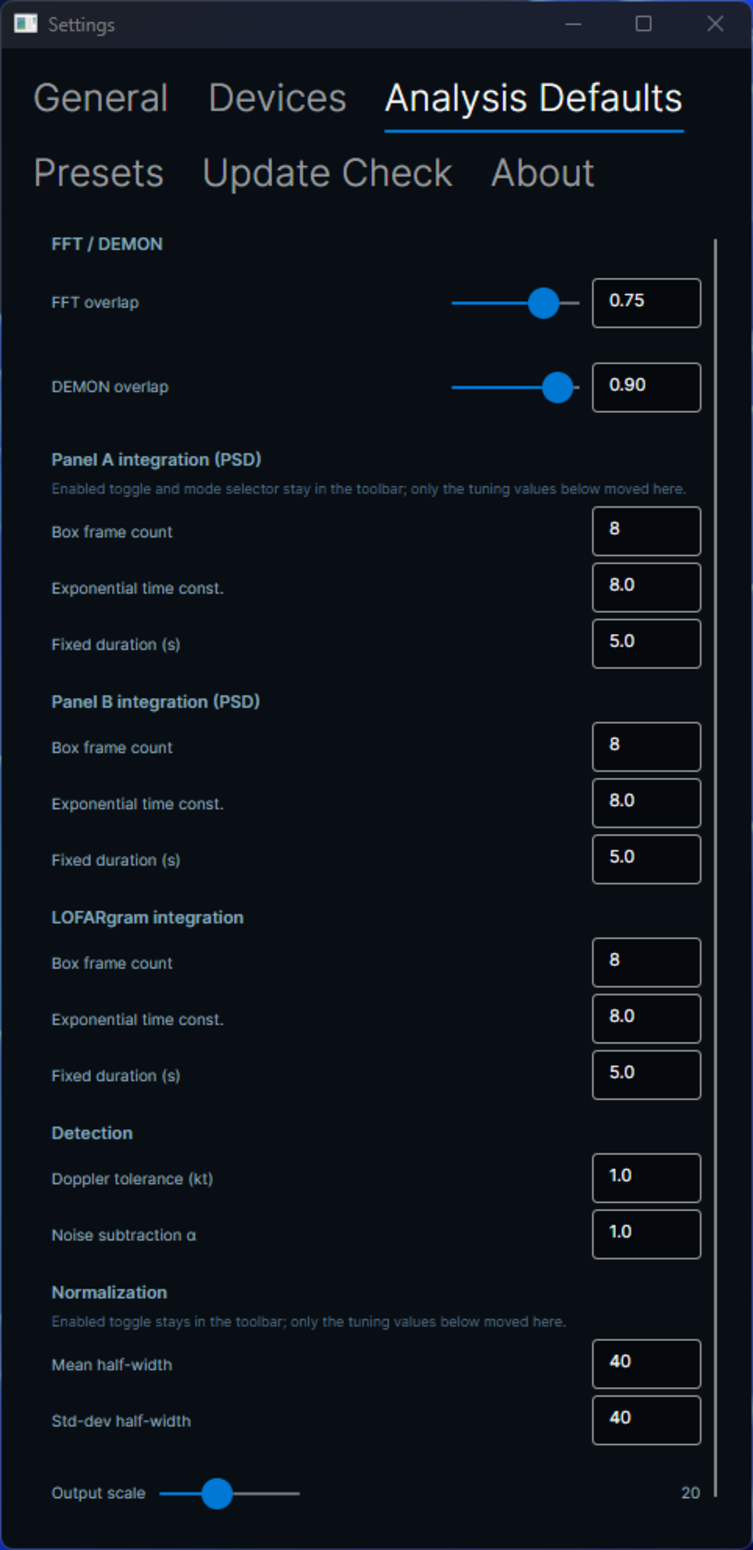
\includegraphics[width=150px]{../img/actuals/analysis.pdf}
	\caption{Analysis Defaults panel}
\end{figure}

Clicking the settings button in the title bar opens a panel with the following control subpages:

\begin{compactitem}
    \item \textbf{General} Allows setting the location of the user recordings folder, defaults to the user's Documents folder.
    \item \textbf{Devices} Sets the sound capture device, the live monitor output device and the recording playback device.
    \item \textbf{Analysis Defaults} Sets FFT / DEMON overlap, panels A/B overlap and integration features (see Figure 5).
    \item \textbf{Presets }Allows user to set up to 5 presets for the analysis parameters (FFT size, overlap, Fmin / Fmax, Floor, Dynamic range, DEMON parameters). Presets are saved to the settings file and restored on next launch.
    \item \textbf{Update Check} Checks for a new version of the application and prompts the user to download it if available.
    \item \textbf{About} View the application version and license information.
\end{compactitem}

\subsection{Right sidebar - Contact Recording and Management}

The right sidebar has two main functions. Capturing and managing contact's sound profiles and matching an unknown sound profile with previously captured ones. It is also used to set up a background sound file which can be used for noise subtraction. Because the use of the contact database and the recording feature is an important part of MACS it has its own section (Section 4).

The right sidebar has a third function, the live monitor. This is a simple audio output of the current capture device. It is useful for checking that the capture device is working and for listening to the sound being captured. The live monitor can be muted or set to a different output device than the capture device.
\pagebreak
\subsection{Noise Subtraction}

In a noisy environment it is often difficult to distinguish potential target tonals from the background. This is often the case in shallow waters. MACS Noise Subtraction allows the user to diminish the effect of this environmental noise. This is achieved by utilizing a pre-recorded sound file of the local environment and then mathematically subtracting it from the live sound. Obviously, this requires that you make a recording of the environment which only has ambient background noise. The mathematical process used is described in detail in Appendix B.

The following steps the user through the process

\begin{compactenum}
    \item Make a recording of the ambient environmental noise and store that for later use. The file must be at least \textbf{15 seconds long} (enforced by validation). Short files produce unstable spectral averages.
    \item When the time comes to use the file select the WAV file that contains \textbf{only ambient/background noise} --- no contact of interest.
    \item Check the \textbf{\enquote{Use as noise reference}} checkbox next to that recording. Only one reference can be active at a time (exclusive selection --- checking one unchecks any previous reference).
    \item Click \textbf{\enquote{Noise sub}} checkbox on the LOFAR panel toolbar to compute and store the reference spectrum.
\end{compactenum}

MACS then attempts to reduce the effect of environment noise which you should observe as the time window progresses.

\begin{advisory}
    \textbf{Note: }The result of noise subtraction can vary due to many confounding factors however it is worth trying if the environment you are operating is particularly noisy. Also noise subtraction will not be effective against some natural sound which have an unpredictable pattern, e.g. whale sounds. More stable natural frequencies such as shrimp may be reduced. That magmatic anomaly will still stand out though. Also noise subtraction may have the unintended effect of hiding the very tonals you are looking for.
\end{advisory}

\subsection{The Cursor System}

The cursor system allows the user to mark individual tonals, identify harmonics and assess sidebands. Select a cursor mode from the toolbar before clicking on the waterfall then click on the tonal you wish to mark.

\begin{compactitem}
\item \textbf{Single:} Places one frequency marker at the clicked frequency $f$.
\item \textbf{Harmonic:} Places harmonic series line starting from the fundamental + N harmonics above it. Configurable N and line width.
\item \textbf{Sideband} Adds sideband lines on both sides of $f$ using the specified spacing $\Delta$ and line count N. "Right only" shows only lines to the right of $f$ (upper sideband).
\end{compactitem}

\subsection{Settings Persistence}

In Windows parameters are saved automatically to \path{C:\Users\%user%\AppData\Roaming\MACS\settings.json}. On Linux and macOS the settings file is located in \path{~/.config/MACS/settings.json}.

This includes: FFT size, overlap, Floor, Dynamic range, Fmin / Fmax, normalisation parameters, DEMON parameters, noise reference path, filter settings, and recordings folder path.

Settings are restored on next launch. If you need to reset to defaults, delete \path{C:\Users\%user%\AppData\Roaming\MACS\settings.json} or \path{~/.config/MACS/settings.json} and restart the application.
\pagebreak
\section{Contact Database and User Recordings}
\subsection{Overview}
The contact database stores known acoustic signatures allowing you to build a library of known contacts, and to compare current contacts with those in the database. The database is stored in a single file called \path{sonar.db} in the MACS application data folder. The database is created automatically when MACS is first run, and is empty until you add your own contacts. Further details about the fields and structure of the database are discussed in Appendix C. MACS also allows you to record contacts and store them in the database. The recordings are stored in a separate folder, which is set in the \textbf{Settings} panel.

\begin{faintquote}
    This section provides a basic outline of the process and workflow for contact recording and matching. A more detailed process workflow is given in the Illustrated Examples section.
\end{faintquote}

\subsubsection{Installing the pre-populated database}
If you wish you can install a pre-populated database of known contacts. At the time of writing this database contains all of the vessels included in the MNW Recognition Guide, excluding aircraft, and is intended to be a starting point for your own database. As such it does not contain the LOFARgram details. It is assumed that users would prefer to update the database with their own recordings. To install the database:

\begin{compactenum}
    \item Download the \href{https://github.com/Mahzel/MACS}{MNW Defaults} database file from the MACS website.
    \item \verb|MNW_Defaults.db| will download to users Download folder
    \item Open MACS
    \item In the right panel select Import from the Contacts subpanel
    \item Follow on screen direction to install the prepopulated database
\end{compactenum}

\subsection{Contact Database}
\subsubsection{Terminology}
\begin{compactitem}
    \item Contact: A hull with defined constants e.g. name, propulsion type, nationality etc.
    \item Measurement: An observation made with the tools, attached to a contact. A single contact can have multiple measurements.
    \item Recording: A sound file containing a contact's acoustic signature. %Recordings are linked
\end{compactitem}

\subsubsection{Database Interface}
The database and recordings management panels are on the right side of the application window Figure 6. The right side panels can be hidden by clicking the right pointing arrow and the sub-panels can be collapsed to save space. The database panel has the following sub-panels:

\begin{compactitem}
    \item Compare against database: Shows a list of all contacts in the database which match your marked frequencies.
    \item Marked frequencies:
    \item New contact: Allows you to add a new contact to the database.
    \item Contacts: Browse, import and export contacts.
\end{compactitem}

The recordings panel shows a list of all recordings in the recordings folder, and allows you to add, rename and delete recordings.

To add a recording to the database first make sure that the in-game sound is being captured by MACS. Then click the \enquote{\textbf{REC}} button on the applications Top Tool Bar. You should capture a recording of sufficient length to ensure that you have captured a full range of sounds. On playback the recording can be looped so that it appears continuous when you are performing an analysis. The panel allows an adjustment of playback speed which is very useful when you are trying to count regular sounds like propeller blades. It also allows you to apply a bandpass filter to the playback, which is useful for listening to specific frequency ranges.

\begin{compactitem}
    \item To rename a recording, double click the name and enter a new name.
    \item To delete a recording, click the red cross.
\end{compactitem}

\begin{figure}[ht]
	\centering
	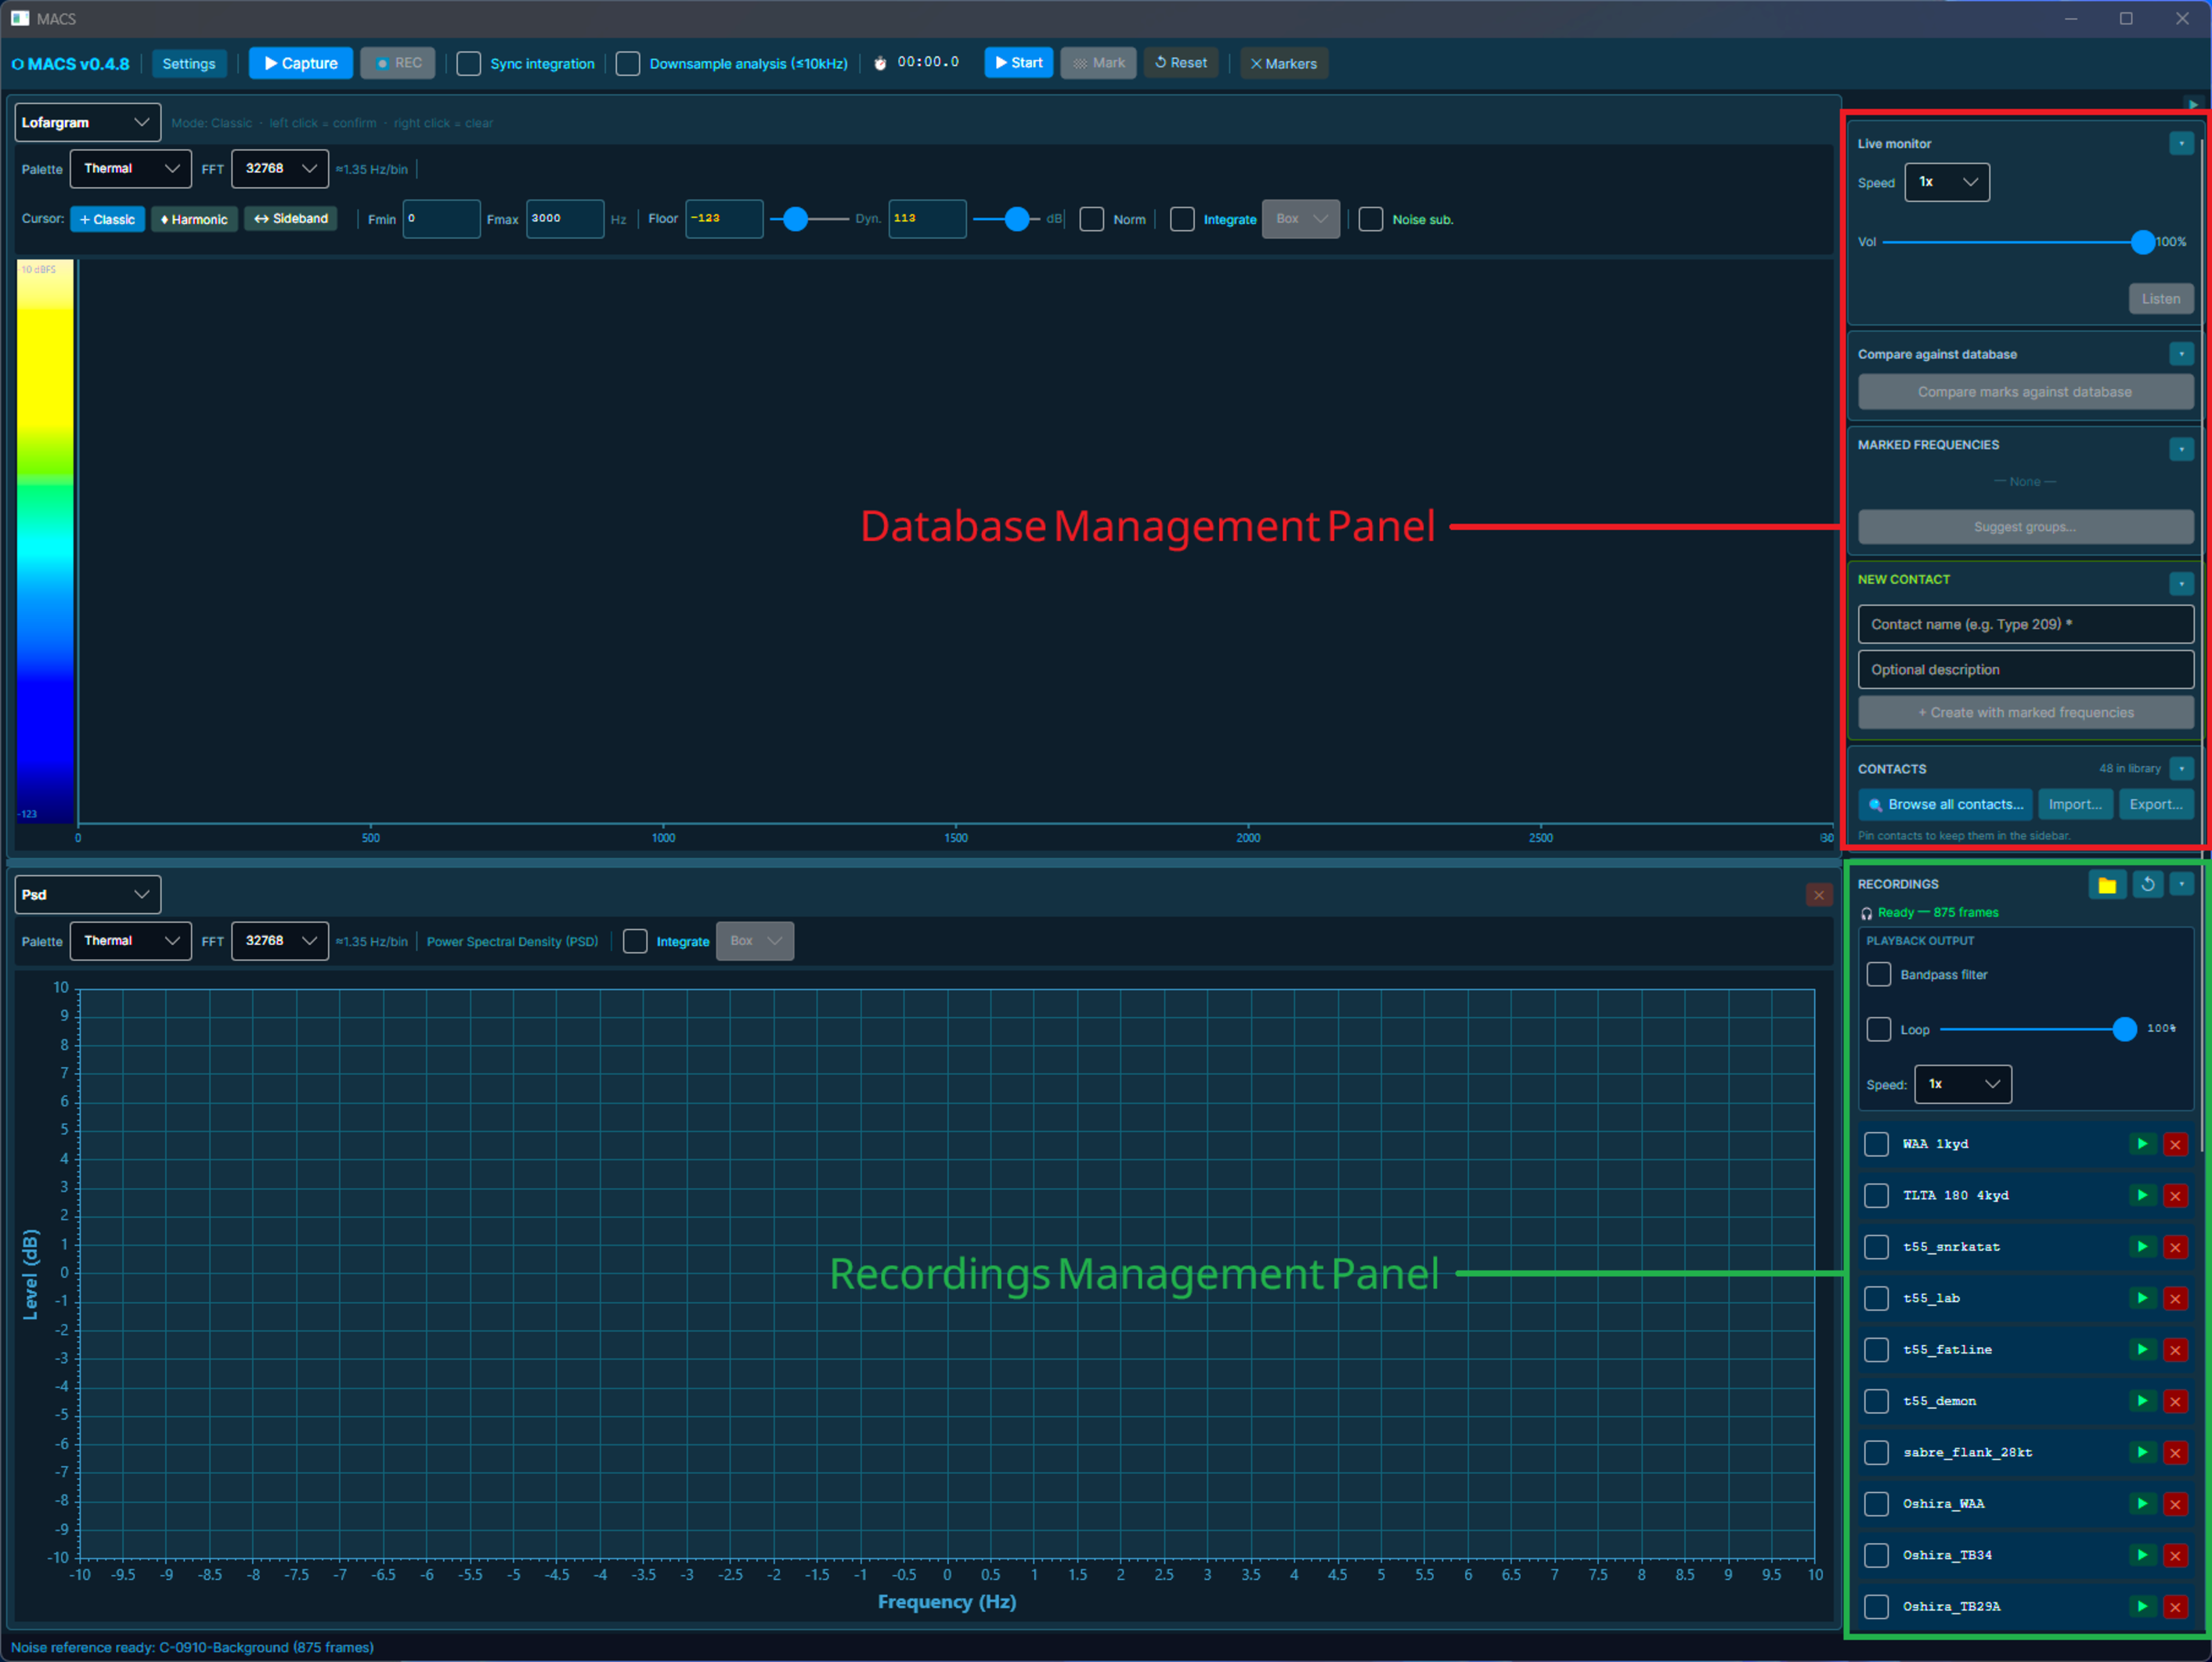
\includegraphics[width=400px]{../img/actuals/MACS_RecordingPanels.pdf}
	\caption{MACS Database and Recordings Panels}
\end{figure}

\subsection{Contact Management}
To browse the contacts in the database, click the \textbf{Browse all contacts} in the \textbf{Contacts} sub-panel Figure 7. This opens the \textbf{Contacts Library} window. Here you can filter the list by entering text in the search box, by tag or by confidence level. The library widow gives you access to the \textbf{Contact Information} panel Figure 8 by clicking either the folder icon or the data icon next to the units name. Both open the same window but at different tabs. The Contact Information window allows you to:

\begin{compactitem}
    \item Enter general information about the contact name, class, nationality, classification confidence etc.
    \item Enter propulsion details, engine type etc.
    \item Ability to set ownship (sets overlay colour to red if checked).
\end{compactitem}

\pagebreak

\begin{figure}[ht]
	\centering
	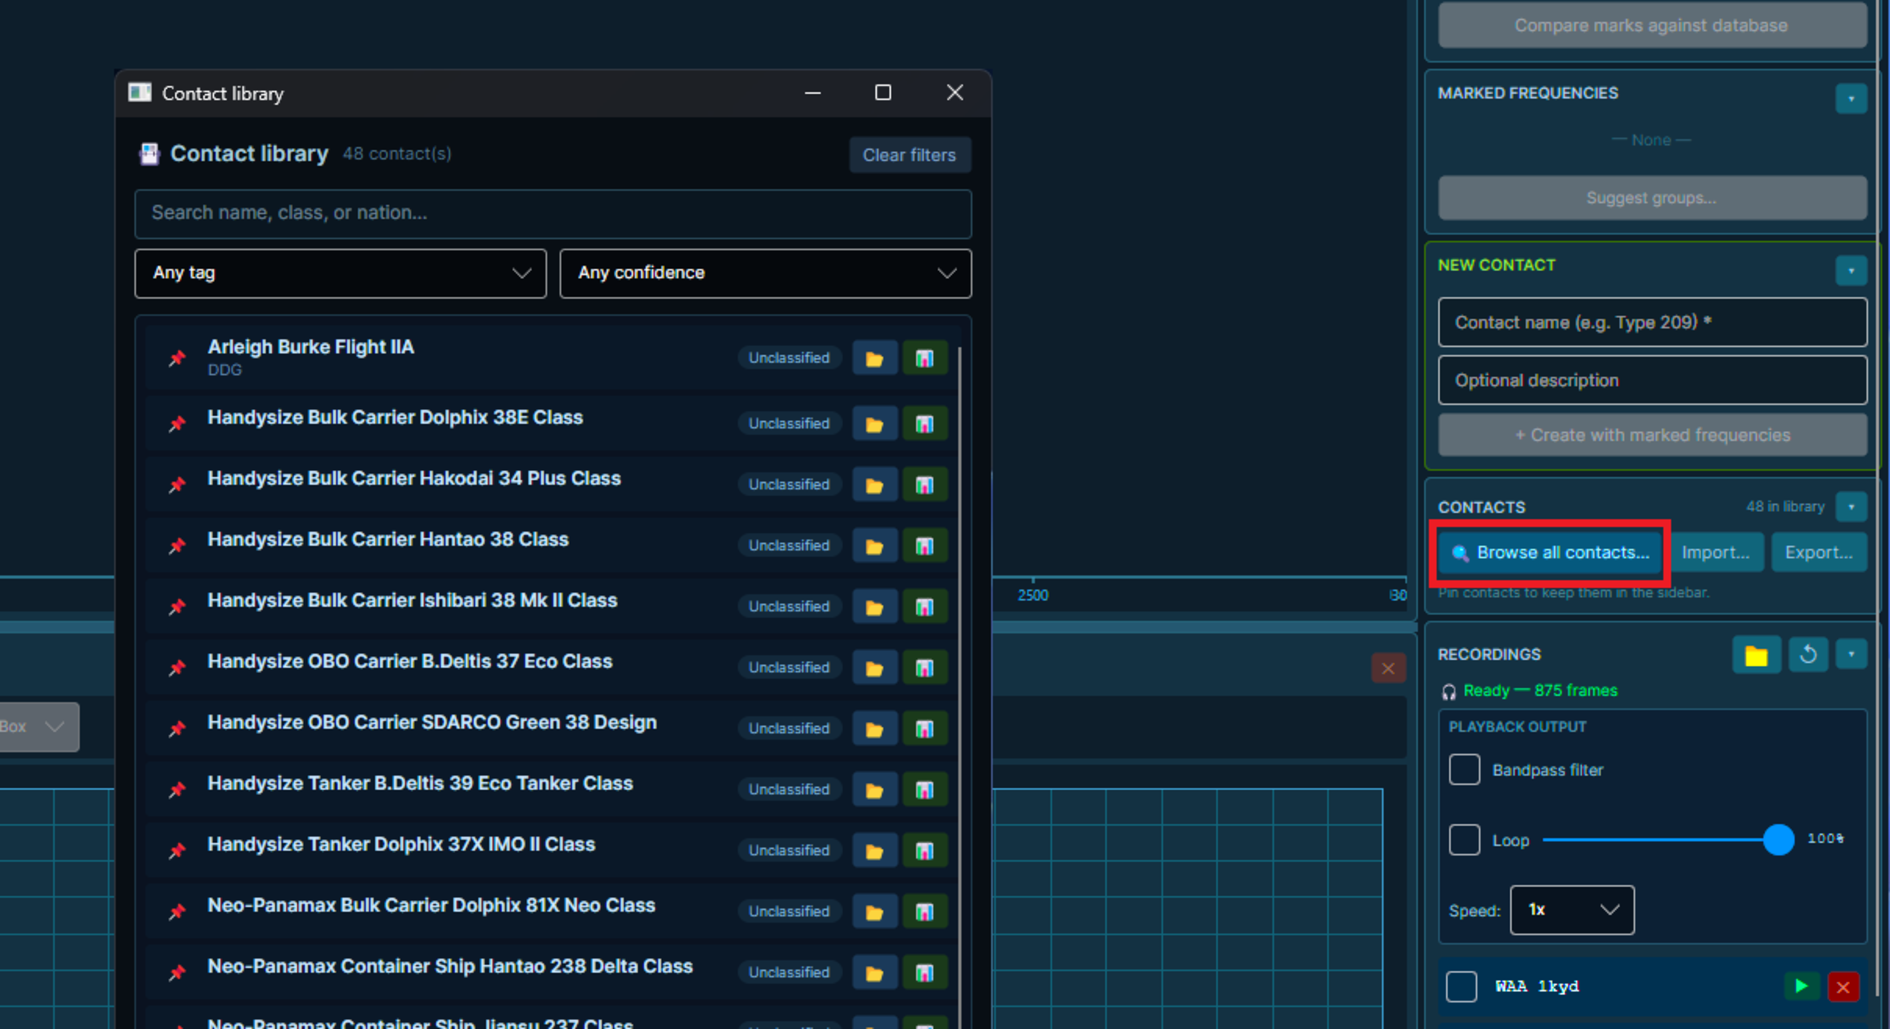
\includegraphics[width=400px]{../img/actuals/BrowseContacts.pdf}
	\caption{Contact Browsing}
\end{figure}

\begin{figure}[ht]
	\centering
	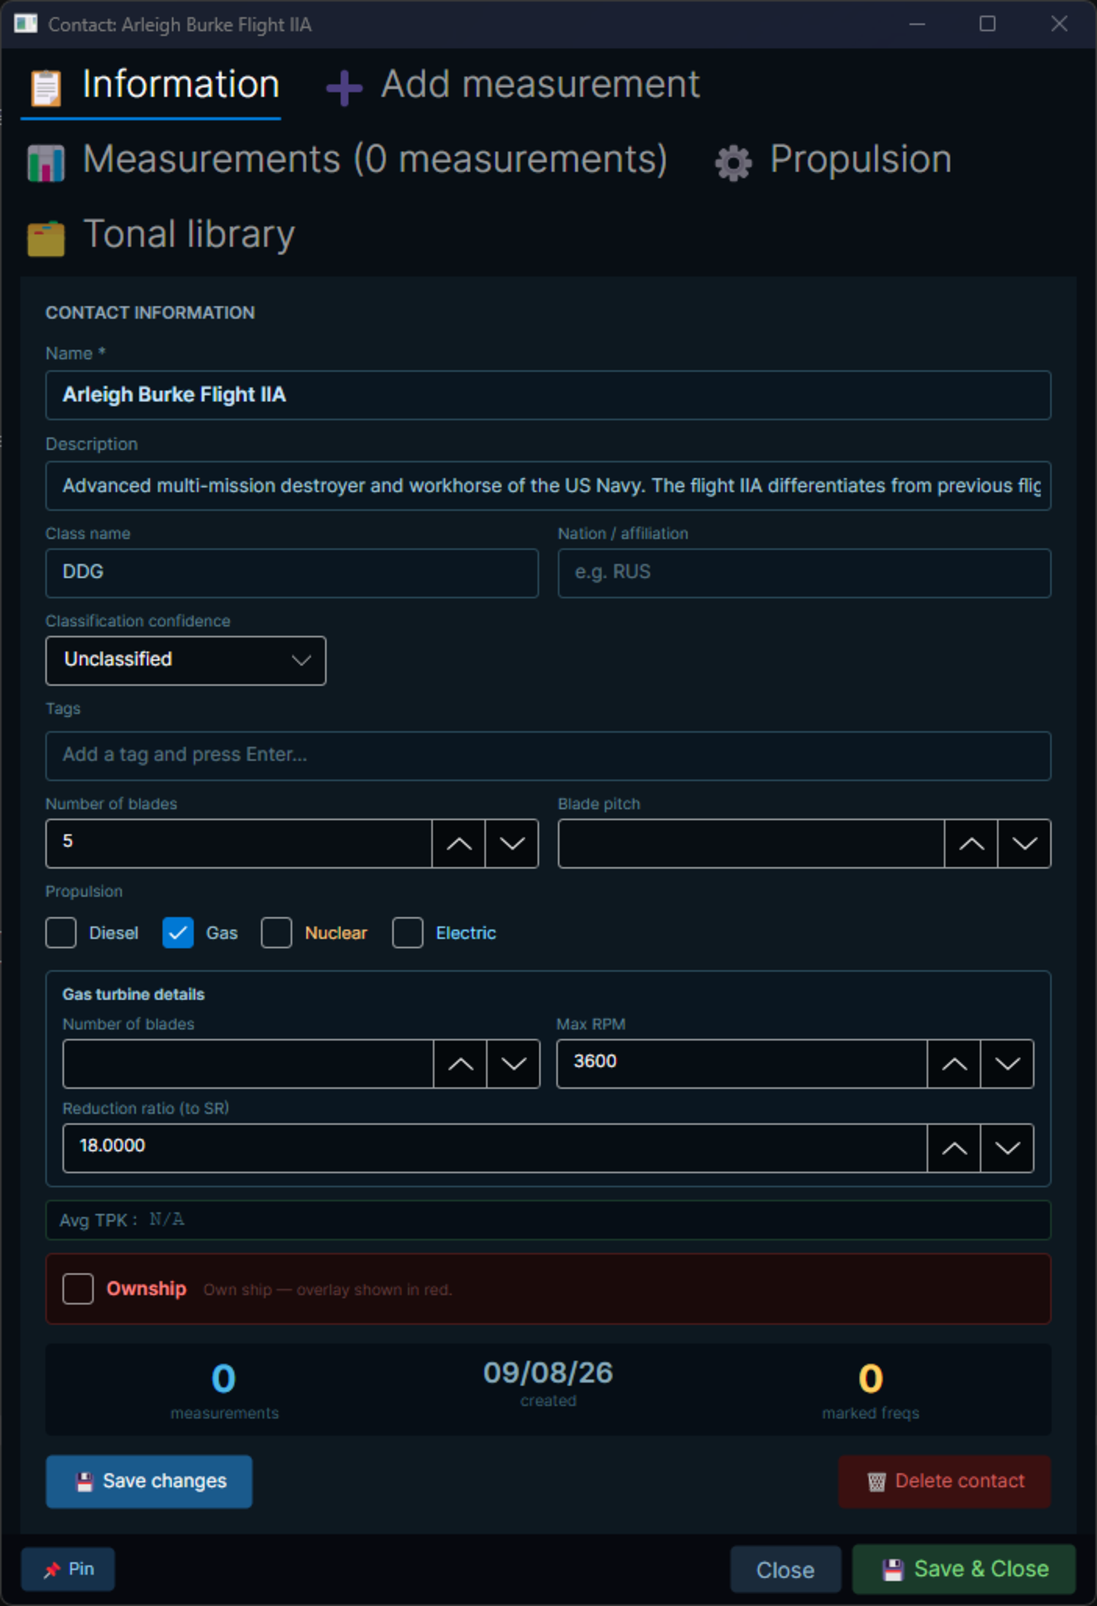
\includegraphics[width=175px]{../img/actuals/MeasurementsPanel.pdf}
	\caption{Measurements Panel}
\end{figure}

\begin{faintquote}
    Note: Saving changes or new measurements requires the user to click the \enquote{\textbf{Save Changes}} button on the left of the panel below the \enquote{\textbf{Ownship}} select box \textbf{before} clicking \enquote{\textbf{Save and Close}}. Just clicking save and close closes the panel without saving the changes.
\end{faintquote}

\subsection{Creating a New Contact}
\textcolor{commentGreen}{*** WIP ***}

To add a new contact at least one frequency must be marked on the LOFARgram (Figure 9). Prominent lines are obvious choices as are the shaft, blade and crankshaft rates. If possible identify the electrical mains and generator set tonals (50 hz or 60hz). These do not slide with speed changes in the same way that some other measures do.

\begin{figure}[ht]
	\centering
	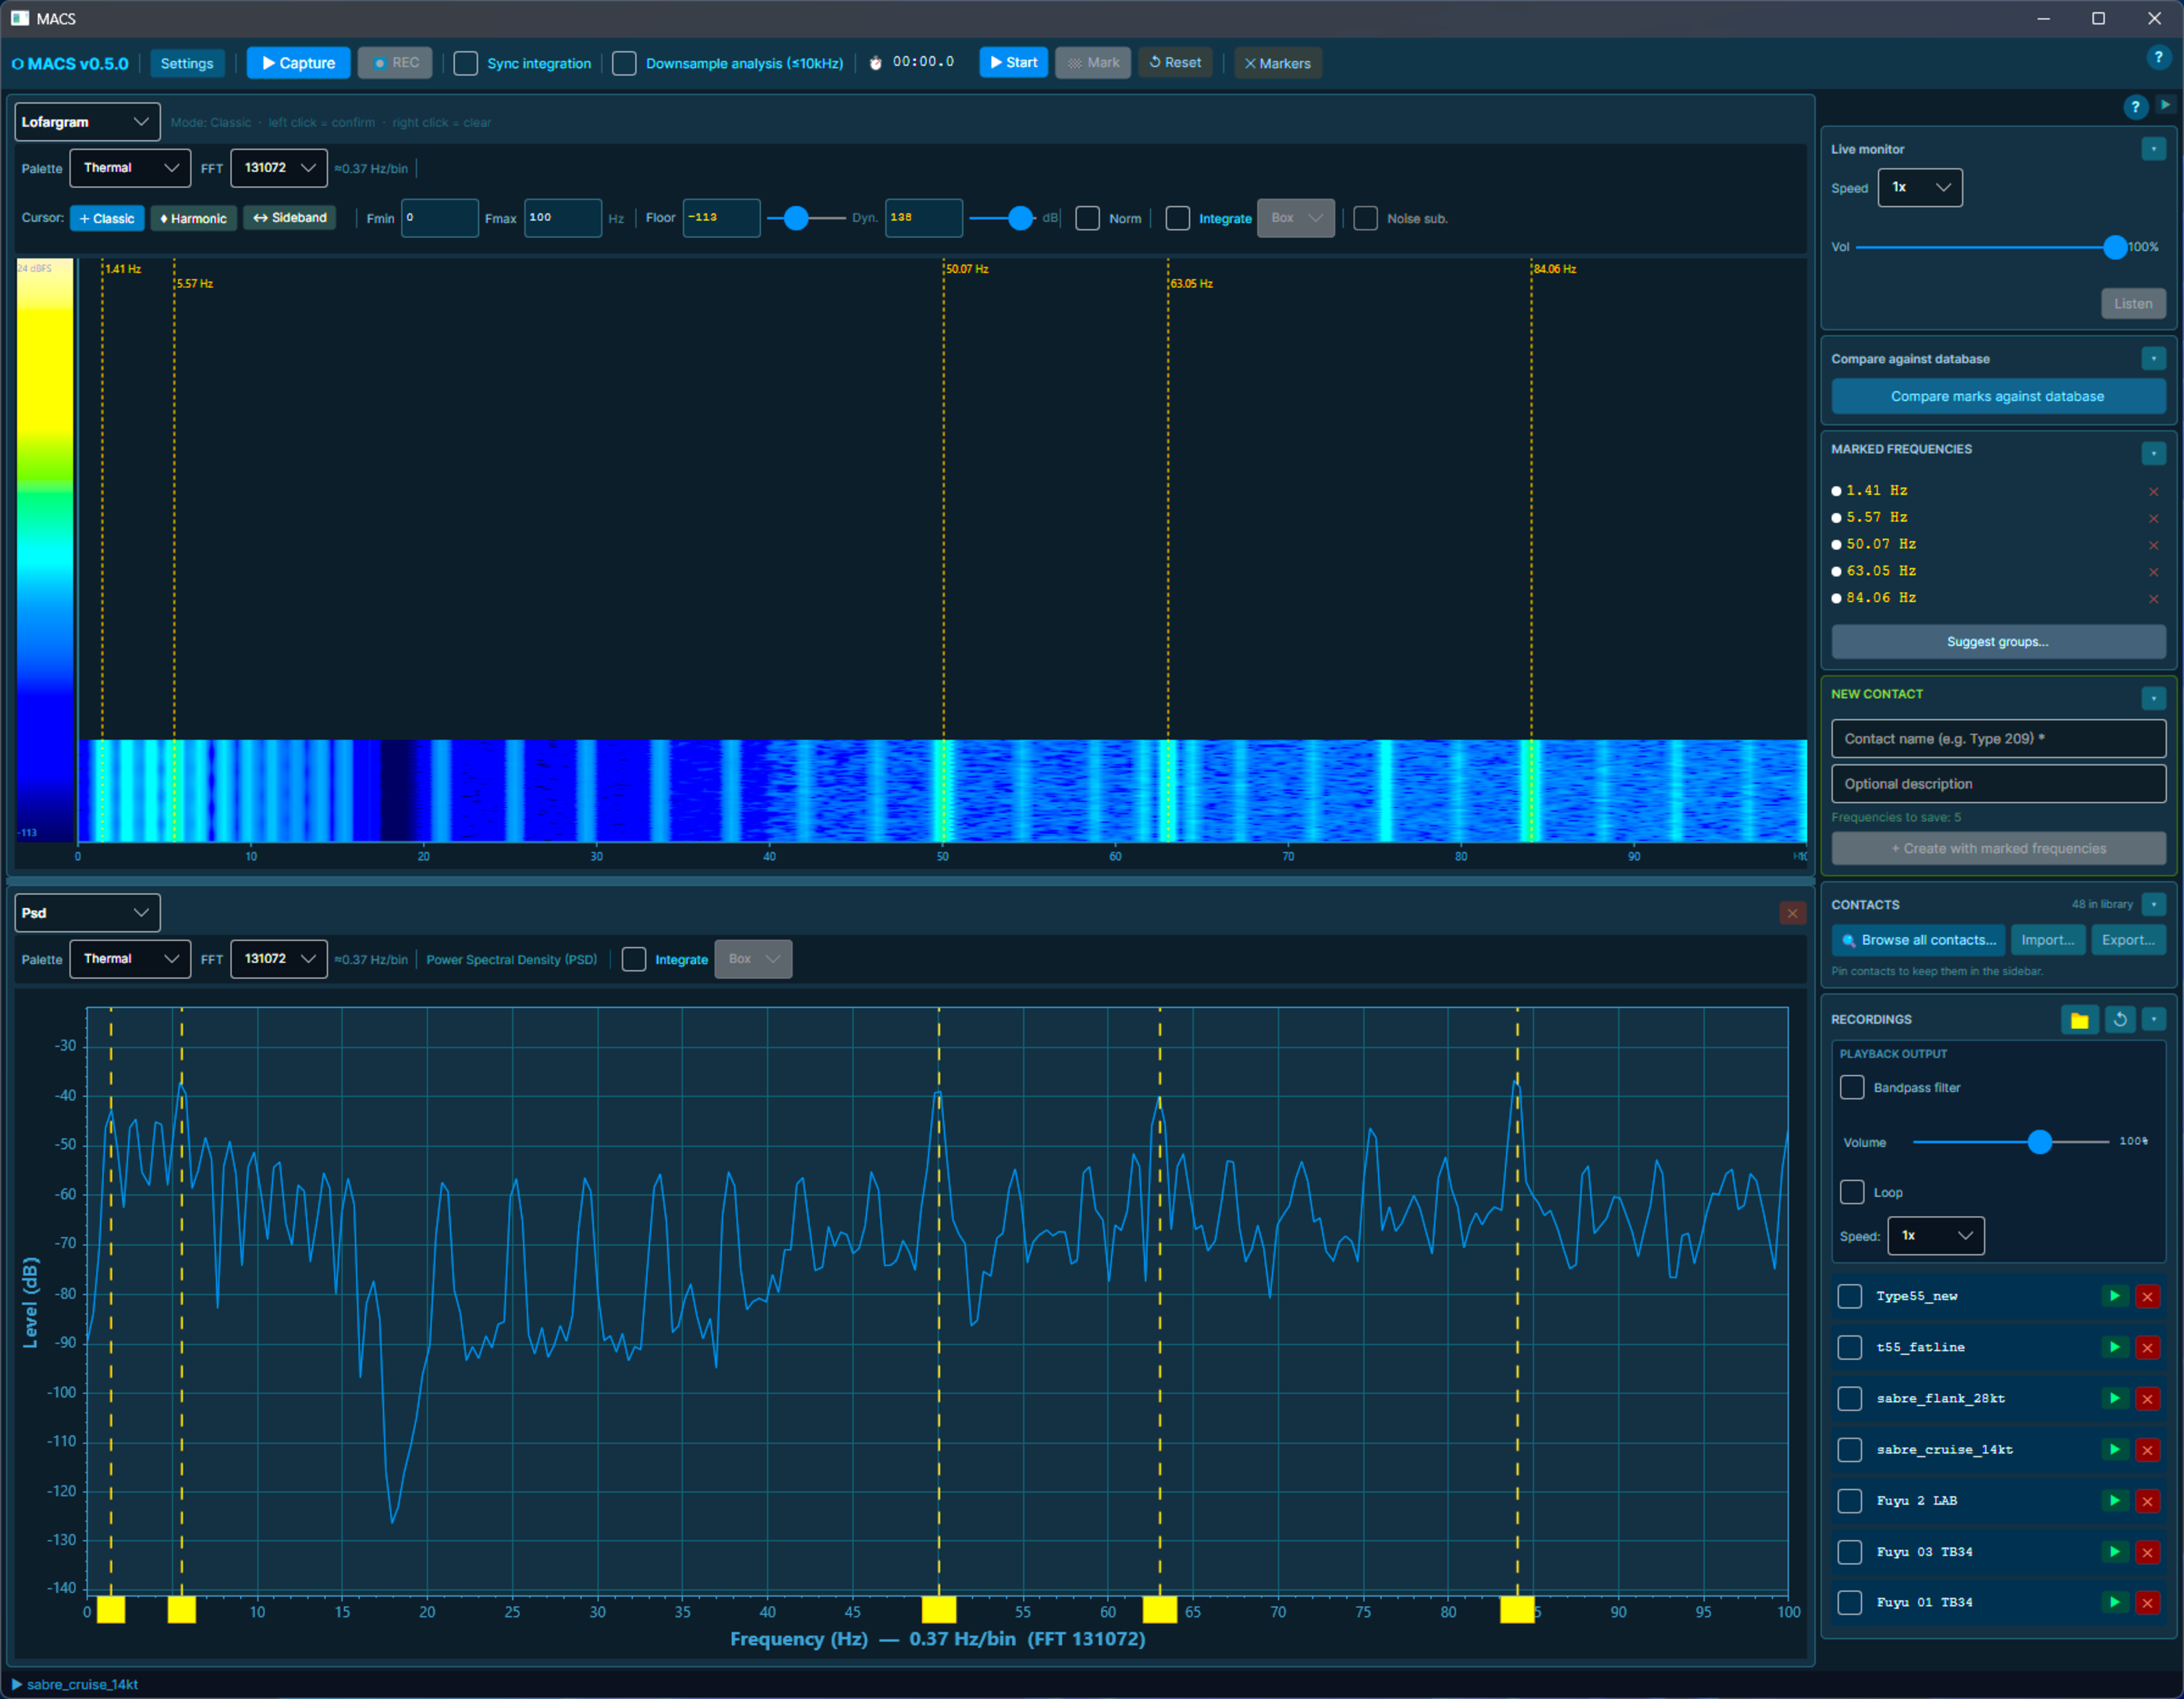
\includegraphics[width=350px]{../img/actuals/Contacts_marked.pdf}
	\caption{Contacts marked on the LOFARgram}
\end{figure}

Before clicking the \enquote{\textbf{+ Create with marked frequencies}} button fill in the \enquote{\textbf{Contact name}} and \enquote{\textbf{Optional description}} fields. On creating the new contact the Measurements Panel (Figure 8) opens where you have the opportunity to add additional measures and refine existing ones. From here you can also capture images of panels A and B for future comparison.

Contact record fields: Information

\begin{compactitem}
    \item Name: Contact identifier (vessel name or designator).
    \item Description.
    \item Class name and nation / affiliation.
    \item Classification confidence, user perception.
    \item Tag, add a tag to aid future identification, user setting
    \item Blade count: Number of propeller blades.
    \item Blade pitch: Pitch of propeller blades.
    \item Propulsion type, each checkbox opens a sub-panel allowing further detail entry
    \item Ownship when selected identifies this contact as ownship
\end{compactitem}

Contact record fields: Add measurement
\begin{compactitem}
    \item Advanced editor opens the Advanced Tonal Editor panel.
    \item Estimated speed (knots) user enters their estimations of target speed (optional)
    \item Estimated Distance (m) users distance estimation (optional)
    \item Shaft Rate (SR): Propeller shaft rotation rate in rev/s (Hz).
    \item Crankshaft Rate (CSR): Engine crankshaft rate in rev/s.
    \item Reduction factor - auto-computed $CSR / SR$. The gear reduction between engine and shaft.
    \item TPK: Turns Per Knot - auto-computed (see below). Indicates how many shaft revolutions per knot of speed.
    \item Frequency overlays: Named sets of frequency markers from the LOFARgram.
\end{compactitem}

TPK (Turns Per Knot) is computed as:

\[
TPK = \frac{SR \times 60}{Speed}
\]

This gives shaft turns per knot of vessel speed, which is a vessel-class characteristic independent of operating condition. Average TPK is computed across all measurements for a contact and shown in the contact list for quick comparison. Refinements to this calculation which include such factors as slippage are discussed in Appendix C.

The \enquote{\textbf{Measurements (n measurements)}}, \enquote{\textbf{Propulsion}} and \enquote{\textbf{Tonal library}} give access to visual representations of the contacts measurements.

To complete the process scroll to the bottom of the measurements panel and click the \enquote{\textbf{"+ Save this measurement"}} button before saving and closing the panel.

To add a measurement to an existing contact, navigate to the measurements panel (page 18) and select the \enquote{\textbf{+ Add measurement}} tab. Enter the details and then click the \enquote{\textbf{+ Save this measurement}} button before saving and closing.

\subsubsection{Advanced Tonal Editor panel and Grouping}
\textcolor{commentGreen}{*** WIP ***}

\subsubsection{Overlays}
\textcolor{commentGreen}{*** WIP May Not Be Needed ***}

Overlays let you annotate the LOFARgram with frequency markers that are saved to the contact database.

Overlay controls

\begin{compactitem}
    \item \textbf{New overlay:} Creates a new named overlay (associated with a contact).
    \item \textbf{Colour picker:} Sets the display colour for the selected overlay.
    \item \textbf{Error band:} Adds $\pm$ frequency uncertainty bars around each marker.
    \item \textbf{Line width:} Controls marker line thickness in pixels.
    \item \textbf{Cursor mode colouring:} Colours each line by the cursor mode that created it (Single /Harmonic /Resonance each get a distinct colour), overriding the overlay colour.
\end{compactitem}

Each frequency point stores its Hz value and the cursor mode used to capture it. This means the database records not just where the line is, but how it was identified: as a single tonal, a harmonic fundamental, or a resonance line.

\subsection{Contact Matching}
\textcolor{commentGreen}{*** WIP ***}

The central purpose of the database is to enable the user to classify and, potentially identify, an unknown contact. It stands to reason that in order to do this the user must have added contacts and measures to the database in order for the matching system to work.

The basic workflow is:

\begin{compactenum}
    \item For your unknown contact mark significant tonals, for instance, but not exclusively: SR, BR, CSR and electrical mains.
    \item Click the \enquote{\textbf{Compare marks against database}} in the compare against database sub-panel.
    \item In the \enquote{\textbf{Comparison results}} panel enter any additional information you may have in the \enquote{\textbf{Target known details}} fields (Figure 10 - Green Boxes).
    \item If no matches reach the partial or pass criteria adjust the tolerance setting to allow for variation in accuracy in placing markers. Too broad a tolerance will cause more misidentifications which will have to be discounted by observation (Figure 10 - Red Box)
    \item In an ideal situation you will end up with a single match (Figure 11) although it is more likely that you will have more than one and several partials.
\end{compactenum}

\begin{faintquote}
    The contact database has a lot of hidden content and features, this section is a quick overview of the functionality offered. A detailed walk through of creating, managing and matching contacts is given in the Illustrated Examples section.
\end{faintquote}

\begin{figure}[ht]
	\centering
	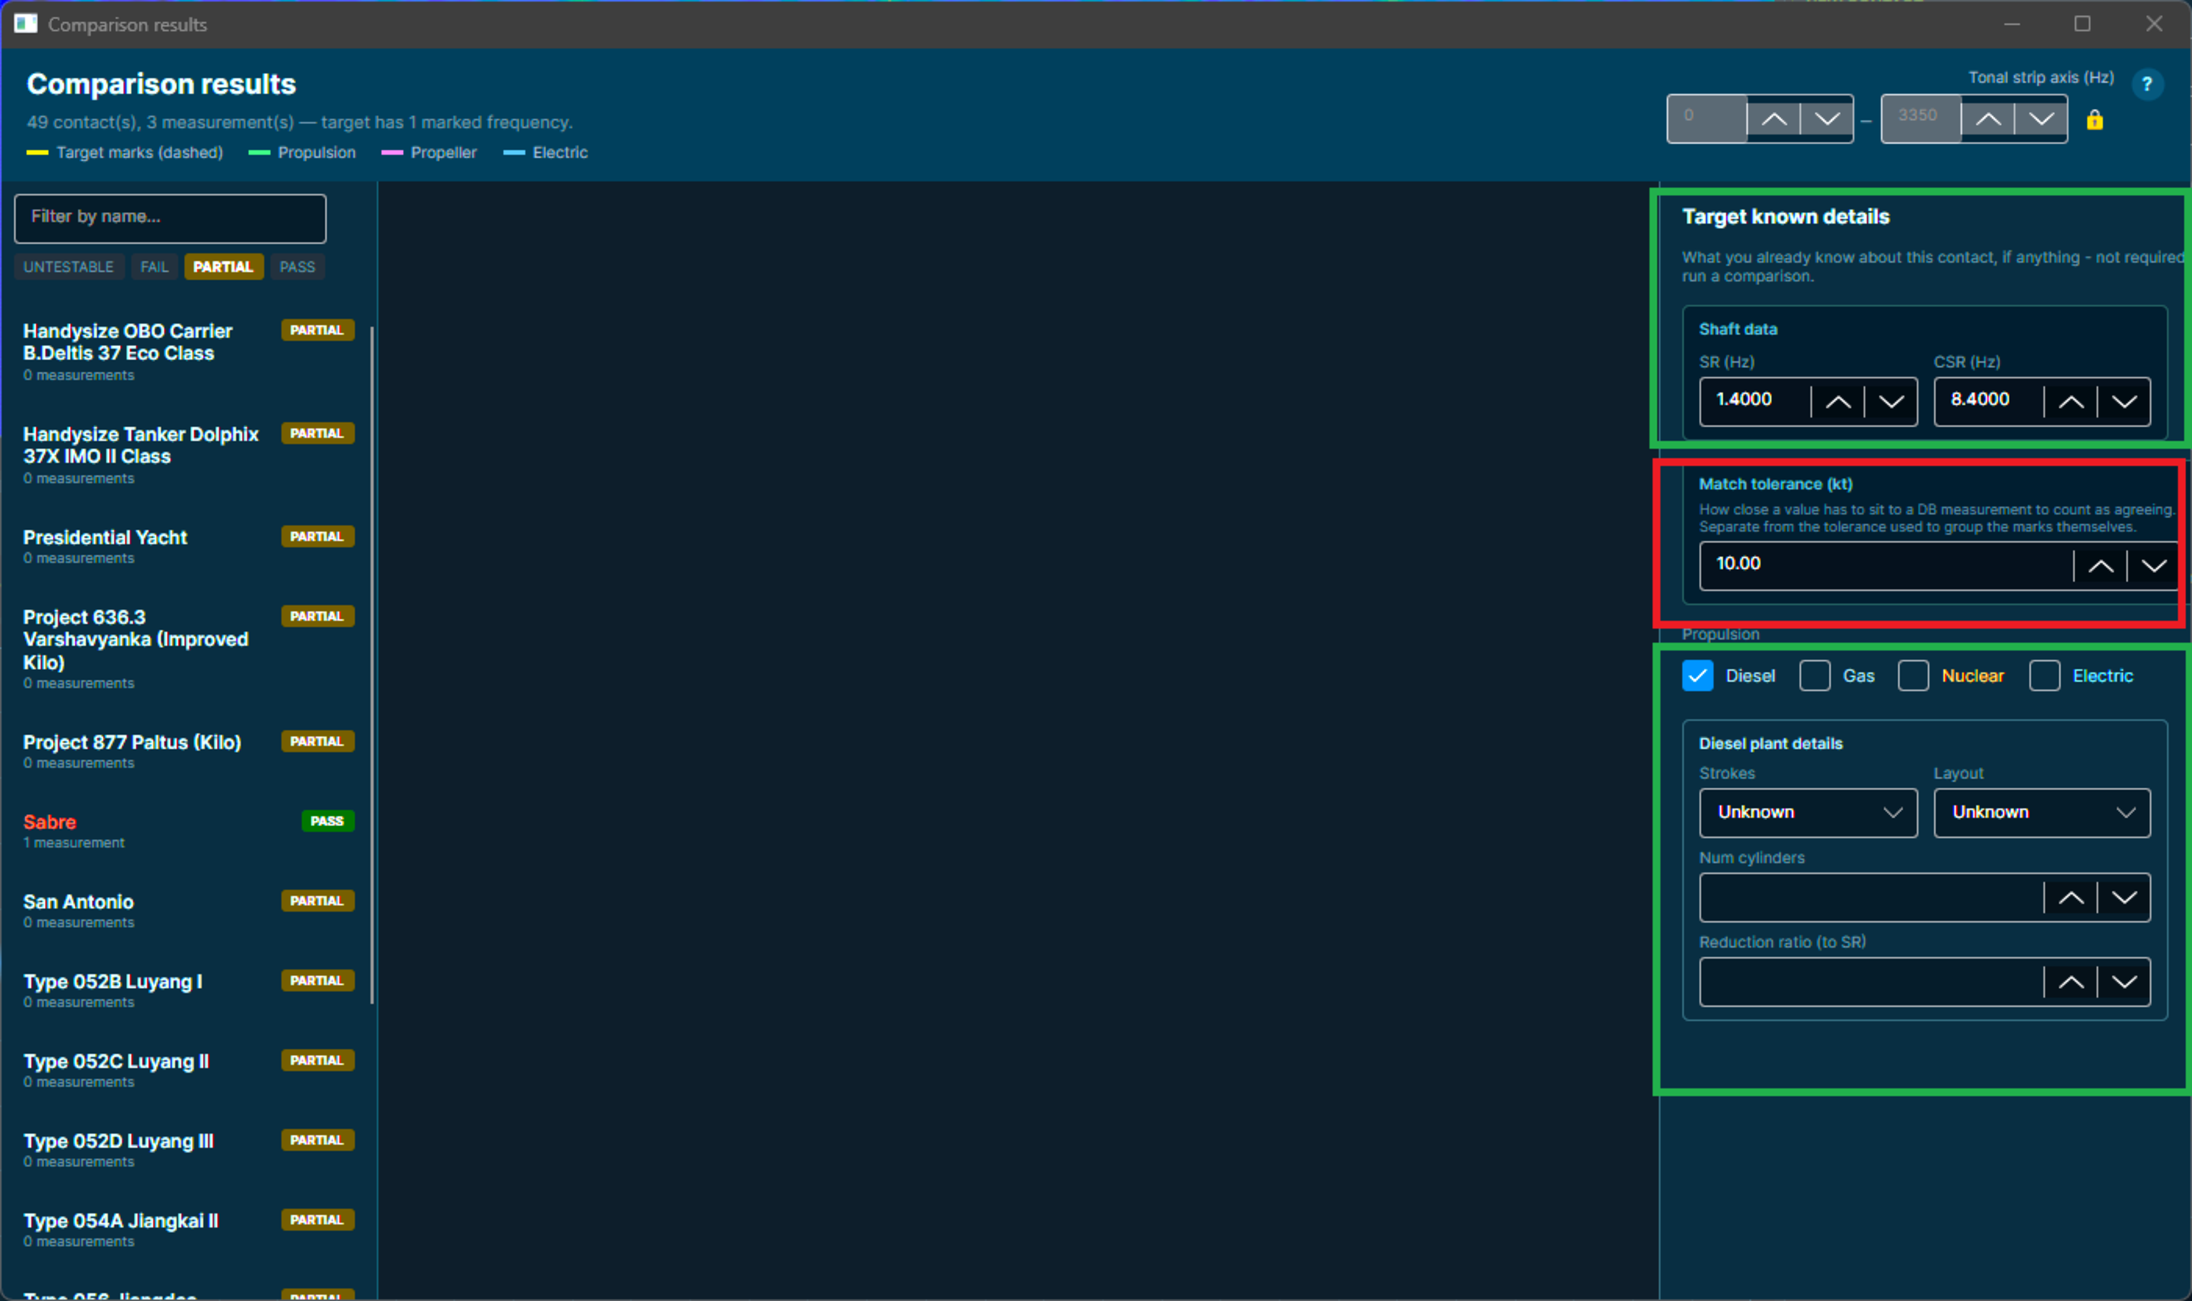
\includegraphics[width=350px]{../img/actuals/Contact_01.pdf}
	\caption{Partial Contacts}
\end{figure}

\begin{figure}[ht]
	\centering
	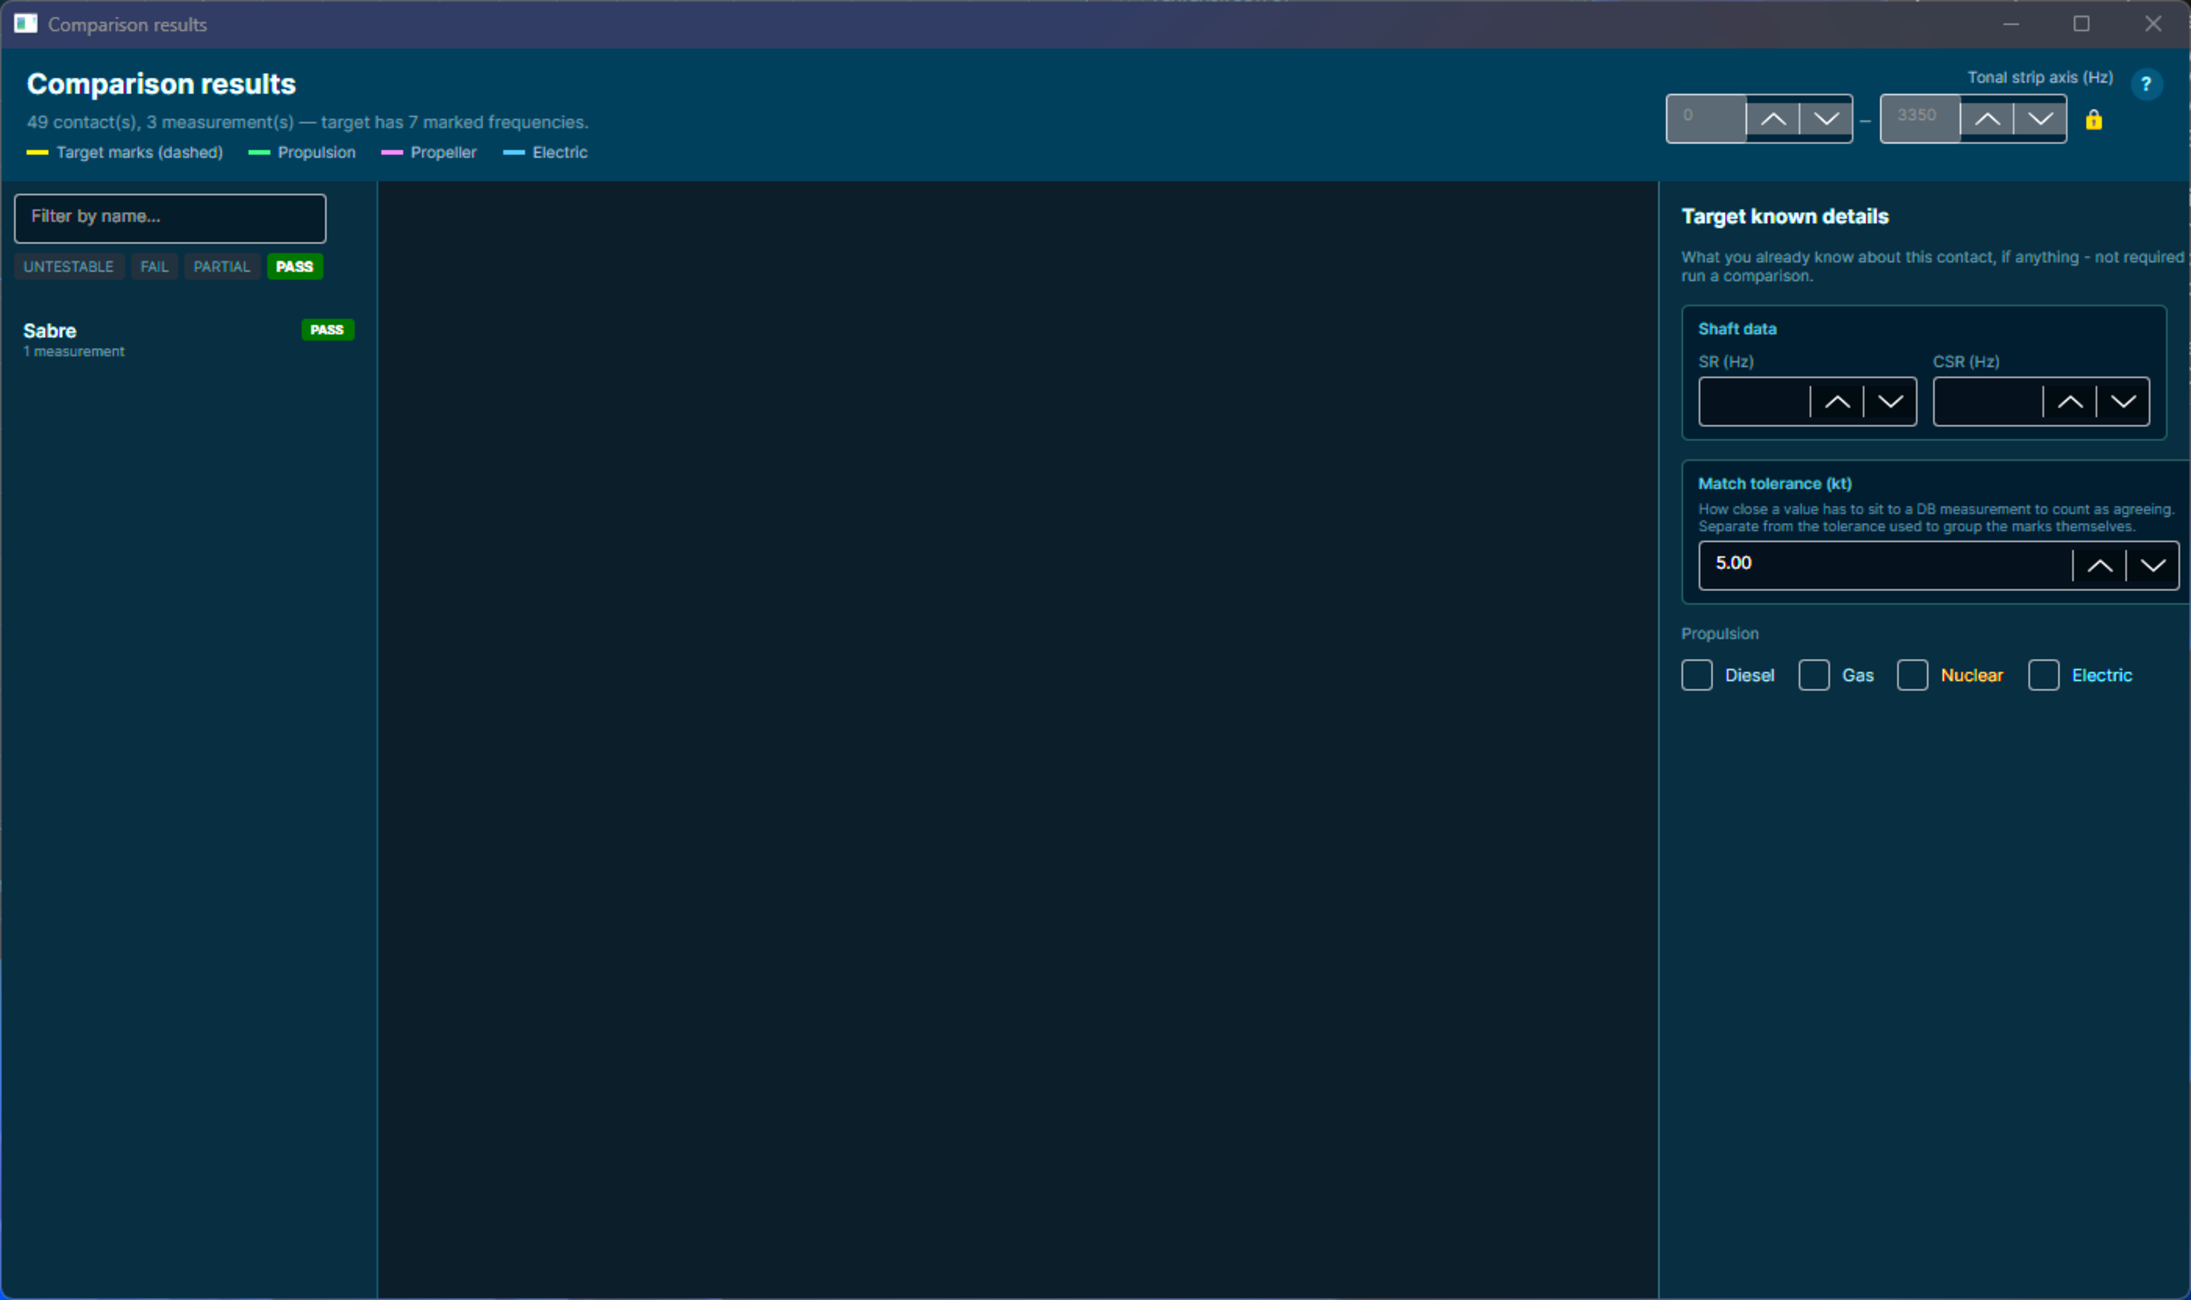
\includegraphics[width=350px]{../img/actuals/Contact_02.pdf}
	\caption{A Single Match}
\end{figure}

\subsubsection{Live Monitor}
\textcolor{commentGreen}{*** WIP ***}

%\FloatBarrier
%\pagebreak
\clearpage


\section{SONAR and Sound Analysis an Introduction}

\subsection{Background}

For submariners, the ability to detect the presence of surface ships and other submarines while remaining undetected is a matter of life and death. To achieve this, passive SONAR detection techniques have been developed to detect, classify, and determine target speed based on noise emissions. Often, detection is made harder when the signal from the ship is lost in background noise. This can occur when the marine environment is particularly noisy and/or when the ship is distant from the submarine. In order to maintain contact with a target vessel, detection must rely on some form of signal processing to enhance the acoustic signature of the ship and reduce the impact of the background noise in the sonar signal.

Remarkably, the developers of MNW have included sophisticated in-game representations of the principal components that make up the core of the detection and classification tools. These tools can only be representative of those actually used as most are classified secret by navies around the world; though, it is surprising how much is available in the public domain. Some key references are listed in the \hyperref[sec:References]{references section}. The developers have set an ambitious target of achieving as near-realistic sound modelling and propagation as is possible for the capabilities of a reasonably spec'd PC with a modern GPU. Using GPU ray-tracing capabilities, the mechanics of sound movement in water are accurately modelled. For those with long memories you will be familiar with rudimentary versions of these tools in submarine simulations such as EA's Sub Command and Black Bean's Dangerous Waters.

The process of capturing, analysing, and final classification of a target is shown in Figure 12. This workflow uses several processes which are explained below. A more detailed discussion is provided in \hyperref[sec:Appendix_B]{Appendix B}. However, for a player of MNW, the information provided in this section provides a sufficient understanding of what MACS and the game's systems are telling you.

\begin{figure}[h]
    \centering
    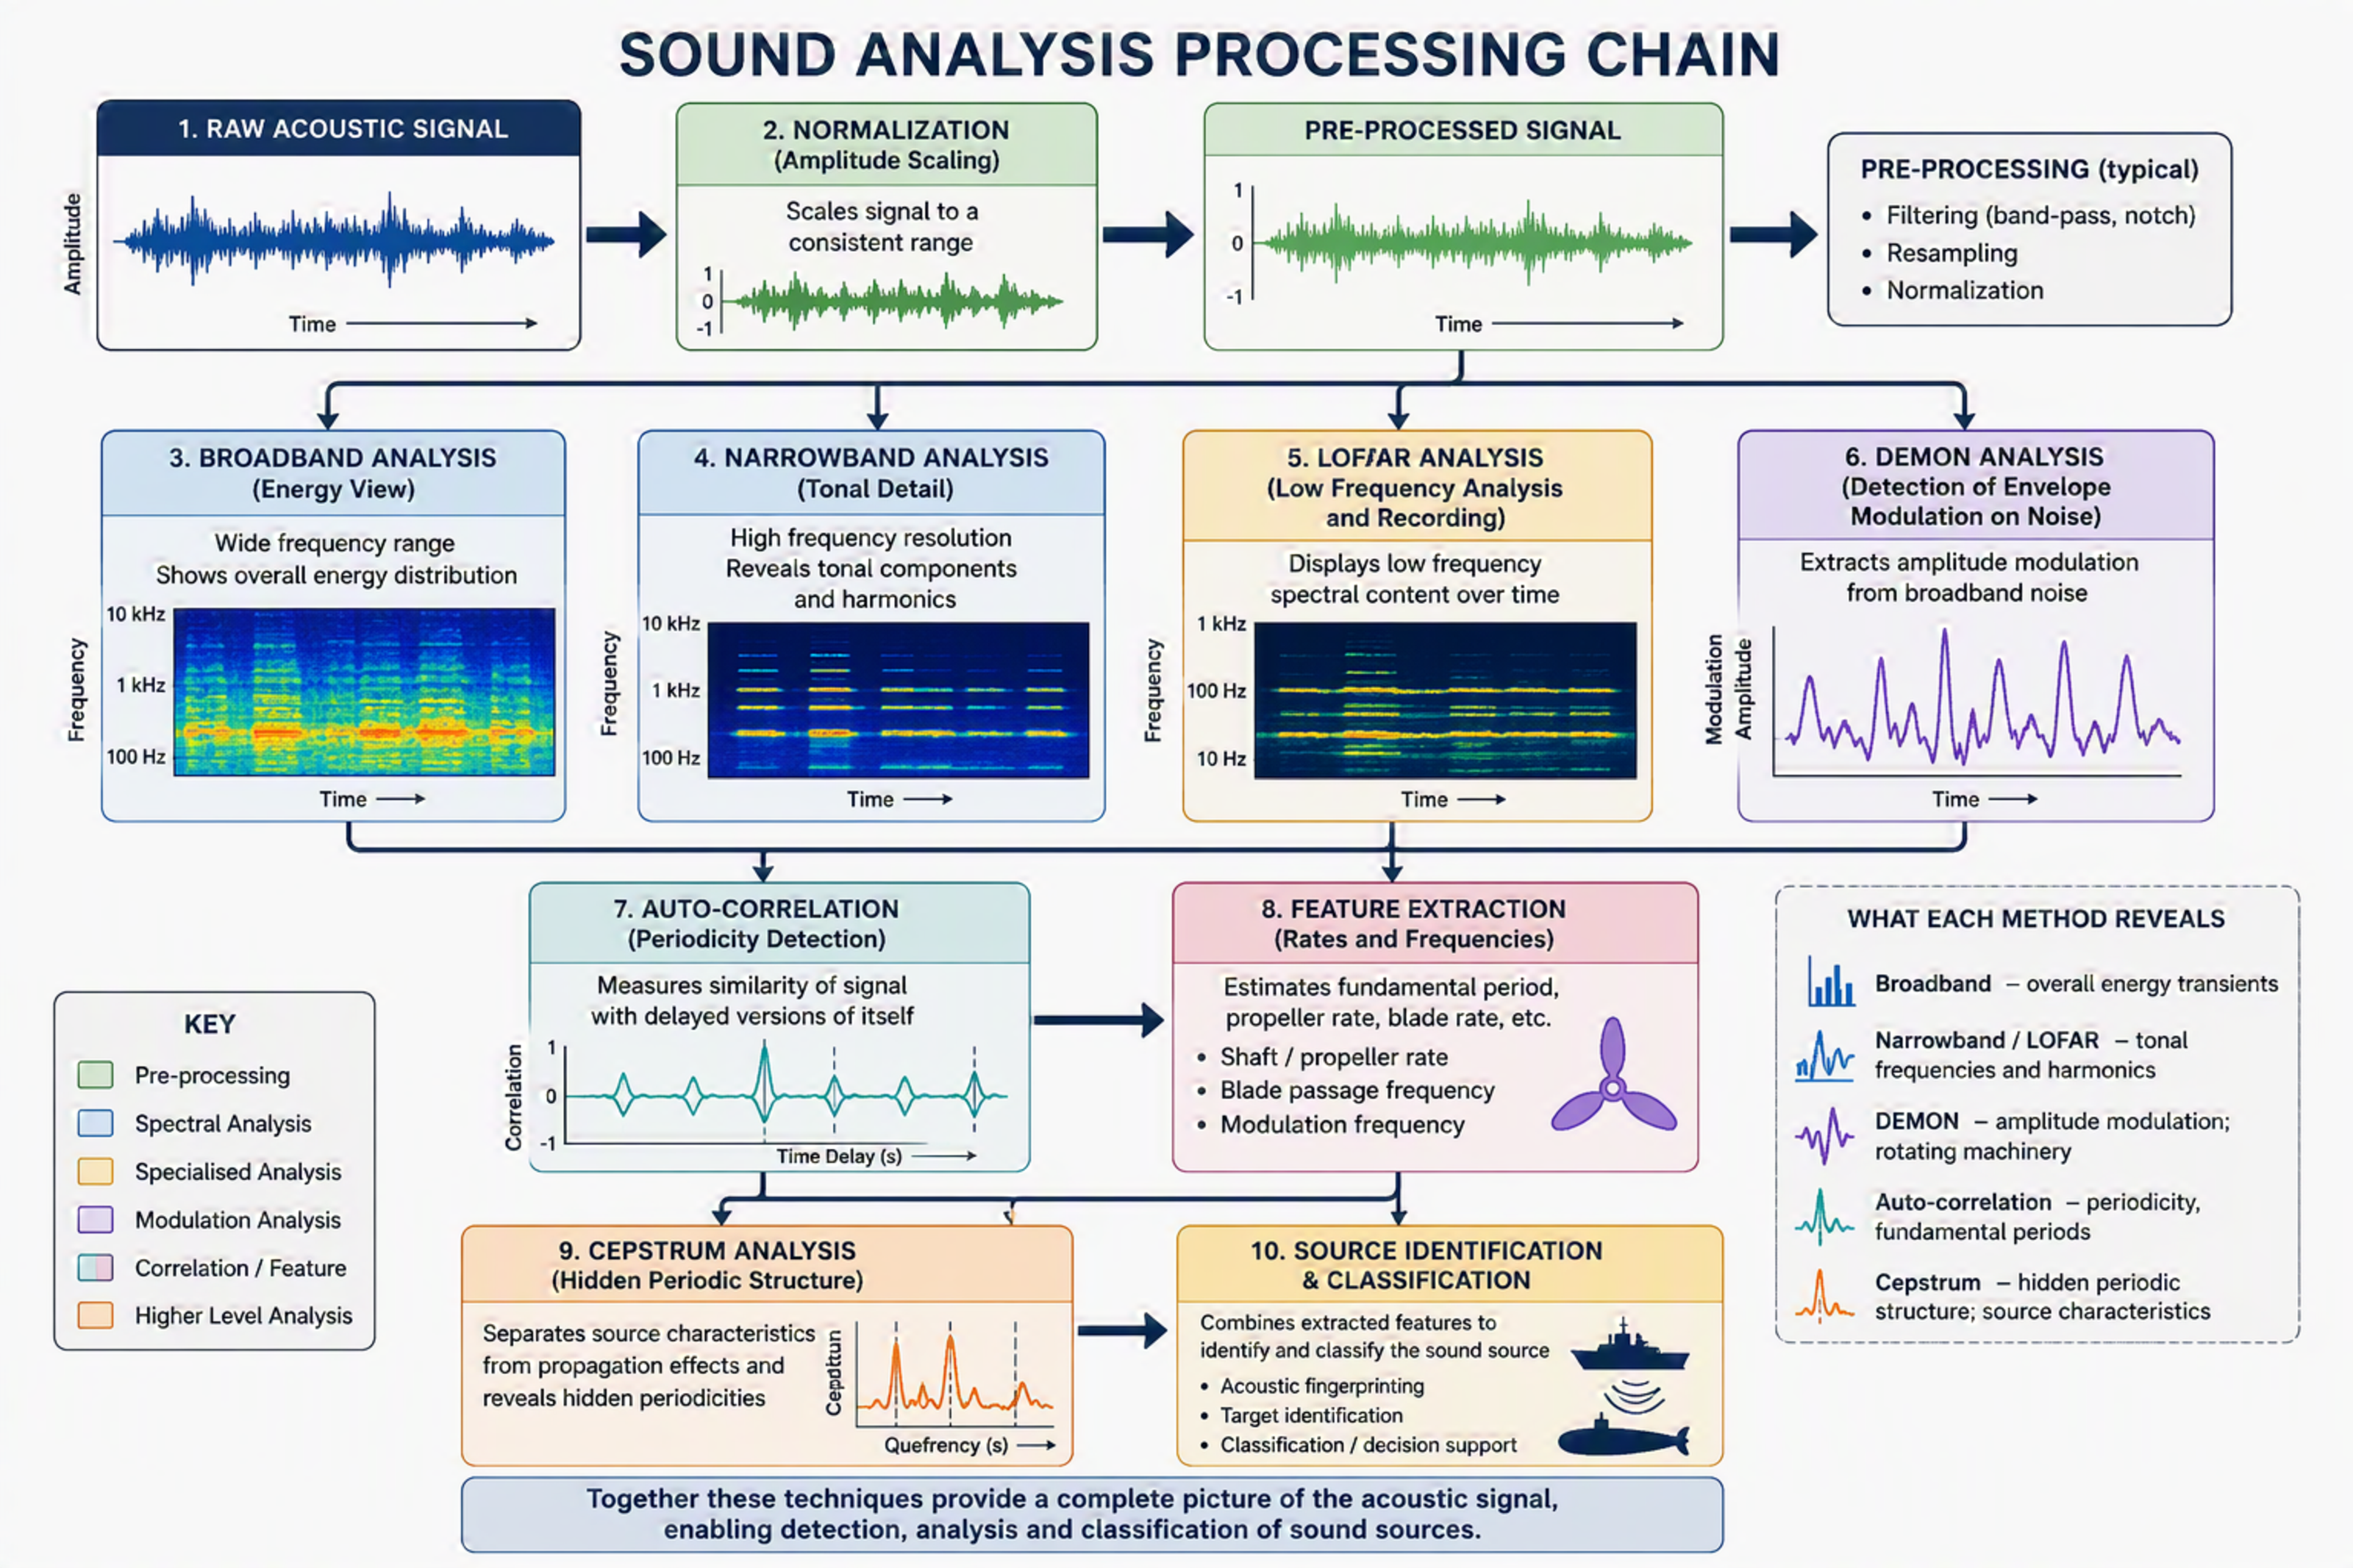
\includegraphics[width=\linewidth]{../img/actuals/sound_workflow.pdf}
    \caption{Sound analysis workflow}
\end{figure}

When MACS is used in conjunction with MNW as designed, the sound has undergone some processing in game so it can be argued that pre-processing is shared between MNW and MACS in this case.

\begin{faintquote}
    Sound analysis is the process of examining acoustic signals to extract useful information about their source, characteristics, and behaviour. Sound signals are often complex, containing multiple frequency components, background noise, and transient events. To understand these signals effectively, a range of signal processing techniques is used.
\end{faintquote}

\subsection{Broadband and Narrowband}

Broadband and narrowband analysis are complementary ways of processing the acoustic energy received by a submarine's sensors. A submarine hunting a target will typically use both methods because each provides different information. In MNW, your principal receivers of sound energy are the bow array (LAB), the flank arrays (WAA), and the two towed arrays (TA), TB34 and TB29A. Broadband analysis examines sound energy across a wide range of frequencies. It focuses on overall acoustic energy rather than specific discrete tones. Broadband is where you will often first see a contact, although this is not always the case. Narrowband analysis, on the other hand, uses finer frequency resolution to reveal detailed spectral features such as harmonics and tonal components produced by machinery, propeller blade rates, or engine harmonics. It does this by applying a Fourier Transform (FT) transforming the sound from a time based domain to a frequency domain (\hyperref[sec:Appendix_B]{Appendix B}). These frequencies are displayed as discrete tonal lines which can often be an identifying fingerprint for the contact.

\textbf{Broadband Strengths}
\begin{compactitem}
    \item \textbf{Long-range detection:} Often provides a first indication of a contact because it collects energy over a wide frequency range.
    \item \textbf{Good against noisy targets:} Effective when a target generates substantial broadband noise from propulsion or hydrodynamic flow.
    \item \textbf{Rapid contact detection:} Useful for searching large areas and finding contacts quickly.
    \item \textbf{Works when tonal lines are weak or absent:} Can detect targets whose machinery tones are masked or difficult to resolve.
\end{compactitem}

\textbf{Broadband Weaknesses}
\begin{compactitem}
    \item \textbf{Limited classification capability:} Indicates that a contact exists, but provides little information about what it is.
    \item \textbf{Vulnerable to environmental noise:} Shipping, sea state, and biologics can create broadband noise that causes false or ambiguous detections.
    \item \textbf{Less precise tracking:} Bearing estimates and contact characterization may be less accurate than narrowband methods.
\end{compactitem}

\textbf{Narrowband Strengths}
\begin{compactitem}
    \item \textbf{Excellent classification and identification:} Tonal patterns can reveal target type and sometimes specific class.
    \item \textbf{Supports tracking:} Stable tones allow accurate bearing tracking over time.
    \item \textbf{Useful against quiet contacts:} Even very quiet submarines may produce detectable tonal signatures.
    \item \textbf{Provides target motion clues:} Changes in tonal frequencies can support Doppler analysis and target speed estimation.
\end{compactitem}

\textbf{Narrowband Weaknesses}
\begin{compactitem}
    \item \textbf{Requires strong, resolvable tonal lines:} If the target is extremely quiet or its tonals are masked, analysis becomes difficult.
    \item \textbf{More susceptible to frequency instability:} Manoeuvering, environmental effects, and machinery changes can complicate interpretation.
    \item \textbf{Generally less effective as an initial search tool:} It often requires an already-established contact bearing.
\end{compactitem}

Imagine a submarine is listening for another submarine transiting at moderate speed. The target's propeller, machinery, flow noise, and other sources create a broad spectrum of noise. Broadband processing may detect a rise in acoustic energy from a particular bearing, suggesting a contact, the operator might see a contact emerge from the background noise even before any specific identifying features are apparent. After broadband analysis detects a contact, operators switch attention to narrowband displays. They may observe a set of stable tones at particular frequencies. Those frequencies can be compared to intelligence databases, acoustic signatures, notebooks and experience.

A weak broadband signal does not always mean weak spectral features. From a broadband point of view a very faint vessel at 50Hz broadband is merged with contributions from a much wider frequency band. This means that BB is dealing with background noise from all of that frequency range. So the signal to noise ration (SNR) is very low or indiscernible on the broadband screen. Narrow band on the other hand looks at how much energy is available at each frequency band (Fourier Transform) and bins them in bands. So in the frequency domain the 50hz signal will stand out and this is reinforced by persistence of the signal over time.

Where broadband may give an early detection is for a good SNR and when enough energy is being pumped into the water. In this case broadband is very effective. A source with strong broadband noise might appear BB-first. A comparatively quiet source with prominent persistent machinery/propulsion tonals can potentially become apparent in NB/LOFAR without an obvious BB signature.

\begin{faintquote}
    In modern anti-submarine warfare, classifiers do not choose one over the other; they use them together. Narrowband data is used to classify the specific ship type via its engine noise, while broadband data (both passive flow noise and active echoes) is used to map the target's size, speed, and exact spatial position.
\end{faintquote}

\subsection{Normalization}

Before advanced analysis is performed, signals are often subjected to normalisation. Normalisation is a statistical technique that scales the signal amplitude to a consistent range. A well-known and commonly used method is the Z-score however there are many other strategies available. The effect is to reduce the influence of recording-level variations, allowing meaningful comparisons between different measurements. This preprocessing step improves the robustness of subsequent analysis techniques and ensures that results reflect the signal characteristics rather than differences in recording conditions. The approach used by MACS to normalise data is explained in \hyperref[sec:Appendix_B]{Appendix B}.

\subsection{LOFAR (Low Frequency Analysis and Recording)}

In underwater acoustics and sonar applications, LOFAR is a fundamental technique. It is a passive narrowband sonar signal-processing technique which displays the spectral content of low-frequency signals over time. These tonal signatures can act as acoustic fingerprints, helping to detect, classify, and sometimes identify ships and submarines from the sounds they radiate into the water. Narrowband is used because:

\begin{compactitem}
    \item \textbf{Extreme Long Range: }Low-frequency narrowband signals can travel very long distances through the ocean without losing energy (\href{https://www.youtube.com/watch?v=sP85wUcg6_A}{YouTube}), allowing for early detection of distant threats.
    \item \textbf{High Signal-to-Noise Ratio: }By filtering out background ocean noise and focusing strictly on ultra-thin frequency bands, LOFAR can extract faint mechanical signals that are otherwise invisible to the naked ear or broadband sensors
\end{compactitem}

\begin{faintquote}
    Below roughly 100 Hz, ocean conditions can allow very efficient propagation with relatively low energy loss, which is why low-frequency sound may travel enormous distances. But the low-frequency ocean is also a very noisy place, with shipping, machinery, environmental noise and other sources contributing substantial energy. That is exactly why "travels further" does not necessarily mean "easier to detect". Sonar performance ultimately depends on received SNR, not merely propagation distance.
\end{faintquote}

Sound received by the SONAR arrays is transformed into a "frequency domain" which shows how much energy exists for every single frequency. This is typically done using a FFT (Fast Fourier Transform). FFT is a mathematical algorithm which allows the huge amount of information contained in the sound data to be analysed quickly. The result is displayed as a LOFARgram (a time-frequency spectrogram), where persistent frequency components appear as lines. This is useful because ships and submarines generate characteristic underwater noise from:

\begin{compactitem}
    \item Main engines and generators
    \item Gearboxes and pumps
    \item Propeller blade rotation and cavitation
\end{compactitem}

These sources produce distinctive frequency components. By examining the pattern of tonal lines in a LOFAR display, operators can distinguish different vessel types and, specific classes of ships and, sometimes, individual ships. To summarize, NB analysis describes the type of spectral analysis, i.e. high frequency resolution separating spectral components that are very close together to reveal distinct tonals. LOFAR is an application and presentation of a narrowband analysis typically focussing on the lower-frequency part of the spectrum as this is where many diagnostic tonals are, e.g. shaft rate, blade rate etc. So, to be concrete NB refers to spectral resolution / bandwidth and LOFAR describes the signal-processing and visualisation techniques.

\begin{faintquote}
    In summary, LOFAR is a passive sonar technique that converts underwater sounds into a time-frequency display, enabling operators to detect ships and identify them from their unique acoustic signatures. LOFAR is often paired with DEMON analysis.
\end{faintquote}

\subsection{DEMON (Detection of Envelope Modulation on Noise)}

DEMON processing focuses on amplitude modulations (AM) present within broadband noise. In simple terms, it means taking a steady, continuous wave and making it rhythmically louder and quieter over time. For example, the rotation of a ship's propeller produces periodic fluctuations in noise levels at characteristic frequencies, such as:

\begin{compactitem}
    \item Shaft rotation frequency
    \item Blade-passing frequency or Blade Rate(BR)  
\end{compactitem}

DEMON extracts the amplitude envelope of the received noise and analyses it in the frequency domain. The resulting spectrum reveals peaks corresponding to the vessel's mechanical and propeller characteristics, which can be used for identification and classification. This is useful because:

\begin{compactitem}
    \item Enhances weak periodic signatures hidden in broadband noise.
    \item Helps estimate propeller speed, number of blades, and other target features.
    \item Widely used in passive sonar target detection and classification systems.
\end{compactitem}

\begin{faintquote}
   \textbf{LOFAR} emphasizes the ship's frequency spectrum (machinery and tonal components). \textbf{DEMON} is useful for extracting propeller-related modulation and blade-rate information. 
\end{faintquote}

\subsection{Cepstrum and Auto-correlation}

\textbf{Cepstrum} analysis is a powerful signal-processing technique used in acoustics. Developed to reveal hidden periodic structures in the frequency spectrum of a signal, it is particularly effective for separating source characteristics from propagation effects.

The basic idea behind cepstrum analysis is to detect echoes, repeating patterns, or modulation effects within a signal. In many real-world applications, a recorded signal is not simply a direct waveform but rather a combination of a source signal and the influence of the medium or system through which it passes. For example, in sonar, received energy may contain reflections from multiple surfaces, and in machinery monitoring, vibration signals are influenced by rotating components and gears. Cepstrum analysis helps separate these effects and identify underlying periodicities.

\textbf{Auto-correlation} is commonly used to detect periodic acoustic signatures produced by ships, submarines, and marine machinery. Many sources generate signals that repeat at regular intervals, such as rotating propellers, diesel engines, pumps, and gear systems. The periodic nature of these sounds produces corresponding peaks in the auto-correlation function. The spacing between peaks indicates the repetition period, from which the rotational speed or blade-passage frequency can be estimated.

In simple terms, auto-correlation measures how similar a signal is to a delayed version of itself. By comparing the signal with progressively shifted copies, it becomes possible to detect hidden periodicities and determine whether certain features repeat over time.

For example, consider a vessel whose propeller completes two revolutions per second. If the acoustic signal generated by the propeller repeats every 0.5 seconds, the auto-correlation function will exhibit peaks separated by approximately 0.5 seconds. The analyst can use these peaks to determine the underlying mechanical characteristics of the vessel and potentially aid in classification and tracking.

You will find more details about Cepstrum and auto-correlation in \hyperref[sec:Appendix_B]{Appendix B}.

\pagebreak

\section{SONAR Classification 101 and MACS Workflow}

\subsection{What you will learn in this section}

\begin{compactenum}
    \item How to understand and use LOFAR and DEMON.
    \item How calculate propeller shaft and blade rates (SR BR) to provide signature information and an estimate of the vessels speed.
    \item Understand what the different diesel engine configurations are including calculating Individual Cylinder Firing Rate (ICFR), Crankshaft Rate (CSR), Engine Firing Rate (EFR) and determining the number of cylinders.
    \item How to recognise harmonics, sidebands and reduction ratios and understand how a contact can be classified from these signatures.
    \item How to recognise additional information and distinguish if these signatures are engine or shaft related, or are fixed features such as electrical mains.
\end{compactenum}

\textbf{Before attempting the examples in Section 7, you should read and have a reasonable grasp of this section.}

\begin{faintquote}
    This section introduces some of the basic mathematics behind SONAR analysis all of which is simple arithmetic and can be done with a calculator. The deep mathematics behind Fourier Transforms and cepstrum analysis is more complicated but you do not need knowledge at that level to enjoy MNW or use MACS. For those interested in the deeper detail you will find it in Appendix B.
\end{faintquote}

Although it is tempting to dive in to the powerful tools available in MACS you should, at first, take a step back as a useful amount of data can be collected by simply listening. After an initial assessment you will be working primarily with the MACS LOFAR and DEMON screens. If these are new names for you, read Section 2 \textbf{SONAR and Sound Analysis an Introduction}. You may also use the CEPSTRUM and Auto-Correlation (ACF) features explained below and in Appendix B. 

A LOFARgram is a visual representation of the LOFAR analysis, it is generally not something an inexperienced user can interpret just by looking at it. Sonar analysts are not simply spotting lines, they are using their knowledge of how machinery generates frequencies, how they relate mathematically to one another and to specific machinery. When you are trying to understand what you are hearing think of yourself as a detective. Observe patterns, form hypotheses, test them mathematically and look for evidence that supports or disproves them.

\begin{faintquote}
    As with any good hypothesis the best is usually the one that explains the greatest number of outcomes with the fewest assumptions (Occam).
\end{faintquote}

The LOFARgram is your primary tool. The display is a waterfall of the sound spectrum, with brightness indicating signal strength. In MACS, time flows from bottom to top and frequency runs left to right on the horizontal (\textit{x}) axis; often called the frequency domain.

You are looking for: \textbf{Tonals (narrowband lines)} These appear as bright \textbf{vertical lines}, a continuous stripe at a fixed frequency persisting as time scrolls past. Every significant machine on a vessel produces a characteristic set of tonals: main engine, generators, pumps, turbines. Although, they may not always be visible. The most common cause of poor broadband resolution is poor signal to noise ratio and orientation to the target. The LAB has a blind spot directly astern and the towed arrays have blind spots directly ahead.

The DEMON display is your primary analysis tool for \textbf{propeller configuration and SR.} When a marine vessel travels through water, the rotating propeller blades can create pockets of low pressure forming tiny vapour bubbles that rapidly collapse; a phenomenon known as cavitation. This collapse produces a continuous, broadband hissing noise. As the propeller rotates it causes an amplitude modulation at lower frequencies corresponding directly to the physical movement of the mechanical propulsion system. Essentially, the high-frequency cavitation acts as a "carrier wave" that is amplitude modulated (AM) by the low-frequency mechanics of the ship.

However even without cavitation, the propeller/ship can produce broadband noise whose amplitude varies periodically with shaft or blade rotation. The following lists some of these other sources.

\begin{compactitem}
    \item Non-uniform wake into the propeller. Water reaching the propeller is not uniform because the hull, appendages and shafting disturb the flow. As each blade rotates through regions of faster/slower or more turbulent inflow, its hydrodynamic loading changes. That can modulate the radiated noise at blade rate and harmonics.
    \item Blade-to-blade differences. Real propellers are not perfectly identical. Small differences in blade geometry, fouling, damage or loading can make one blade noisier than another. That can introduce modulation at shaft rate, because that distinctive blade comes round once per revolution.
    \item Turbulent boundary-layer/wake noise. Even without vapour cavitation, turbulent water interacting with the propeller and hull produces broadband pressure fluctuations. Rotation through a non-uniform turbulent field can impose periodic structure on that otherwise random broadband noise.
    \item Propeller/hull interaction. The periodically varying forces generated by the rotating propeller can interact with the stern/hull and radiate noise. This can contain shaft-rate and blade-rate periodicities.
    \item Rotating machinery. Pumps, motors, gears, bearings and other machinery can generate broadband vibration/noise whose level is periodically modulated by rotation. This isn't necessarily propeller -DEMON, but mathematically DEMON-type envelope analysis can reveal those periodicities too.
\end{compactitem}

The resulting output, often displayed as a DEMONgram, reveals distinct spectra that correspond to the vessel's unique physical traits. Sonar operators analyze these lines to identify important features of the  target. By revealing these mechanical design characteristics, the specific class, or even the individual identity, of a target submarine or surface ship can be determined with a good degree of confidence.

\begin{faintquote}
    The transition from “finding lines” to “recognising families, harmonics, and sidebands” is usually the point where a trainee starts thinking like an analyst rather than an operator.
\end{faintquote} 

The ultimate aim of a SONAR analysis is to create a "fingerprint" of the vessel under consideration. It is not necessarily to categorically identify an individual ship, although than can happen. Instead the information derived is stored in a database. This data can then be used to match future encounters and narrow down the type and classification of vessels. Over time more detail can be added refining the classification. The key diagnostic information usually sought includes:

\begin{compactitem}
    \item Engine types (diesel, turbine, electric drive)
    \item Ship propulsion fundamentals (BR, SR)
    \item Number of prepeller shafts
    \item Propeller blade counts
    \item Engine characteristics (CSR, Number of cylinders, EFR and ICFR)
    \item Gear Mesh Frequency (GMF), Gearbox arrangements and reduction ratios
    \item Electrical mains frequencies
\end{compactitem}

First though we need to understand a couple of important terms.

\subsection{What are Harmonics?}

Harmonics occur because real machinery does not produce perfectly smooth vibrations. A perfect rotating shaft would generate a pure tone at one frequency (sinusoidal) but real machinery isn't perfect it produces pulses, impacts, and uneven forces (Figure 13). Diesel engines don't apply torque smoothly, each combustion event is a pulse. A 15 Hz engine-related frequency might produce harmonics at 15, 30, 45, 60 and 75 Hz. Harmonics are always a fixed distance apart and always an integer multiplication of the fundamental, in this case 15 Hz multiplied by 2, 3, 4 etc. SONAR analysts love harmonics because whilst a single line on a LOFARgram is weak evidence, a harmonic family is powerful evidence. Sometimes the fundamental line may not be visible but can be inferred by back-counting the harmonics. MACS provides tools to do this automatically and to confirm the periodicity of suspected harmonics. The sources of the variation could be one or more of:

\begin{compactitem} 
    \item Uneven forces
    \item Multiple cylinders
    \item Gear teeth impacts
    \item Bearing imperfections
    \item Structural resonances
    \item Blade loading variations
\end{compactitem}

\begin{faintquote}
    \textbf{Why is this important}: because in our diesel engine the harmonics point back to the fundamental value (15 Hz). Even if the fundamental is weak, the harmonics may reveal it.
\end{faintquote}


\begin{figure}[ht]
	\centering
	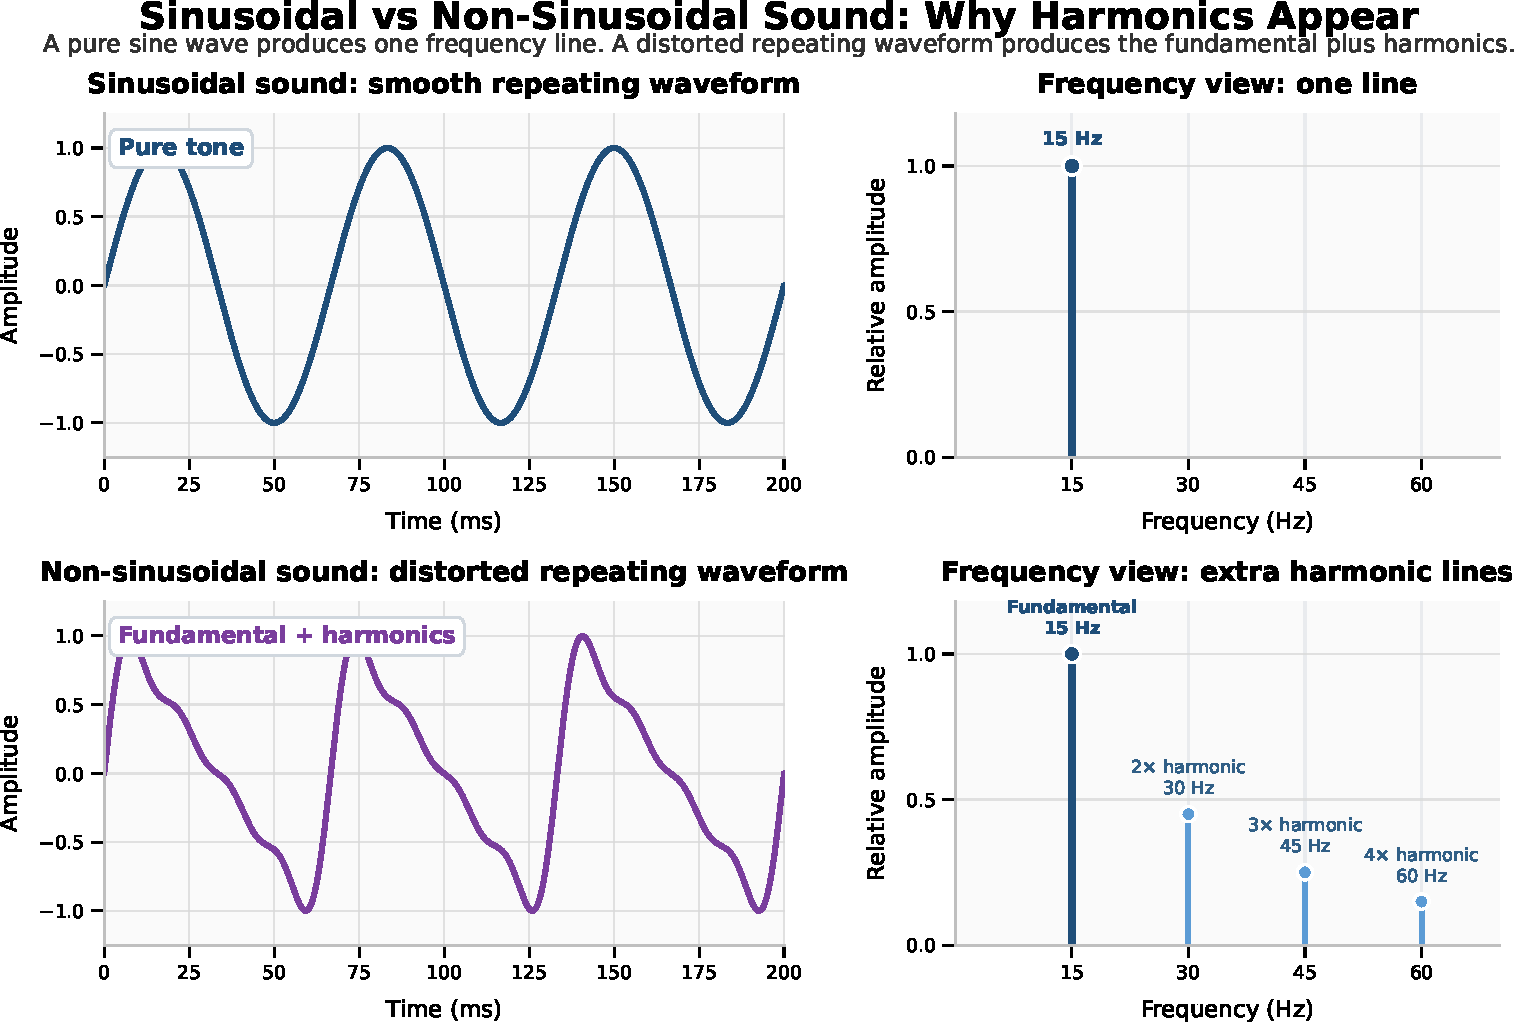
\includegraphics[width=\textwidth]{../img/actuals/sinusoidal_vs_nonsinusoidal_sound.pdf}
	\caption{Harmonics caused by sinusoidal waveform vs non-sinusoidal waveform}
\end{figure}

\subsection{What are Sidebands?}

In radio, a carrier frequency is modified by amplitude (AM) or frequency (FM), the carrier doesn't disappear, instead, additional frequencies appear on either side of it. The same occurs with machinery. An AM sideband, caused by a damaged bearing clicking once per revolution, creates a periodic rise and fall in the amplitude of the high-frequency machinery noise. AM produces exactly one pair of symmetrical sidebands $(f_c + f_m \mathrm{ \ and\ } f_c - f_m)$. In FM modulation the frequency is shifted up and down. A rotating propeller shaft might vibrate causing the carrier frequency to speed up or slow down. FM produces an infinite series of sidebands (Figure 14 Page 24) spaced at intervals of $f_m \quad (f_c \pm f_m, f_c \pm 2f_m, f_c \pm 3f_m ...)$. Suppose a gearbox produces a strong tone at 150 Hz and a propeller shaft rotates at 2.5 Hz. If the shaft causes the gearbox load to increase and decrease once per revolution, the 150 Hz gear tone is being modulated at 2.5 Hz. Instead of 150 Hz you get 145, 147.5, 150, 152.5 and 155 Hz.

In reality, targets rarely exhibit pure AM or pure FM. A propeller blade passing close to a ship's hull undergoes dynamic pressure changes simultaneously altering the amplitude of the acoustic wave (AM) and slightly shifting the phase/frequency (FM). Sonar analysts use specialized tools like DEMON processing to isolate these combined sidebands and identify the specific machinery signatures of a vessel.

\textbf{Sideband Recognition Rule:} when you spot a strong tonal:

\begin{compactenum}
    \item Find the centre frequency.
    \item Look equally above and below it. Is it symmetrical?
    \item Measure the spacing.
    \item Check whether the same spacing exists elsewhere.
    \item Look to see if the lines move together as the target vessel's speed changes
    \item Hypothesise: "Could this spacing be a shaft rate, blade rate, or engine-related rate?"
\end{compactenum}

\begin{figure}[ht]
	\centering
	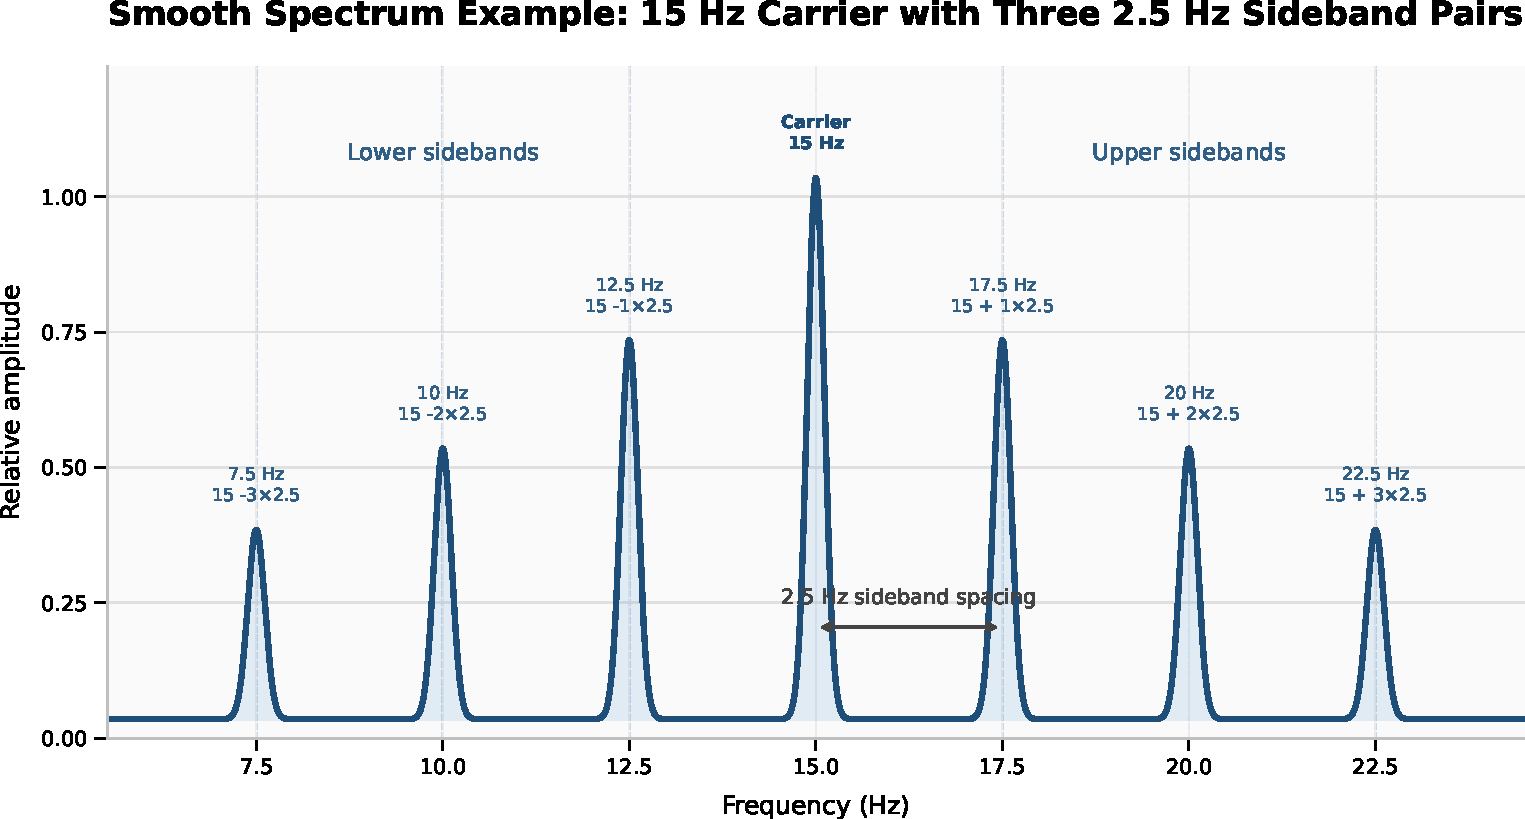
\includegraphics[width=\textwidth]{../img/actuals/sideband.pdf}
	\caption{Sidebands caused by modulation}
\end{figure}

\begin{faintquote}
    The sideband spacing is often the real clue frequently telling you more about the machinery than the large central line itself.
\end{faintquote}

\subsection{LOFARgrams - what to look for}

\begin{compactitem}
    \item \textbf{Fundamental engine frequencies} and their harmonics e.g. CSR, EFR and gear mesh.
    \item \textbf{Blade rate} = $SR \times BC$. May be visible in the 5 - 100 Hz range for surface ships although low frequency tonals are more likely to be spotted in DEMON.
    \item \textbf{Electrical mains} typically multiples of 50 or 60 Hz.
    \item \textbf{Generator harmonics} The GenSet is often an independent motor with its own rotating components producing tonals specific to it.
    \item \textbf{Broadband noise level} A vessel moving fast will show a raised broadband floor (cavitation); the entire display is brighter. A slow or quiet vessel may show almost no broadband increase, with only discrete tonals against a dark background.
    \item \textbf{Frequency drift} A tonal that slowly shifts upward or downward in frequency is Doppler-shifted, meaning the contact's radial velocity (range rate) is changing. It is accelerating, decelerating, or turning. A line that stays at a fixed frequency means the radial velocity is constant, but this says nothing about absolute range; the contact could be closing, opening, or crossing at a steady speed.
\end{compactitem}

\textbf{Practical tips:}
\begin{compactitem}
    \item Zoom Fmin / Fmax around a suspected harmonic family to check spacing.
    \item Enable normalisation to make weak tonals visible against a noisy floor.
    \item Use noise reference subtraction if own-ship noise is masking the target.
    \item Use harmonic cursor mode to check whether a candidate fundamental has a regular harmonic family above it.
\end{compactitem}

\subsection{DEMONgrams - what to look for}

\begin{compactitem}
    \item \textbf{Shaft rate (SR) for propeller-driven vessels:} The most prominent peak in the DEMON output is typically the shaft fundamental. A shaft rotating at 5 Hz will show a strong peak at 5 Hz in the DEMON waterfall.
    \item \textbf{Blade count (BC) for propeller driven vessels:} The number of blades on the propeller(s).
    \item \textbf{Blade rate (BR)} can be calculated with $SR \times BC$ e.g. if the shaft is at 5 Hz and the vessel has 5 blades, the blade rate is 25 Hz, look for a peak there.
    \item \textbf{Engine Firing Rate (EFR):} Diesel or diesel-electric engines produce strong modulation at the crankshaft rate (CSR) and its harmonics. See sub-section 6.10 for method.
    \item \textbf{Harmonic series:} Both shaft and engine signals produce harmonic combs at fundamental, 2x, 3x. Look for evenly spaced peaks using the harmonic cursor mode to confirm the family.
\end{compactitem}

\textbf{Practical tips:}

\begin{compactitem}
    \item Set Band band of strong broadband noise for best signal to noise ratio (SNR) see table below.
    \item Set $F_{max}$ to a value which maximises the coverage of the frequency range of interest.
    \item Increase FFT size for better frequency resolution at the cost of increased time for the plot.
    \item Once you identify a candidate SR peak, use the database to record it and compute TPK.
\end{compactitem}

\begin{faintquote}
    The most visible peak on DEMON is quite often that of the BR and not the SR particularly when DEMON is dominated by propeller-generated broadband noise. The physical reason is the broadband noise is often modulated once per blade passage, rather than just once per complete shaft revolution. If all five blades were absolutely identical and each experienced exactly the same conditions, the pattern would repeat perfectly every blade passage. But real propellers aren't perfectly symmetrical acoustically. Perhaps one blade is slightly damaged or fouled or individual blade cavitation differ or blades encounter asymmetric wake conditions. This may introduce a distinctive pattern for that blade which repeats every rotation. This can come to dominate the tonals. Don't assume the biggest peak on DEMON = SR. Very often a prominent line could be blade rate or one of its harmonics so instead, look at the whole line family and spacing.
\end{faintquote}

\textbf{Effect of adjusting the input band}

\begin{tabularx}{\linewidth}{l X}
    \toprule
    \textbf{Acoustic Band} & \textbf{What's there} \\
    \midrule
    \rowcolor[gray]{.9}0 - 100 Hz & Strong ocean / platform noise + machinery tonals \\
    100 - 500 Hz& Mixed target / environmental energy \\
    \rowcolor[gray]{.9}500 - 5000 Hz & Strong propeller / cavitation broadband noise\\
    $>$ 5 Hz & Target energy increasingly weak \\
    \bottomrule
\end{tabularx}

To summarise the different tonals that can show up on LOFAR and DEMON:

\begin{tabularx}{\linewidth}{l l X}
    \toprule
    \textbf{} & \textbf{LOFAR} & \textbf{DEMON} \\
    \midrule
    \rowcolor[gray]{.9} Shows actual acoustic spectral components & Yes & No, primarily envelope / modulation frequencies \\
    Sidebands possible & Yes & Yes \\
    \rowcolor[gray]{.9}Sidebands around machinery tonals & Very relevent & Less so \\
    Structure around BR/SR & Can occur & Especially relevent \\
    \rowcolor[gray]{.9}Sideband spacing is important & Yes & Yes \\
    \bottomrule
\end{tabularx}

Broadband, LOFAR and DEMON performance can vary depending on just how much energy a target vessel is putting into the water.

\textbf{For quiet or slow vessels}

\begin{tabularx}{\linewidth}{l X}
    \toprule
    \textbf{Type} & \textbf{Result} \\
    \midrule
    BB & Relatively weak \\
    DEMON & Perhaps weak \\
    LOFAR & Potentially clean tonals \\
    \bottomrule
\end{tabularx}

\textbf{For higher speed or significant cavitation}

\begin{tabularx}{\linewidth}{l X}
    \toprule
    \textbf{Type} & \textbf{Result} \\
    \midrule
    BB & STRONG \\
    DEMON & Potentially STRONG \\
    LOFAR & Tonals may exist, but against a higher noise floor \\
    \bottomrule
\end{tabularx}

As always the situation is nuanced by situation and environment.

\subsection{Cepstrum - confirming periodicity}

The cepstrum is most useful when you suspect a harmonic family but tonals are weak or overlapping.

\textbf{Reading the cepstrum:}

\begin{compactitem}
    \item A peak at quefrency $\tau$ ms means the spectrum has periodic structure with period $1/\tau$ Hz.
    \item Example: a peak at $\tau$ = 10 ms → fundamental spacing of 100 Hz → look for harmonics at 100, 200, 300Hz in the LOFARgram.
    \item Example: a peak at $\tau$ = 200 ms → fundamental at 5 Hz → likely a shaft rate.
\end{compactitem}

Explanation

\begin{compactenum}
    \item 1 millisecond (ms)= 0.001 seconds (sec)
    \item 10 ms = 0.01 sec
    \item 1/0.01 = 100 Hz
    \item 200 ms = 0.2 sec
    \item 1/0.2 = 5 Hz 
\end{compactenum}

\textbf{Practical tips:}

\begin{compactitem}
\item Zoom the quefrency axis (Fmin / Fmax in ms) around expected ranges: 10 - 50 ms for high-frequency machinery, 200 - 1000 ms for slow shaft rates.
\item The cepstrum is insensitive to the absolute level of the signal so normalisation usually makes it clearer.
\end{compactitem}

\textbf{Cepstrum vs. DEMON:} DEMON directly shows low-frequency modulation of the acoustic envelope which is ideal for shaft rates. Cepstrum shows periodicity in the spectrum itself, ideal for detecting harmonic families in the tonal structure. They are complementary. Use DEMON for shaft rate, cepstrum to confirm and characterise the tonal comb.

\subsection{Running ACF — validating repetition}

The ACF is a cross-check on periodicity found in the cepstrum or DEMON.

\textbf{Reading the ACF:} The ACF peak at lag 0 is always the signal power ignore it. The next prominent peak at lag $\tau$ ms is the dominant period of the signal. ACF peaks are stronger for pure tones; the cepstrum compresses dynamics and is more sensitive to weak harmonics.

\textbf{When to use ACF:}
\begin{compactitem}
\item To confirm a period found in the cepstrum.
\item When the signal has one dominant tonal (ACF is more decisive in that case).
\item As a sanity check on DEMON shaft rate readings.
\end{compactitem}

\subsection{Engine Types}

\textbf{The following tonal values for each engine type are indicative not exact they do not represent any particular vessel. They are provided as a guide as to where to look not give precise values.}

An experienced sonar tech may identify the plant type from the sound they are hearing, but more often, propulsion type is characterised by an overall pattern of tonals, harmonics, sidebands, and how they change with speed.  Ship and submarine engines fall into four main categories.

\begin{compactitem}
    \item Internal Combustion (diesel, oil, gas etc)
    \item Combustion steam turbine
    \item Nuclear reactor steam turbine
    \item Electrical
\end{compactitem}

\textbf{Diesel engines} produce energy through discrete combustion events; we would expect to see in the LOFARgram

\begin{compactitem}
    \item Strong engine firing frequencies
    \item Rich harmonic families
    \item Numerous sidebands
    \item Multiple tonal groups, a “busy” spectrum
\end{compactitem}

\textbf{Steam turbine} propulsion looks very different. Instead of the explosive pulses there is continuous smooth torque. There are far fewer low order harmonics, stronger rotational tonals with a cleaner spectrum. There will be less pronounced firing families. The major clue is no firing pulse and often an audible “turbine whine.”

\textbf{Nuclear steam turbine} are essentially similar to steam turbine but there may be additional gear and pump tonals associated with reactor cooling.



\textbf{Electric propulsion} is often the most distinctive. Electric motors produce very smooth torque eliminating many mechanical signatures associated with combustion engines. You would expect:

\begin{compactitem}
    \item Strong electrical frequencies
    \item Electrical harmonics
    \item Motor-related tonals
    \item Relatively weak firing families
    \item Potentially very clean low-frequency region
\end{compactitem}

On a LOFARgram from a vessel with an electric propulsion motor, you should see both electrical mains frequencies and motor-related frequencies, often with harmonics and sidebands. Electrical motors are very different to combustion / turbine motors so have different associated measures. An explanation of how to determine key measures for electrical motors is given below.

\subsection{Electrical Mains}

In addition to motor related tonals any vessel that has an electrical supply will have tonals related to that. Depending on the country of origin the mains frequency will be either 50 Hz or 60 Hz with their fundamentals at their respective frequency. There may be harmonics at 100, 150, 200 Hz ... (50 Hz system) or 120, 180, 240 Hz ... (60 Hz system). These appear because generators, transformers, converters, and motors produce magnetic and mechanical forces at the supply frequency and its harmonics. These frequencies are important for classification because they are fixed, they do not shift due to speed or course changes.

For naval ships and submarines, there is no perfect one-to-one mapping between a country's shore electrical grid frequency and its shipboard electrical frequency. However, 60 Hz is the dominant standard in modern Western naval fleets, particularly among NATO navies. NATO's naval electrical standard (ANEP-100) is based on 60 Hz shipboard power systems.

Countries whose major naval vessels and submarines generally use 60 Hz shipboard power include:

\begin{compactitem}
    \item United States
    \item Canada
    \item United Kingdom
    \item Australia
    \item New Zealand
    \item Japan
    \item South Korea
    \item Many NATO member navies (for interoperability reasons)
\end{compactitem}

Countries whose naval vessels are more commonly associated with 50 Hz shipboard systems include:

\begin{compactitem}
    \item Russia
    \item China
    \item India (many indigenous and Russian-derived designs)
    \item Several continental European navies, especially on older vessels
\end{compactitem}

A useful distinction is that while civilian ships can be either 50 Hz or 60 Hz, 60 Hz has become very common for naval vessels because it reduces the size and weight of motors, transformers, and generators, an important advantage in warships and submarines Modern submarines often have extensive power-electronics conversion systems, so the onboard distribution frequency may differ from what individual equipment ultimately uses. However the above information is all useful information for classifying vessels.

\pagebreak
\subsection{Ship Propeller and Shaft Rates}

\textbf{Reminder:} Numbers used do not reflect a real example.

Most vessels are driven through water by a propeller attached to a shaft turned by an engine. The shaft rate (SR) is the number of revolutions of the propeller shaft. It is usually expressed in revolutions per minute (RPM) or as Hertz, rotations per second (Hz). The shaft rate is an important tonal to identify because it can be used to calculate other measures such as blade rate, reduction ratio, and speed. Because the propeller is at the end of the drive train, the shaft rate is often the most stable and least affected by other machinery. It is usually the lowest frequency tonal on a LOFARgram because it is the slowest rotating component.

The relationship between the engine speed and propeller shaft speed is determined by the gear reduction or the number of engine revolutions per one propeller revolution; usually expressed as a ratio such as 4:1 or 5:1. The reduction ratio is often a key parameter in identifying the type of machinery and the vessel class.

A SR of 2.5 Hz means the propeller shaft is turning 2.5 times per second or 2.5 * 60 = 150 times per minute (RPM). It may have harmonics at 5, 7.5, 10, 12.5 Hz etc. As an analyst you will look for evenly spaced lines often called a "comb" because they look like the teeth of a comb. The spacing between the lines is equal to the shaft rate.

\begin{faintquote}
    Be aware that the description of the SR comb is for an ideal case. Often the comb is difficult to spot both in MNW and with MACS. This is when you would use the MACS' harmonic ruler to test different ideas.
\end{faintquote}

Now we have to make some educated guesses to walk forward. We initially hypothesise that the vessel has a 4 bladed propeller. The blade rate (BR) is the number of times a propeller blade passes a fixed point in one second. It is calculated by multiplying the shaft rate by the number of blades. In this case, 2.5 Hz * 4 blades = 10 Hz. Now look for a tonal at 10 Hz and its harmonics at 20, 30, 40 Hz etc. If you see these lines, it supports your hypothesis of a blade count (BC) of 4. The BR will most often fall on a SR harmonic because of the mathematical relationship so you may see reinforced (brighter) lines in the harmonic structure. This is not always the case as modulation can shift lines.

Indeed we do have harmonics at those positions so our confidence in our hypothesis is boosted. If we had not seen the 10 Hz line, we would have to consider other possibilities such as a 3-bladed propeller (7.5 Hz) or a 5-bladed propeller (12.5 Hz). The BR / SR = BC is 4, more evidence for our hypothesis. Counting the shaft fundamental and the lines between it and its harmonic line is another way of getting the BC although this is often difficult to do.

\begin{faintquote}
    As with all hypotheses, confirmation is a trap, you must instead try to disprove your hypothesis. The logic behind this is that you can prove something many times, but you only need to disprove it once.
\end{faintquote}

You can also look for sidebands around the shaft rate and blade rate. The propeller creates / modulates broadband noise at BR. If the strength of that BR modulation itself varies periodically, say wake variation or propeller condition, you can get sidebands around BR. They can provide additional information about the vessel's speed and propeller condition.

So, we have established with a high probability the following:

\begin{compactitem}
    \item Shaft Rate (SR) = 2.5 Hz = 150 RPM
    \item Blade Count (BC) = 4
    \item Blade Rate (BR) = 10 Hz = 600
\end{compactitem}

\subsection{Key Engine Measurements the Engine Firing Rate (EFR), Cylinder Firing Rate (CFR) and Gear Mesh Frequency (GMF)}

\textbf{Reminder:} Numbers used do not reflect a real example.

Once possible SR, BR and BC have been identified other frequencies can be explained with their help. You observe another strong line at 12.5 Hz. You can divide 12.5 by 2.5 and get 5. This may indicate something that occurs five times per shaft revolution. You also notice that the 12.5 has a family of harmonic lines at 25, 37.5, 50 Hz etc. At this stage, do not assume anything. Simply note the relationship.

Further exploration of the LOFARgram reveals a prominent line at 225 Hz. Close examination reveals that the line has 4 sidebands spaced at 2.5 Hz. This is a strong suggestion that the line is being modulated by the shaft rotation. You can divide 225 by 2.5 and get 90. This may indicate something that occurs 90 times per shaft revolution. You also notice that the 225 has a family of harmonic lines at 450, 675, 900 Hz etc. You hypothesise that the 90 is the number of teeth on a gear in the gearbox and that 225 Hz is the gear mesh frequency (GMF). Again exercise caution, at this stage we are simply making educated guesses to prove or disprove later.

You now revisit the 12.5 line. You hypothesise that this is the crank shaft fundamental (CSR). 12.5 * 60 = 750 RPM. This is a reasonable speed for a diesel engine. You can also look for sidebands around the 12.5 line. These sidebands are often caused by the interaction of the engine with the gearbox and the propeller. They can provide additional information about the engine's condition and performance. If this is the case then the propeller shaft is turning 5 times slower than the engine (750 / 150 = 5) which gives us a 5:1 reduction rate. We have hypothesised that the propeller shaft gear has 90 teeth so this gives us an estimate of the pinion tooth count of 90 / 5 = 18. Gearing detail is often vessel class specific and can be used to narrow down the possibilities of what the contact could be.

As a sanity check you can confirm your numbers by multiplying the pinion gear number (18) and the CSR (12.5) to get 225 Hz and the propeller shaft rate SR (2.5) and the shaft gear tooth count (90) to get 225 Hz.

\begin{faintquote}
    \textbf{Important Note:} It is extremely unlikely that a vessel of any significant size would have a single stage reduction gear arrangement. This is a simple example to discuss the process not be a realistic example. More realistic examples can be found in the Illustrated Examples section.
\end{faintquote}

So now we have added to our information with a good degree of confidence:

\begin{compactitem}
    \item Crank Shaft Rate (CSR) 12.5 Hz = (12.5 * 60 = 750 RPM)
    \item The Gear Mesh Frequency (GMF) = 225 Hz 
    \item The number of teeth on the engine crank shaft (pinion gear) = 18
    \item The number of teeth on the propeller shaft (bull gear) = 90
    \item The reduction ratio = 5:1
\end{compactitem}

Can we deduce any more information from what we know?

We can look for the number of cylinders in the engine. We observe another distinct line at 31.25 Hz and it has a family of harmonics at 62.5, 93.75, 125 Hz etc. We suspect that this is the engine firing rate so we relate it to the CSR by 31.25 / 12.5 giving us 2.5 Hz. So we conclude on this basis that something is happening every 2.5 crank shaft revolutions. We hypothesise that the 31.25 Hz line is the engine firing rate (EFR) and this is a 4 stroke engine. The EFR is the number of times the engine fires in one second. If our reasoning is correct what can we deduce about the number of cylinders in the engine? We can use the following method to calculate the number of cylinders:

Here's our reasoning:

Step 1: We convert the observed line to the engine firing events per minute:
\[
    31.25 \times 60 = 1875 \quad \mathrm{firings\ per\ minute}
\]

Step 2: We relate the firing frequency to engine speed (N = 750 rpm)

Suppose 4 Stroke, so each cylinder will fire every 2 revolutions.
\[
\mathrm{Firing\ Rate} = \frac{\mathrm{N}}{2} \times C
\]
C is the number of cylinders

So
\[
1875 = \frac{750}{2} \times C
\]

Simplify and rearrange
\[
C = \frac{1875}{375} = 5
\]

A 5-cylinder 4 stroke engine would produce a firing frequency of exactly
\[
\frac{750}{2} \times 5 = 1875 \quad \mathrm{events\ per\ minute}
\]

Or, because 60 seconds / minute
\[
\frac{1875}{60} = 31.25
\]

This seems fairly concrete but remember falsifying hypotheses is a powerful tool. Suppose we had assumed it was a 2 stroke engine. 2 stroke engines are very common in shipping. A 2 stroke engine cylinder fires for every rotation of the crank.

So
\[
\mathrm{Firing\ Rate} = \frac{N}{1} \times C
\]
\[
1875 = 750 \times C
\]
\[
C = 2.5
\]

Since you can't have 2.5 cylinders we reject our alternative hypothesis.


This is a strong indication that the engine has 5 cylinders and is a 4-stroke engine. So the following information can be added to our vessel profile.

\begin{compactitem}
    \item Number of cylinders = 5
    \item Engine cycles 4 or 2 stroke = 4 stroke
    \item Engine Firing Rate (EFR) = 31.25 Hz
    \item Individual Cylinder Firing Rate (ICFR) = 31.25 / 5 = 6.25 Hz
\end{compactitem}

All of the collected and inferred information can then be entered into a database. MACS allows you to do this and so build your own classification tool. Most importantly it allows you to work iteratively, slowly adding information and refining data over time. This is an extremely powerful feature of MACS allowing you to build on the recognition guide found in MNW.

\subsection{Electrical motors and their characteristics}

On a LOFARgram from a vessel with an electric propulsion motor, you would typically expect to see both electrical mains frequencies and motor-related frequencies, often with harmonics and sidebands. The mains frequency depends on the vessel's electrical generation system but is typically 50 Hz or 60 Hz depending on nationality. There may be harmonics at integer multiples of the fundamental. These appear because generators, transformers, converters, and motors produce magnetic and mechanical forces at the supply frequency and its harmonics. Mains tonals are fixed and do not slide up and down the frequency range due to changes in speed.

Frequencies related to an electrical motor's rotational speed are calculated in the same way as for traditional engines. For instance calculating the rotation frequency if the motor is at 900 RPM

\[
f_r = \frac{900}{60} = 15 \mathrm{ \ Hz}
\]

Electrical motors work by utilising the interaction of electrical and magnetic forces. A large copper wire wrapped stator rotates freely between magnets creating a series of north and south magnetic poles depending on its design. The number of poles determines how fast that field rotates for a given electrical frequency. For an induction motor:

\[
N_s = \frac{120f}{P}
\]

where:

\begin{compactitem}
    \item $N_s$ = synchronous speed (RPM)
    \item $f$ = electrical frequency (Hz)
    \item $P$ = number of poles
\end{compactitem}


The 120 comes from converting between electrical frequency (Hz) and mechanical speed (RPM) in an AC motor. The following shows how it is obtained.

\begin{compactenum}
    \item Frequency $f$ is in cycles per second.
    \item One electrical cycle advances the rotating magnetic field by one pole pair.
    \item A motor with $P$ poles has $\frac{P}{2}$ pole pairs.
    \item Therefore, mechanical revolutions per second are:
\end{compactenum}

\[
    RPS = \frac{f}{P/2} = \frac{2f}{P}          %fP/2=2fP\text{RPS} = \frac{f}{P/2} = \frac{2f}{P}
\]

Convert revolutions per second to revolutions per minute:

\[
    N_s = \frac{2f}{P} \times 60
\]

\[
    N_s = \frac{120f}{P}
\]

The 120 is simply: $120 = 2 \times 60$ where 2 comes from the pole-pair relationship and 60 converts seconds to minutes.

Example

For a 4-pole motor supplied from 60 Hz:
\[
    N_s = \frac{120\times60}{4} = 1800 \mathrm{ \ RPM}
\]


Mechanical rotational frequency is:
\[
    f_r=\frac{1800}{60} = 30 \mathrm{ \ Hz}
\]

So on a LOFARgram you might see:

\begin{compactitem}
    \item Electrical mains line at 60 Hz
    \item Motor rotational line around 30 Hz
    \item Harmonics at 60, 90, 120, 150 Hz, etc.
    \item Slot-passing and other modulation products around those frequencies, depending on motor construction.
\end{compactitem}

\subsection{Summary}

LOFAR analysis is not looking at pre-prepared LOFARgrams and spotting lines. It is about looking at a live LOFARgram and asking yourself questions about what you are seeing. The process is iterative and requires you to constantly check your hypotheses against the evidence. Even challenging electrical motors can yield up characteristic information to the observant sonar operator. To summarise the basic steps are:

\begin{compactenum}
    \item Observe lines.
    \item Recognize relationships.
    \item Propose a mechanical explanation.
    \item Check the mathematics.
    \item Reject or strengthen the hypothesis.
\end{compactenum}
but the key is diligence, persistence and the ability to hypothesise without falling into the trap of confirmation bias. Objectivity is paramount. The skill is not in spotting a line at 2.5 Hz.

\begin{faintquote}
    The skill is noticing that \textbf{2.5 Hz explains dozens of other lines}, sidebands, and harmonics simultaneously. When that happens, your confidence that you've found the correct values becomes very high.
\end{faintquote}

\begin{figure}[ht]
	\centering
	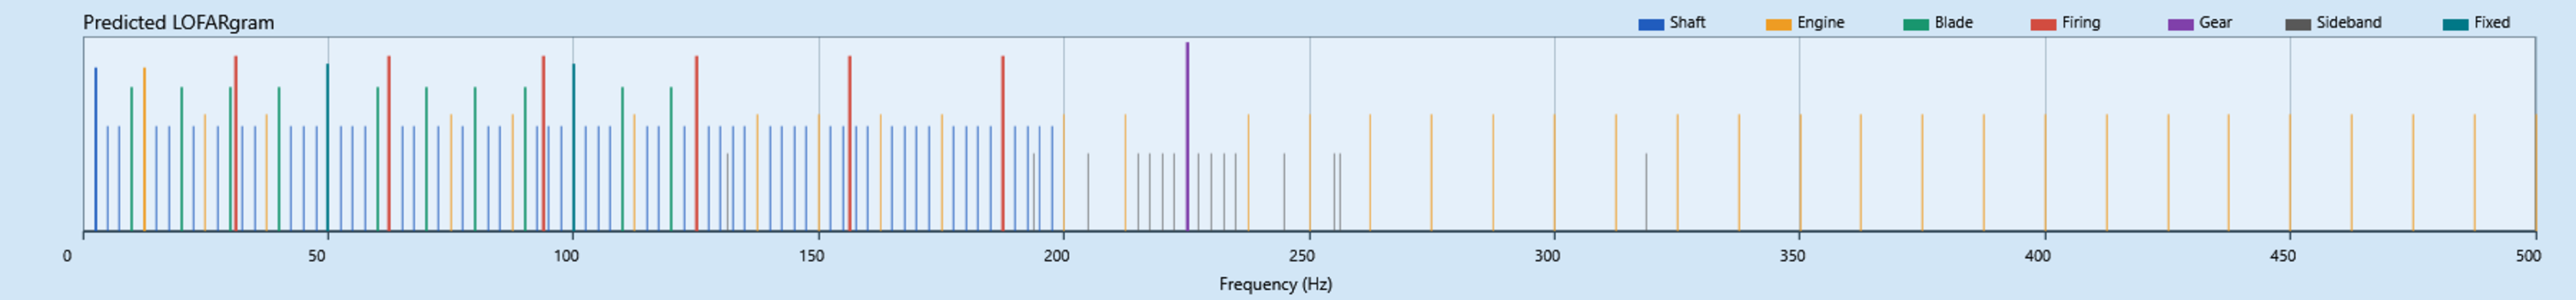
\includegraphics[width=\textwidth]{../img/actuals/lofar.pdf}
	\caption{All our data as a LOFARgram}
\end{figure}

\subsection{Recomended Workflow Using MACS}

Below is a recommended sequence for classifying an unknown contact. It applies equally to live capture and recorded file playback. Simply start capture or press [play] on a recording before beginning.
\subsubsection{Step 1 Clean up the signal}
\begin{compactenum}
    \item If own-ship or ambient noise is masking the target, designate a clean background recording as the noise reference and load it.
    \item Enable normalisation if tonals are weak against the noise floor. Adjust Scale until tonals are visible without the display saturating.
    \item If using a recorded file, apply the bandpass filter to isolate the frequency band of interest.
\end{compactenum}

\newcounter{myenum}
\setcounter{myenum}{\value{enumi}}

\subsubsection{Step 2 Identify tonals}
\begin{compactenum}
\setcounter{enumi}{\value{myenum}}
    \item On the LOFARgram (Panel A), note prominent vertical tonal lines.
    \item Use the harmonic cursor to test candidate fundamentals, place it on a suspected fundamental. Check whether the harmonic lines fall on other visible tonals. Do the same with sidebands.
    \item Zoom Fmin / Fmax to focus on dense tonal clusters.
    \item Mark confirmed tonals by selecting cursor mode and left-clicking on each line; right-click to clear.
\end{compactenum}

\setcounter{myenum}{\value{enumi}}

\subsubsection{Step 3 DEMON analysis}
\begin{compactenum}
\setcounter{enumi}{\value{myenum}}
    \item Open DEMON in Panel B.
    \item Set DEMON to a band with strong broadband noise (e.g. 500 - 5000 Hz).
    \item Identify the shaft rate peak (and / or diesel firing rate). Use the harmonic cursor to confirm the series.
    \item Note the shaft rate (SR) in rev/s.
\end{compactenum}

\setcounter{myenum}{\value{enumi}}

\subsubsection{Step 4 Cepstrum / ACF confirmation}
\begin{compactenum}
\setcounter{enumi}{\value{myenum}}  
    \item Switch Panel B to Cepstrum. Look for a quefrency peak confirming tonal spacing or shaft periodicity.
    \item Cross-check with ACF if needed.
\end{compactenum}

\setcounter{myenum}{\value{enumi}}

\subsubsection{Step 5 Record in database}
\begin{compactenum}
\setcounter{enumi}{\value{myenum}}
    \item In the right sidebar, enter a contact name in the \textbf{New Contact} field and click + Create with marked frequencies.
    \item Double-click the new contact to open the detail window.
    \item Enter propulsion type, blade count, shaft rate, speed, and any other known parameters. The app will auto-compute reduction factor and TPK.
    \item Add a note with the relevant recording filename for future reference (recording-to-contact linking is not yet available directly in the UI).
    \item \textbf{Save \& Close}
\end{compactenum}
\pagebreak
\section{Classification Examples and Exercises}
\textcolor{commentGreen}{*** WIP ***}

\subsection{Illustrated Example 1: A surface contact has been detected can you narrow down its class or type?}
\large Difficulty Rating \includegraphics{../img/actuals/Stars/"1 Star.jpg"}

\subsubsection{MNW In Game Tools}

A surface contact has been identified on broadband. Trackers are assigned for the LAB, WAA and the TB34 “Fatline” towed array. Listening to the sound from the LAB you hear:

\begin{compactenum}
    \item A distinct fast “swooshing” sound which you think maybe cavitation noise
    \item A faster underlying “tchouc tchouc tchouc” sound which you think is propellor blade noise
    \item You do not hear sounds characteristic of a diesel engine
    \item You do hear a prominent high pitch whine which sounds like a turbine or a high speed gear mesh
\end{compactenum}


Your initial conclusion is that this is a modern turbine powered ship cruising at a medium speed (15 - 25 kts) and that it is probably a warship. You base your provisional conclusions on the following tables from your personal notebook and the knowledge that most civilian ships are not turbine driven.

Civilian

\begin{tabularx}{\linewidth}{l l l X}
    \toprule
    \textbf{Speed Category} & \textbf{Knots} & \textbf{km/h} & \textbf{Typical Examples}\\
    \midrule
    \rowcolor[gray]{.9}Slow & Under 12 kn & Under 22 km/h & Large tankers, heavily loaded bulk carriers \\
    Medium & 12 - 20 kn & 22 - 37 km/h & Most cargo ships, ferries, many merchant vessels \\
    \rowcolor[gray]{.9}Fast & 20 - 30 kn & 37 - 56 km/h  & Cruise ships, fast ferries, some naval vessels\\
    Very fast & 30+ kn & 56+ km/h & Destroyers, patrol boats, high-speed ferries\\
    \bottomrule
\end{tabularx}

Warship

\begin{tabularx}{\linewidth}{l l l X}
\toprule
\textbf{Speed Category} & \textbf{Knots} & \textbf{km/h} & \textbf{Typical Examples}\\
\midrule
\rowcolor[gray]{.9}Slow & Under 15 kn & Under 28 km/h & Economic cruising, patrol, or fuel-saving transit \\
Medium & 15 - 25 kn & 28 - 46 km/h & Normal operating speed for most missions \\
\rowcolor[gray]{.9}Fast & 25 - 35 kn & 46 - 65 km/h  & High-speed transit, tactical maneuvers\\
Very fast & 35+ kn & 65+ km/h & Fast attack craft, some hydrofoils, exceptional warships\\
\bottomrule
\end{tabularx}

Using the sound output feature of the sonar suite you find it is possible to count the more prominent “swooshing” sound. You do this over 60 seconds several times then take an average. By doing this you establish that there are an average of 130 beats per minute which is about 2.1 Hz (130 / 60). Unfortunately you can't do the same for the higher frequency blade rate as there is no facility to slow the sound down in game at this time.

Top Tip: Counting sounds like this can be made much easier by using a beat tap counter which will automatically give you the count / beats per minute. Some will even listen to the sound and give you a count. There are several available free for iPad / iPhone and Android

In MNW you switch to narrowband and attach the TB34. You start at a wide window of frequencies (0 - 3600 Hz) which produces the following display (Figure 16).

You immediately recognise a fairly strong tonal at 3 kHz (3000 Hz) which you think is the high pitched whine which you attribute to the turbine or possibly the reduction gear. You also spot a strong diffuse band centred around 261 HZ (150 - 400 Hz) and another less prominent band between 1050 and 1350 Hz.

At this scale it is not possible to see any other tonals so you select a drilled in view (Figure 17). At this frequency range it is possible to see another faint tonal around 33 Hz. This is quite difficult to spot and requires high input and gain settings which washes out most of the screen so details within the broader noise bands are lost. At this stage you do not know what is causing the 33 Hz tonal so you carefully note it before moving on to a DEMON analysis in an effort to gain some insight into the ship’s speed.

DEMON can provide information about the shaft rate (SR) and the blade count (BC). Sometimes it is possible to identify the number of propeller shafts (Figure 18). Our system shows a strong tonal at 2.2 Hz (Note in the picture the cursor is offset) which is hypothesised to be the shaft fundamental.

\begin{figure}[ht]
	\centering
	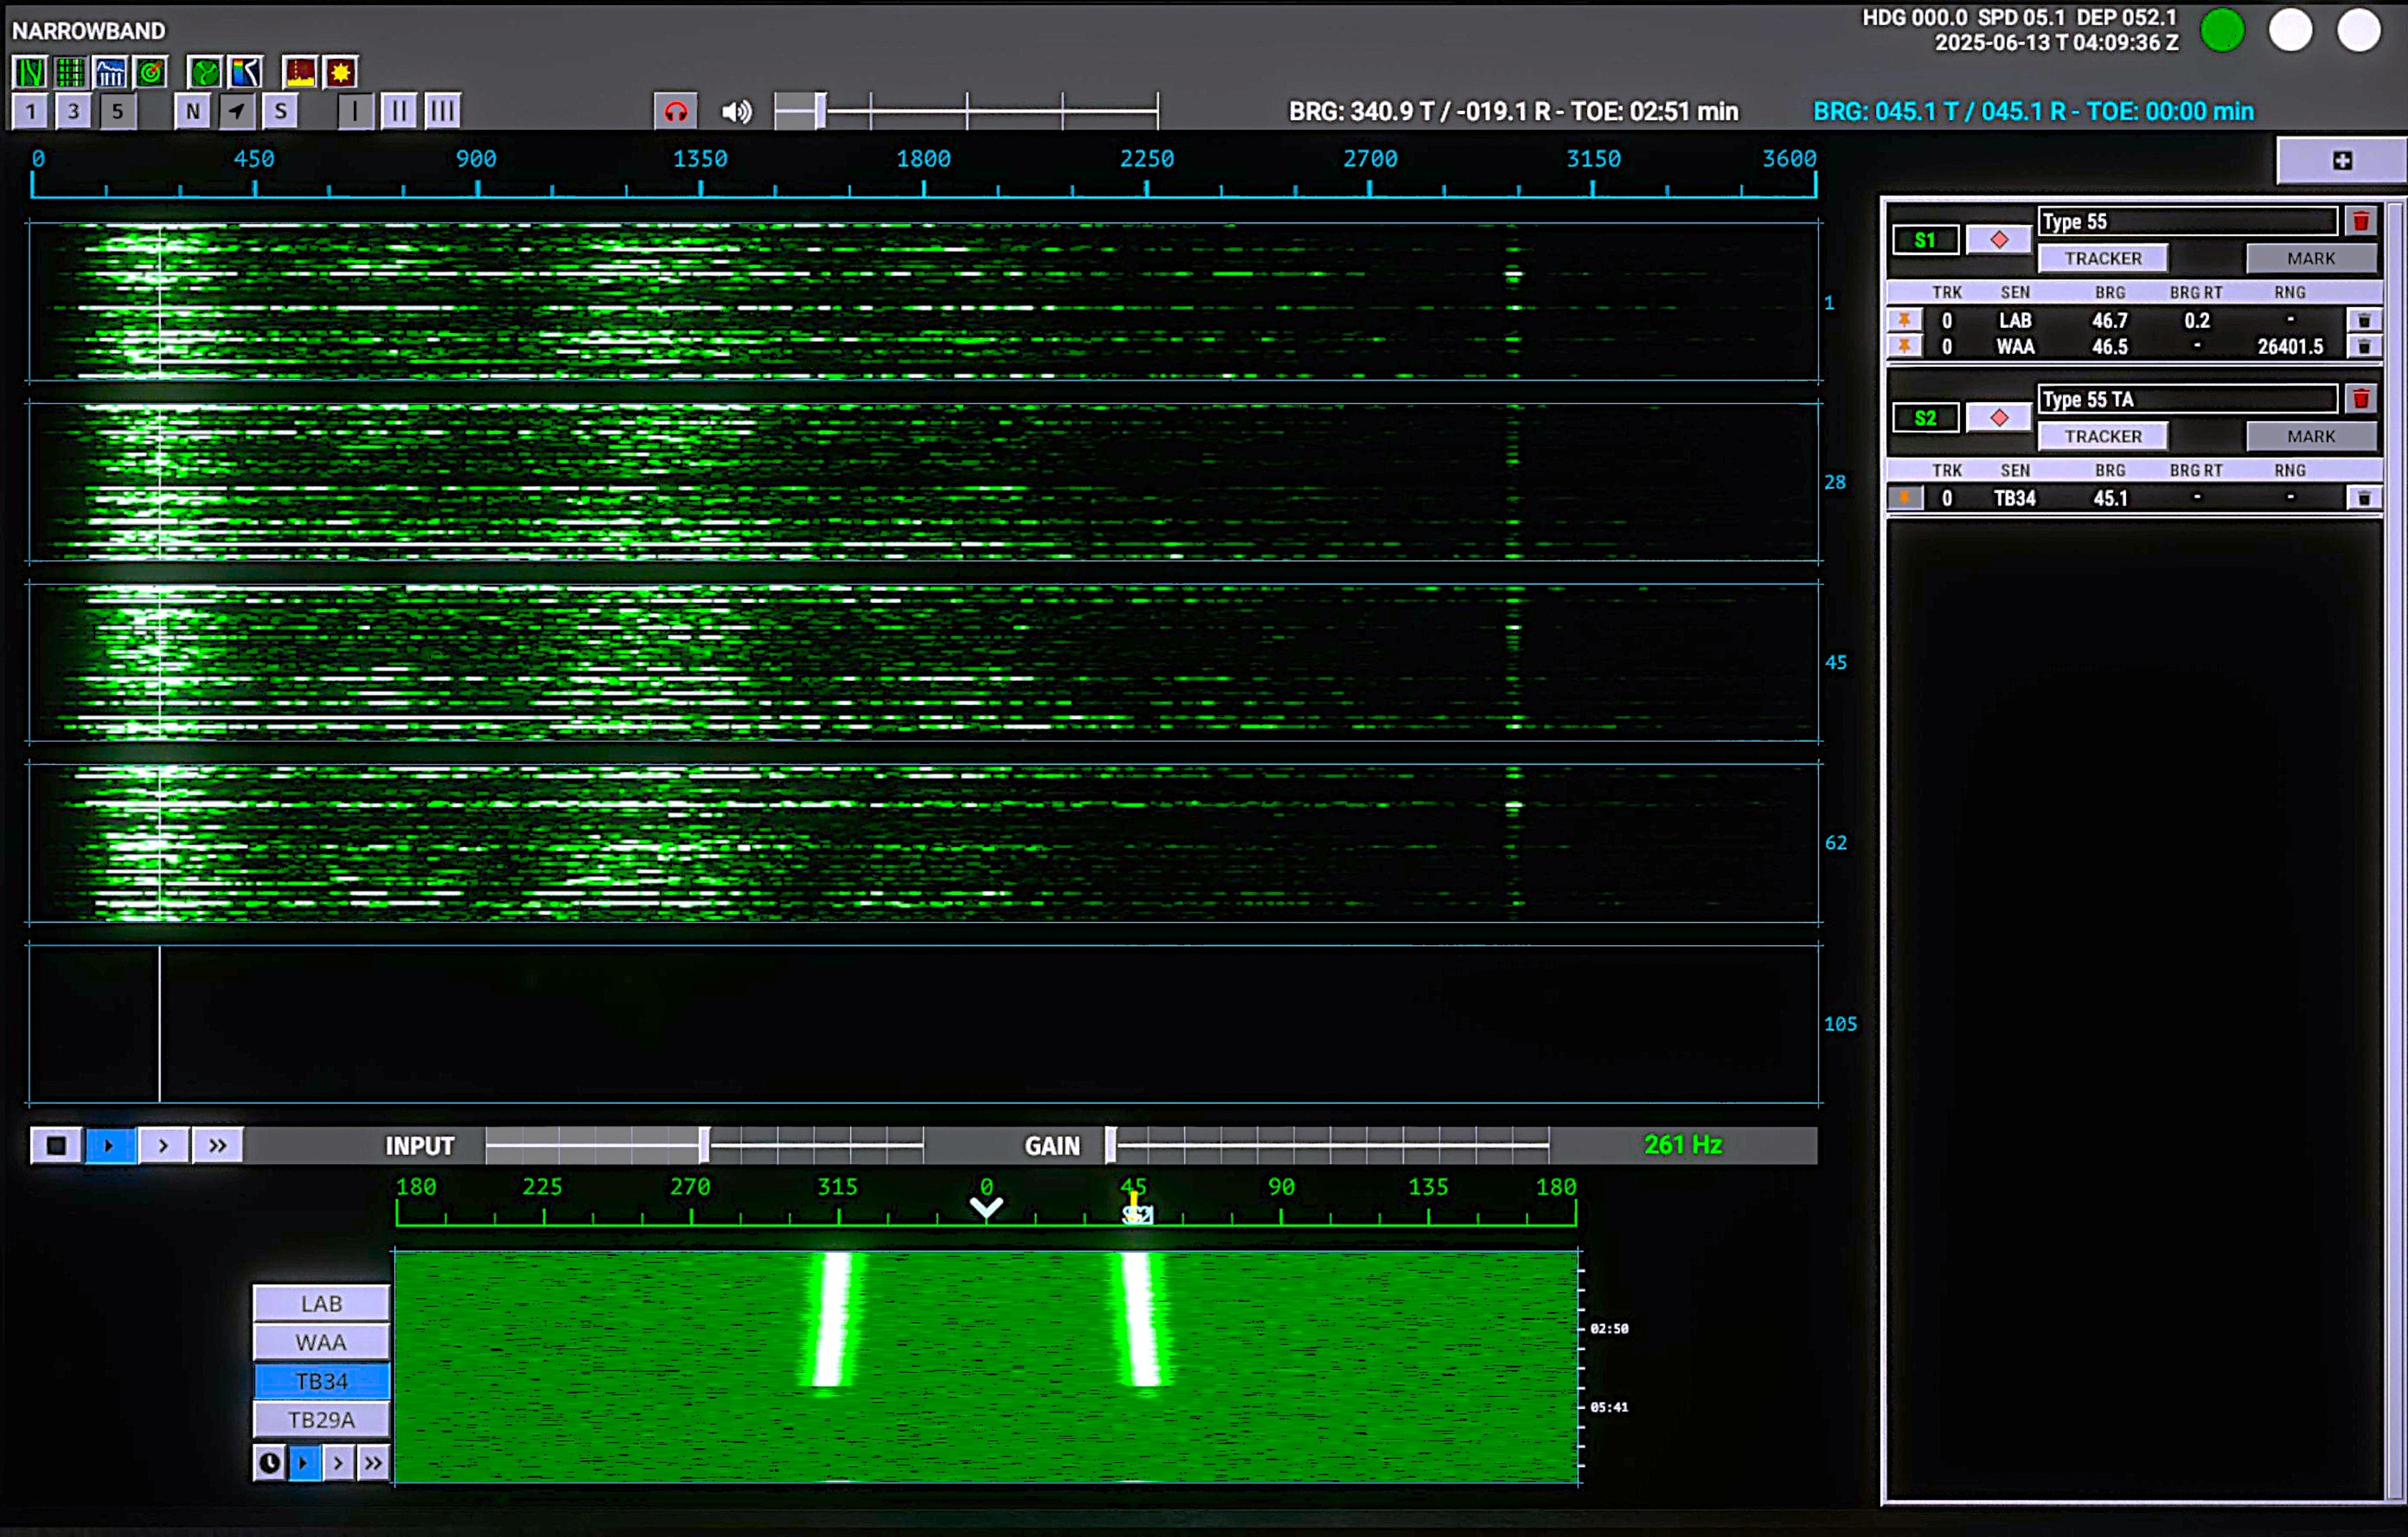
\includegraphics[width=310px]{../img/actuals/Type55_01a.pdf}
	\caption{Narrowband 0 - 3600 Hz}
\end{figure}

\begin{figure}[ht]
	\centering
	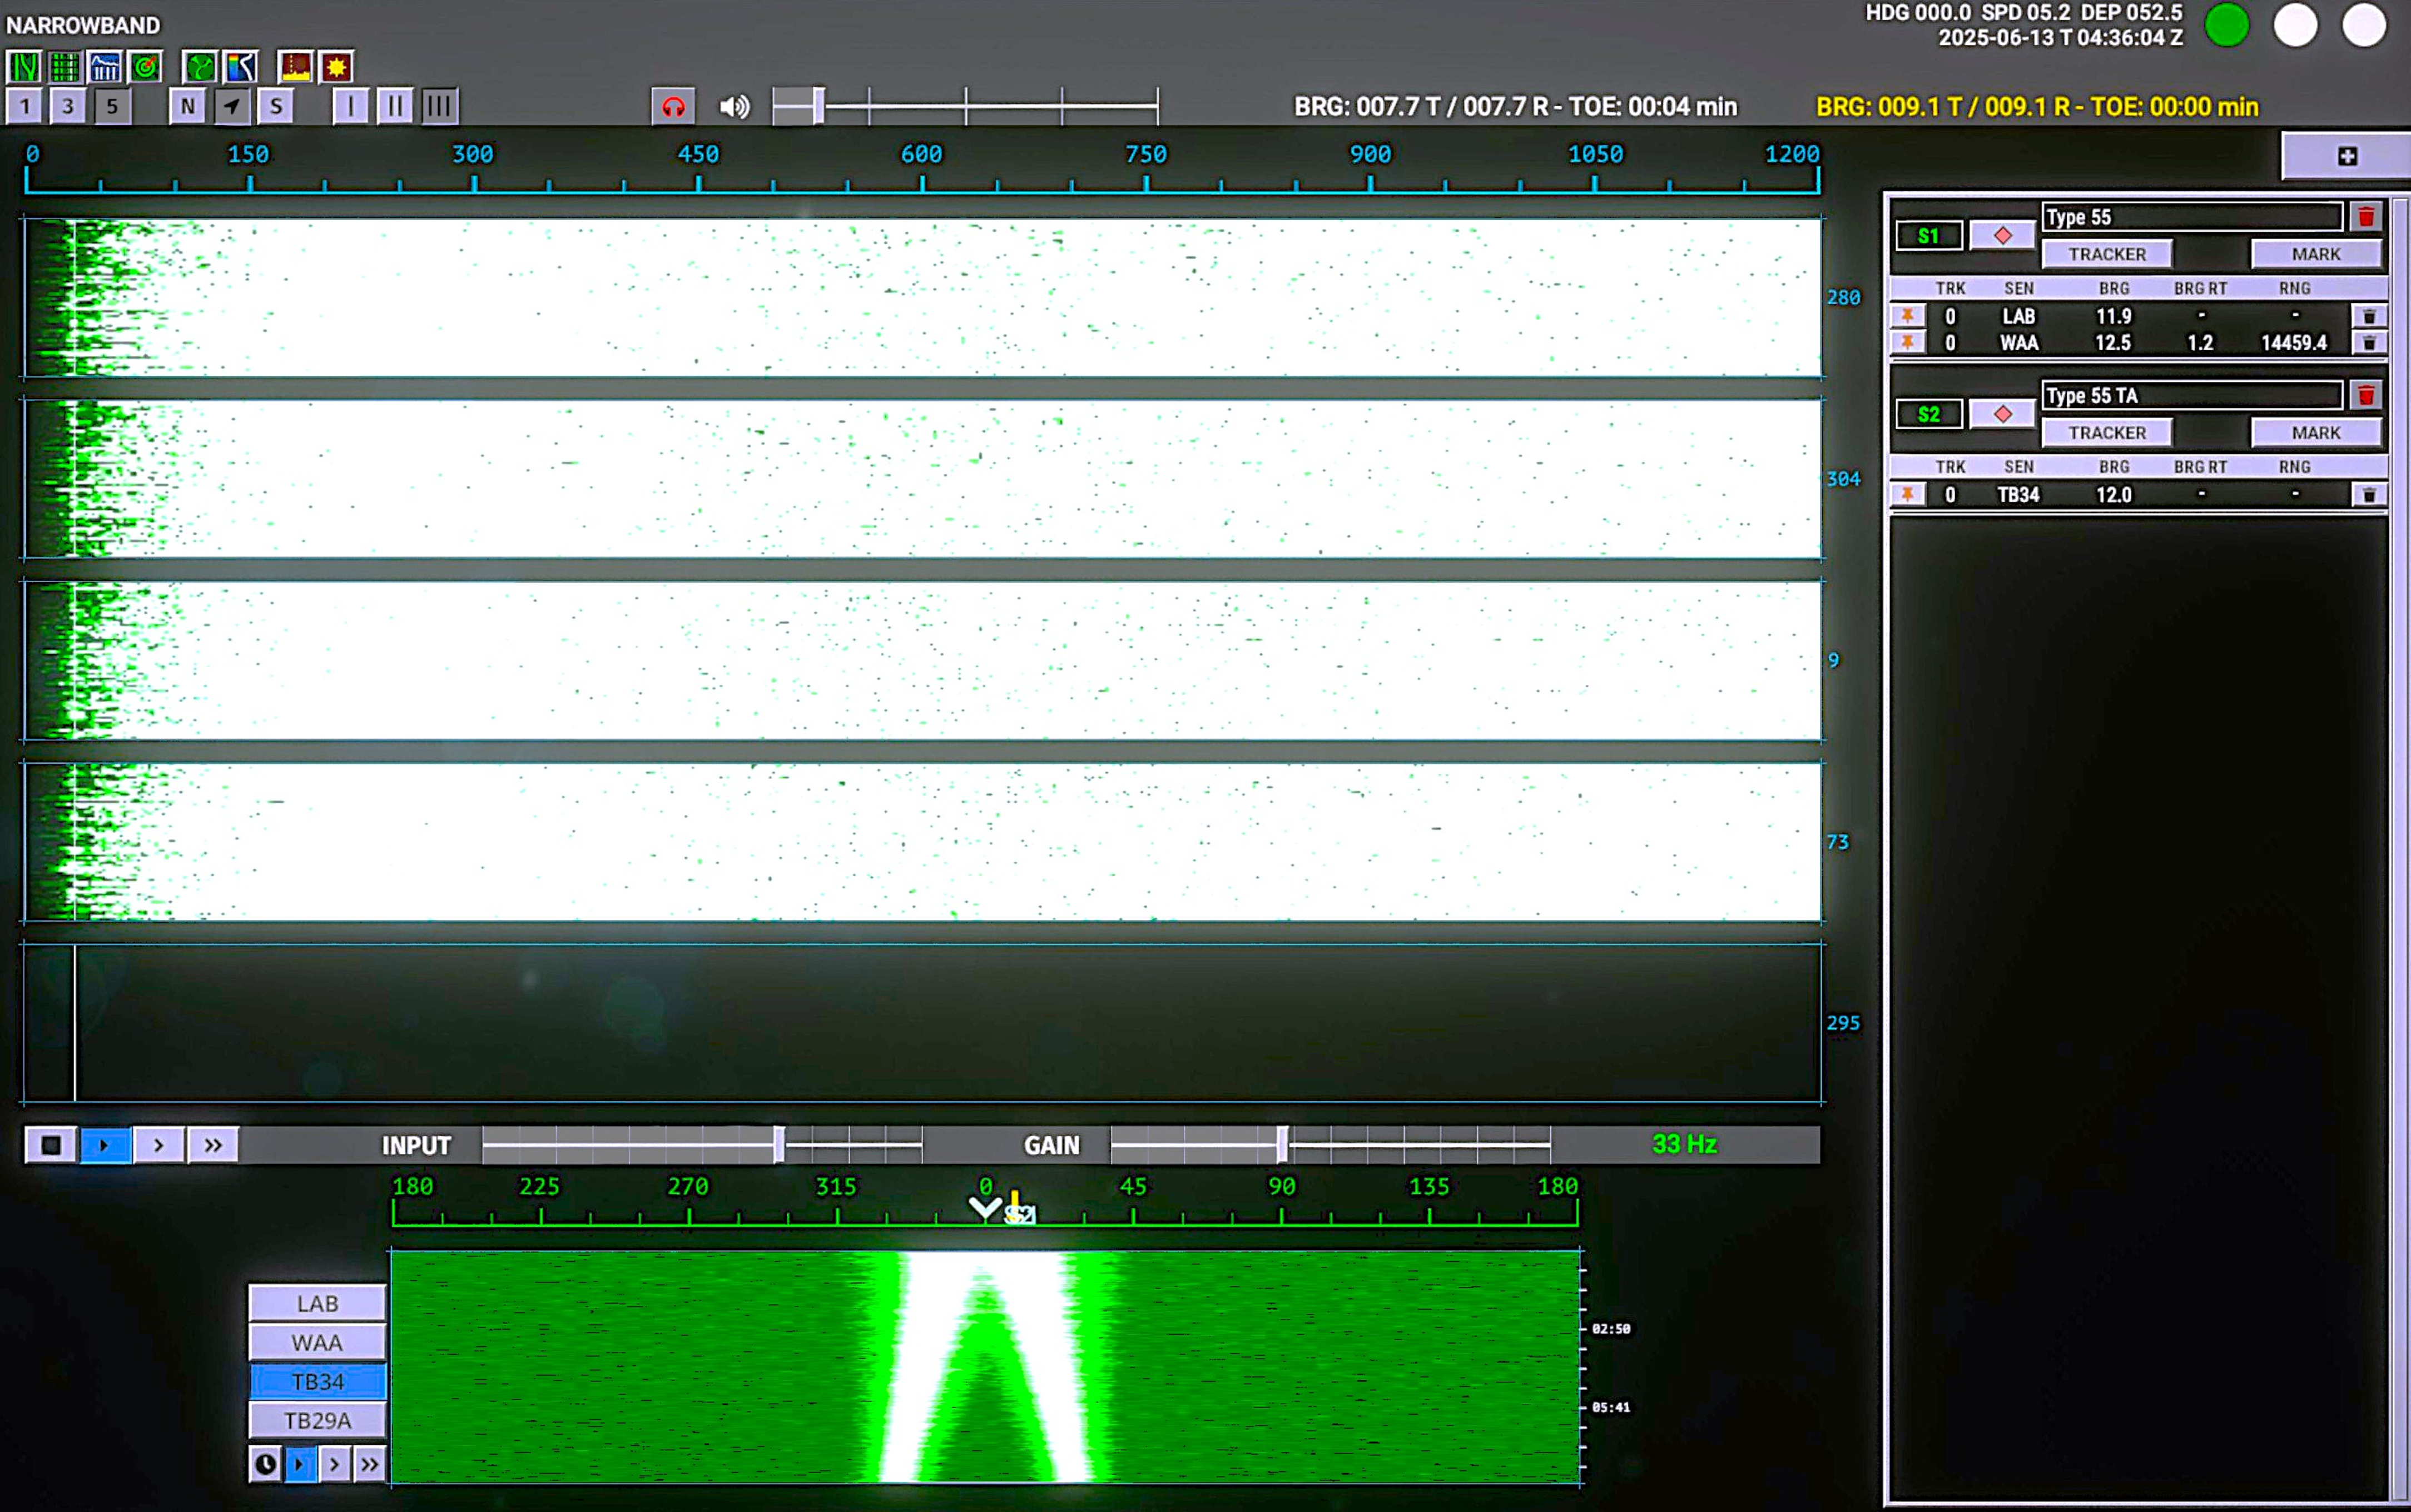
\includegraphics[width=310px]{../img/actuals/Type55_01b.pdf}
	\caption{Narrowband 0 - 1200 Hz - a faint 33Hz tonal}
\end{figure}

\begin{figure}[H]
	\centering
	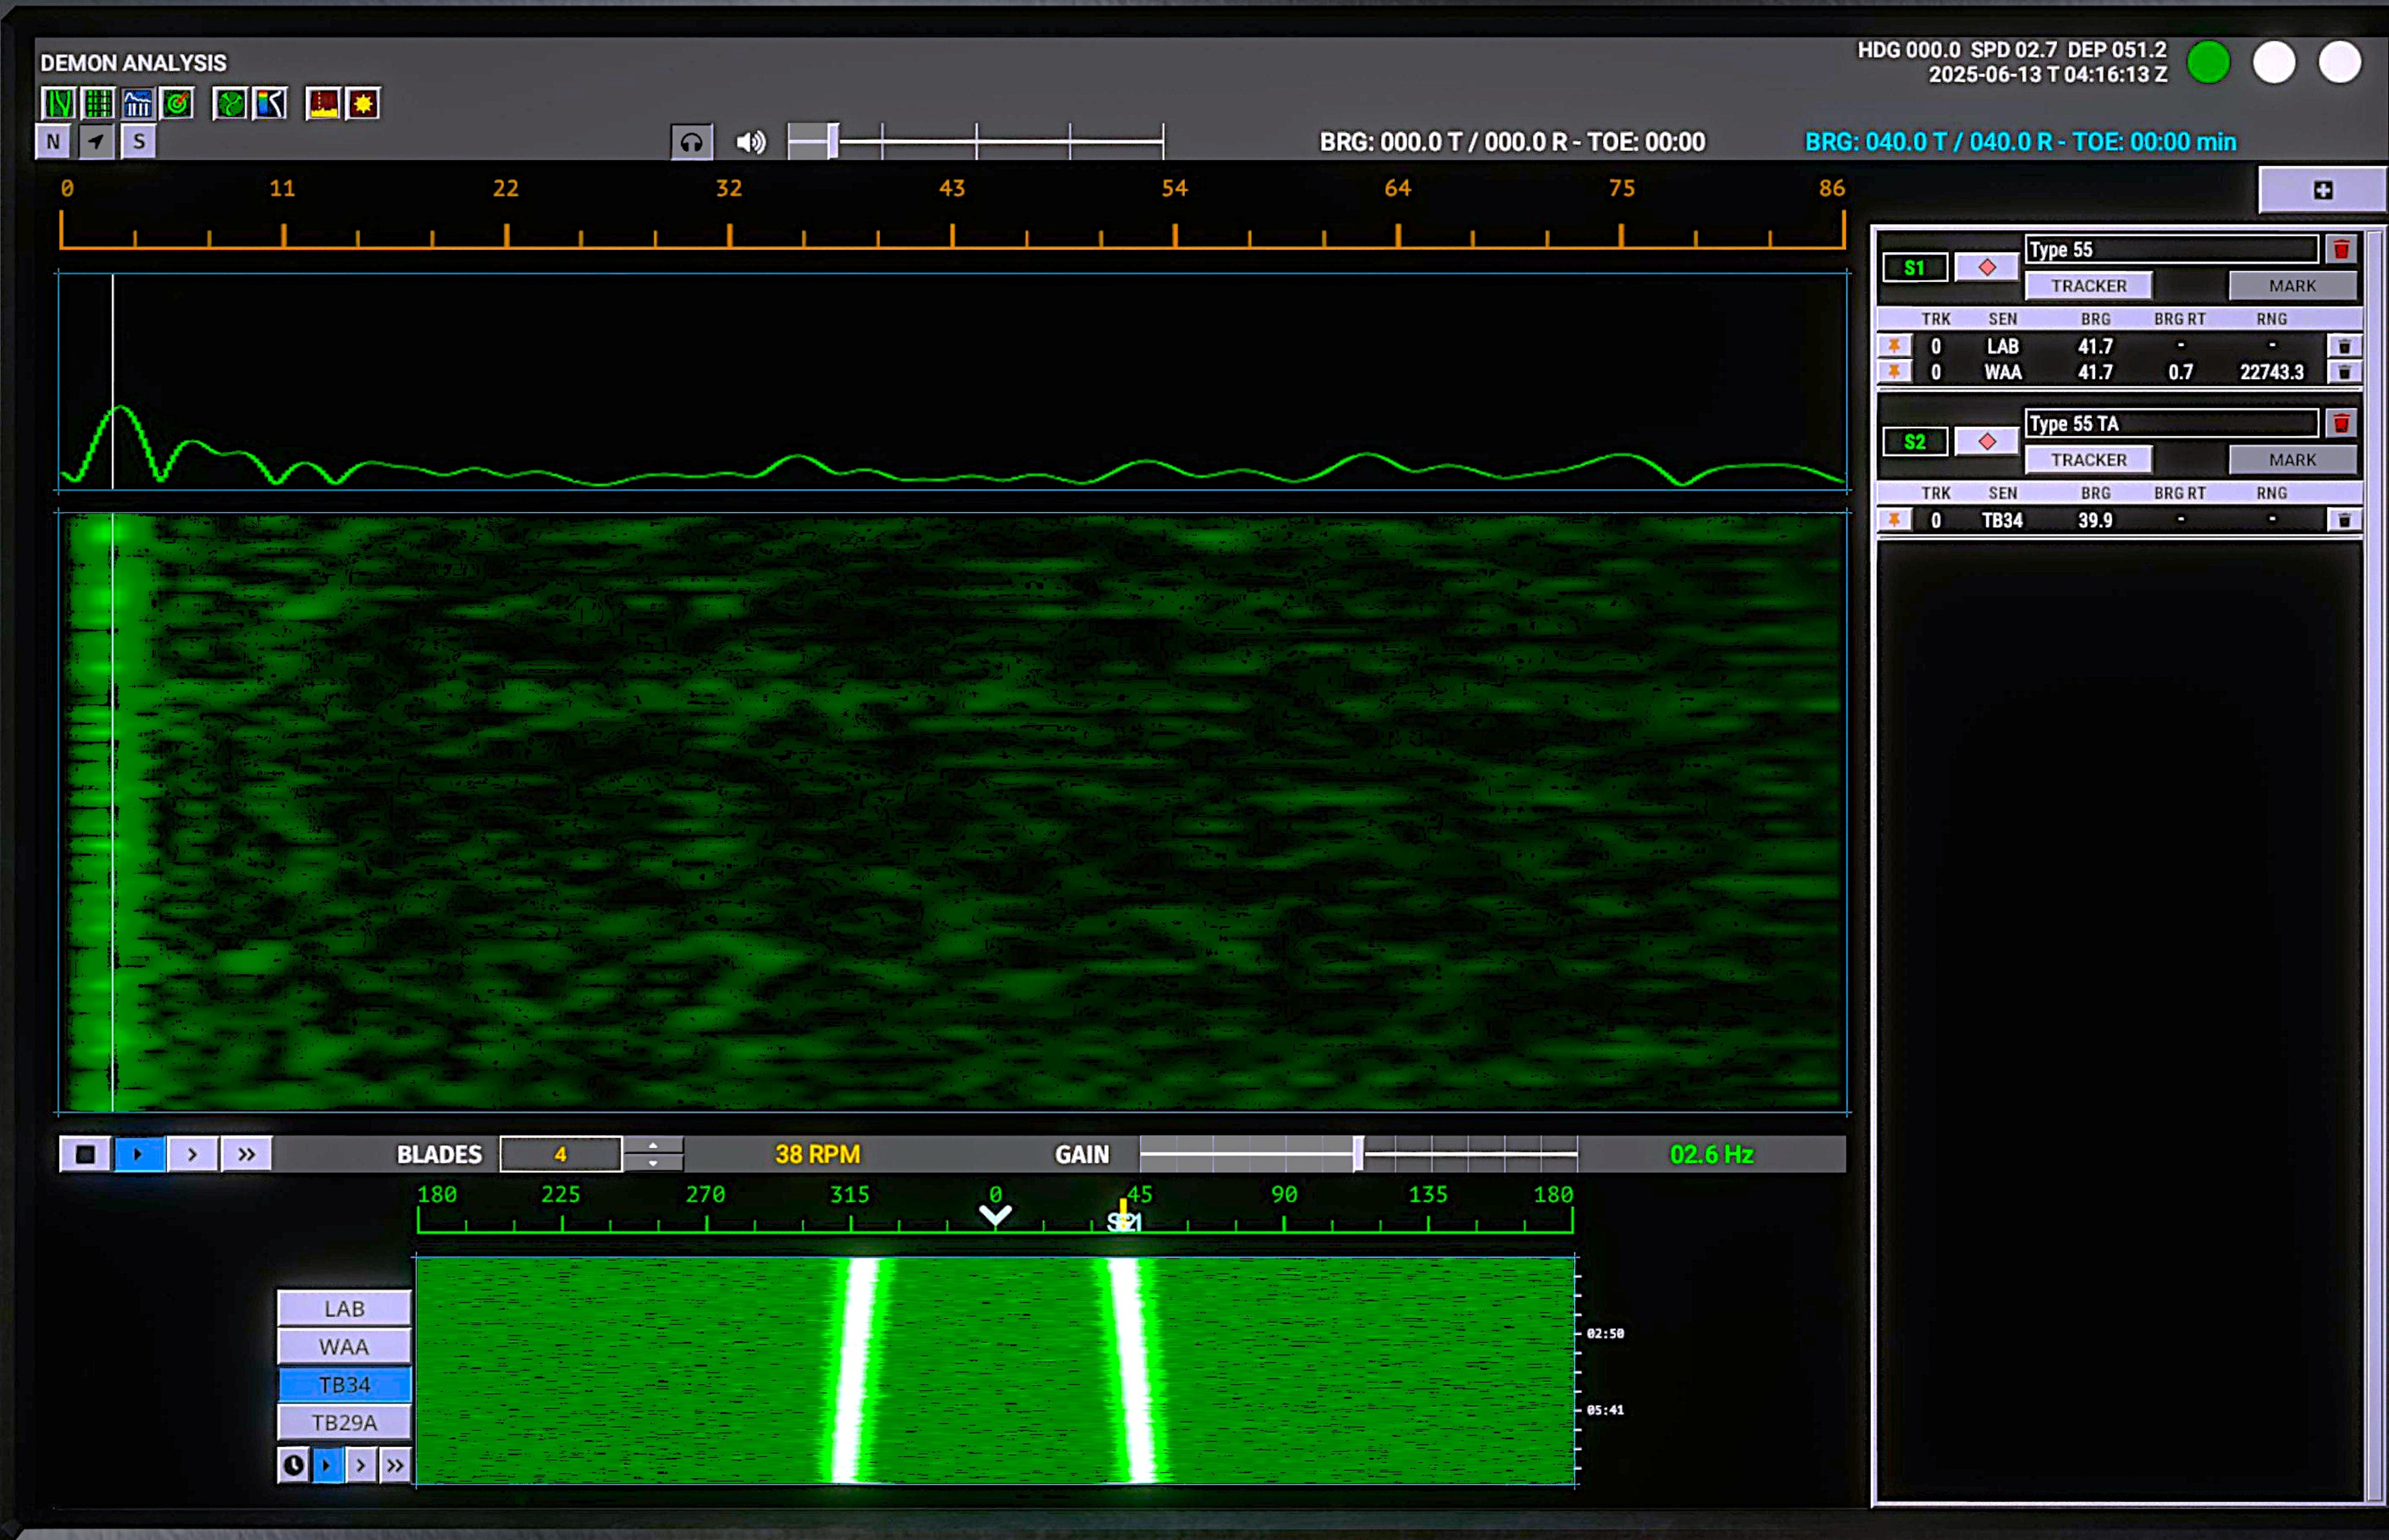
\includegraphics[width=310px]{../img/actuals/Type55_02.pdf}
	\caption{DEMON Display}
\end{figure}

It is difficult to get the exact frequency because the tonal is quite smeared as if there were two lines on top of each other slightly offset. If that were the case it would suggest this vessel has at least two shafts. The rotation frequency of 2.2 Hz gives a shaft rotation speed of 132 RPM ($2.2 \times 60$).

The DEMON waterfall is not providing any clear indication of the number of propeller blades, however the smooth line plot above does show some slight indication of blades. Including the shaft it is just possible to suggest 5 humps and then a series of what could be harmonics further up. This could be indicative of a five bladed propeller which, if this is true would give a blade rate of 11 Hz ($5 \times 2.2$) or 660 RPM ($11 \times 60$). However, the data is speculative and definitely requires a more detailed analysis.

\subsubsection{MACS Tools}

In order to improve your analysis and refine your hypothesis you decide to utilise the advanced tools available in MACS.

Your first step is to capture a recording of the sound of the contact. How to do this depends on your PC sound configuration but most often this will be a simple loopback arrangement (See Section 3). Capture a recording by clicking the record button on the top toolbar. The recording should be long enough to capture any periodic variation in the sound, 2 minutes should be plenty although longer recordings may be necessary if you are monitoring changes of speed or direction. As soon as you stop the recording it will appear in the recordings panel on the lower right of the application. It is highly recommended that you change the generated name to one that is more user friendly. Do this by double clicking the recording and renaming it. Once you have your recording you can analyse the sound in a more structured way without having to deal with real time issues.

As for the in game tools your first review should be using your ears and your experience. We can tell from the recording that:

\begin{compactenum}
    \item No diesel firing.
    \item Distinct slower “swooshing” sound.
    \item Underlying faster “blade” sound.
    \item High pitched whine at 3 kHz possibly turbine or gear mesh.
\end{compactenum}


You first focus on the 3 kHz tonal which you believe is responsible for the high pitched whine which you suggest is either the turbine or the reduction gear mesh frequency. By setting the bandpass frequency to 0 - 2500Hz the sound is eliminated from the playback strengthening the hypothesis.

Next assess the distinctive audible regular “swooshing” sound and the faster chopping sound. Using a beat counter the louder sound is found to be 134 BPM. You propose that the sound is made by cavitation and can be used to estimate the shaft RPM. 134 RPM is 2.2 Hz. When we come to look at the LOFARgram we will look out for the shaft fundamental at that value.

Counting the Blade Rate is more difficult because it is too fast. Using MACS we have the option to slow the playback, a feature MNW does not have at this point. Slowing the playback speed to 0.25 it is possible to count each blade passing. For this exercise several counts over 30 seconds were conducted and then averaged.

Blade RPM playback at 0.25 speed over 30s averaged: $82 \times 2 \times 4$ ( $\times 2$ because 30s $\rightarrow$ 1 minute and $\times 4$ because 0.25 speed) = 656 RPM or 11 Hz

Blades: $654 \div 134 = 4.9$ (5 Blades) It is always likely that the numbers will not be exact as the sound path from source to receiver is never as straight forward as theory would suggest. Propellers can be out of balance and modulate shaft and blade sounds. Gears and bearings wear unevenly. Ships can change speed and direction introducing doppler effects which can distort or enhance frequencies. Bear in mind these “confounders”, you should expect measures never to be exact. You will use your experience to judge whether 4.9 should be 5 when 4.69 is too many deviations to be reliable.

\begin{faintquote}
    Top Tip: Take notes continuously they will become a powerful tool to help you be more effective and efficient at narrowing down target classification
\end{faintquote}

\begin{faintquote}
    It should be clear by now that the process is one of hypothesis forming, testing and falsification. Ultimately you are never going to be 100\% confident in your analysis it is always going to be on the balance of probabilities. Becoming comfortable with working with uncertainty is key to being effective.
\end{faintquote}

\textbf{LOFAR}

Our next step is to look at MACS' equivalent of the MNW's narrowband and DEMON plus some additional tools that have yet to appear in game.

One of the many features of MACS is the ability to tune input and output parameters. This is, at the time of writing, quite limited in game. To get the best results you will need to tweak these parameters so you must understand what they do. Details are discussed in Sections 2 and 5 and Appendix B. Unfortunately it is not possible to give hard and fast guidance as everyone's screens will vary in capability, refresh rates or resolution. For Figure 19 the following settings were used.

\begin{compactenum}
    \item Fmin = 0 Fmax = 5000
    \item Floor = -90 Dyn = 55
    \item Norm = Off
    \item FFT Overlap = Off
    \item FFT = 131072
\end{compactenum}

Note: This level of detail is very slow to plot however this is realistic. It is possible to speed things up by reducing the FFT or increasing the overlap setting at the cost of reducing detail.

\begin{figure}[ht]
	\centering
	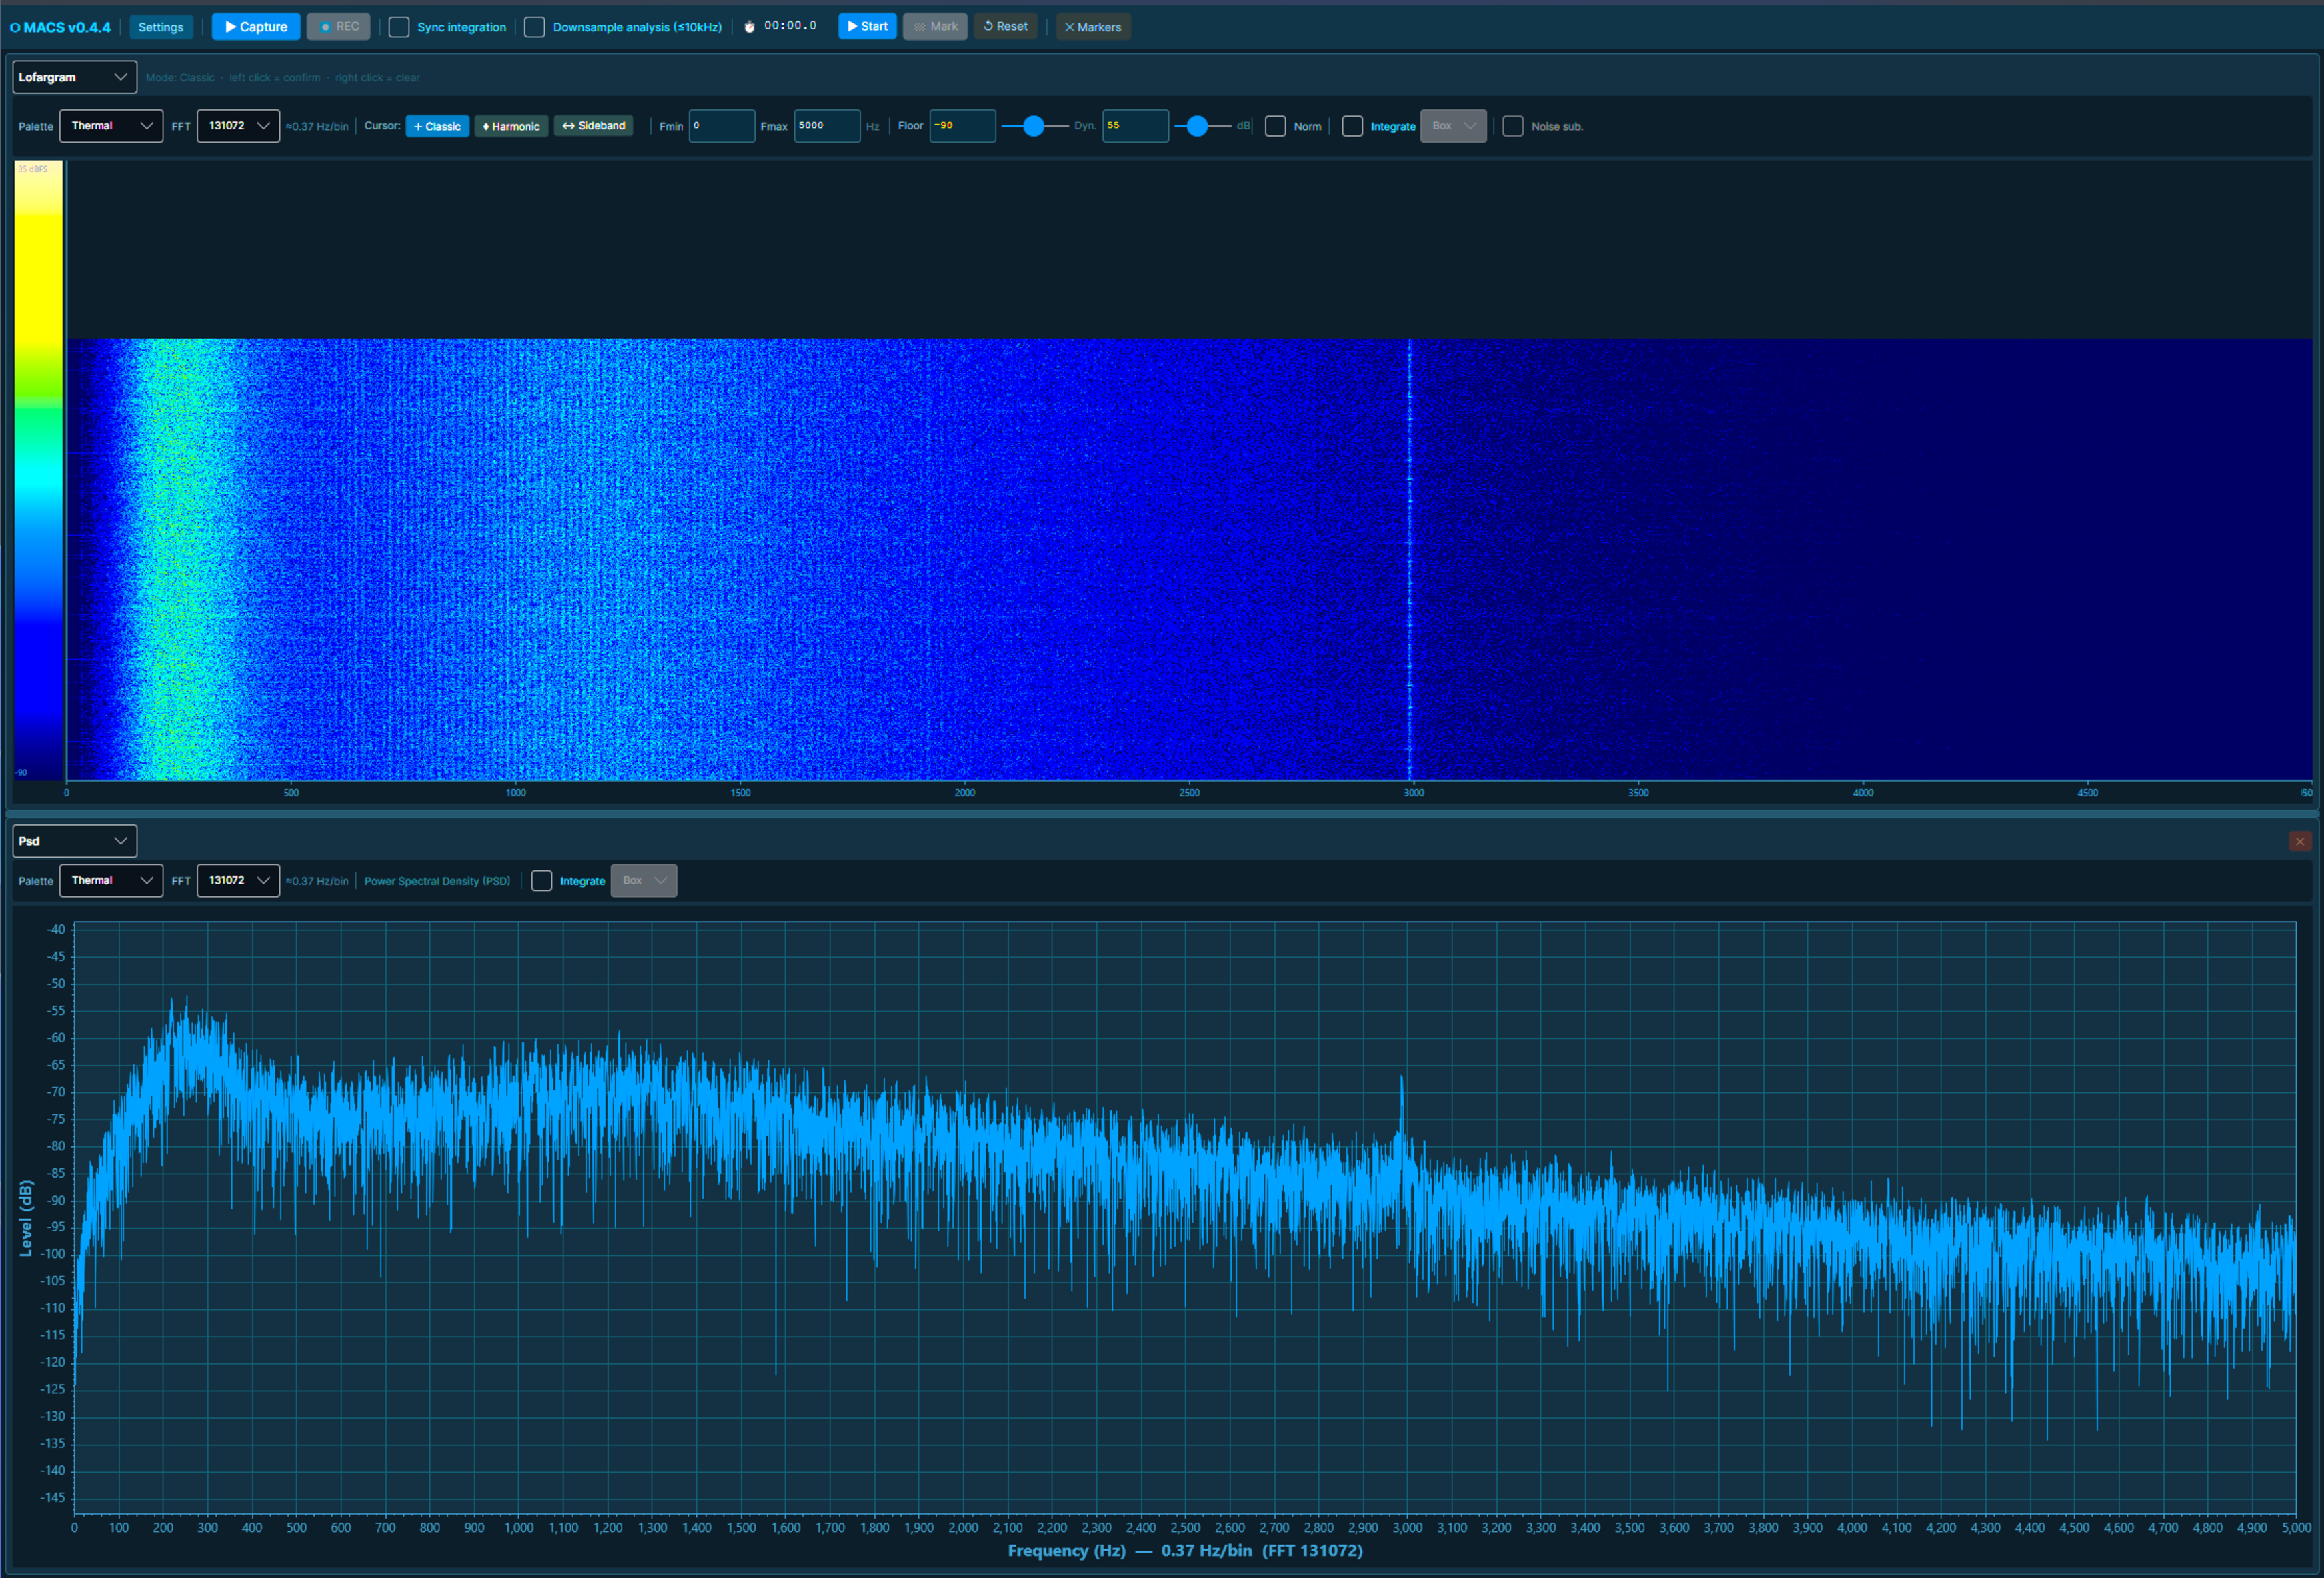
\includegraphics[width=300px]{../img/actuals/Type55_03.pdf}
	\caption{LOFARgram Fmin = 0 Hz - Fmax = 5000 Hz}
\end{figure}

The LOFARgram whilst much more detailed should be familiar. It shows and confirms our findings from the in game tools.

\begin{compactenum}
    \item Initial MNW narrowband screen shows a broad spectrum of noise between 150 Hz and 400 Hz.
    \item Another fainter band between 1050 Hz and 1350 Hz
    \item A high pitched whine / whistle at 3 kHz
    \item Narrow band does not have the distinctive lines associated with diesel firing
\end{compactenum}

\begin{figure}[ht]
	\centering
	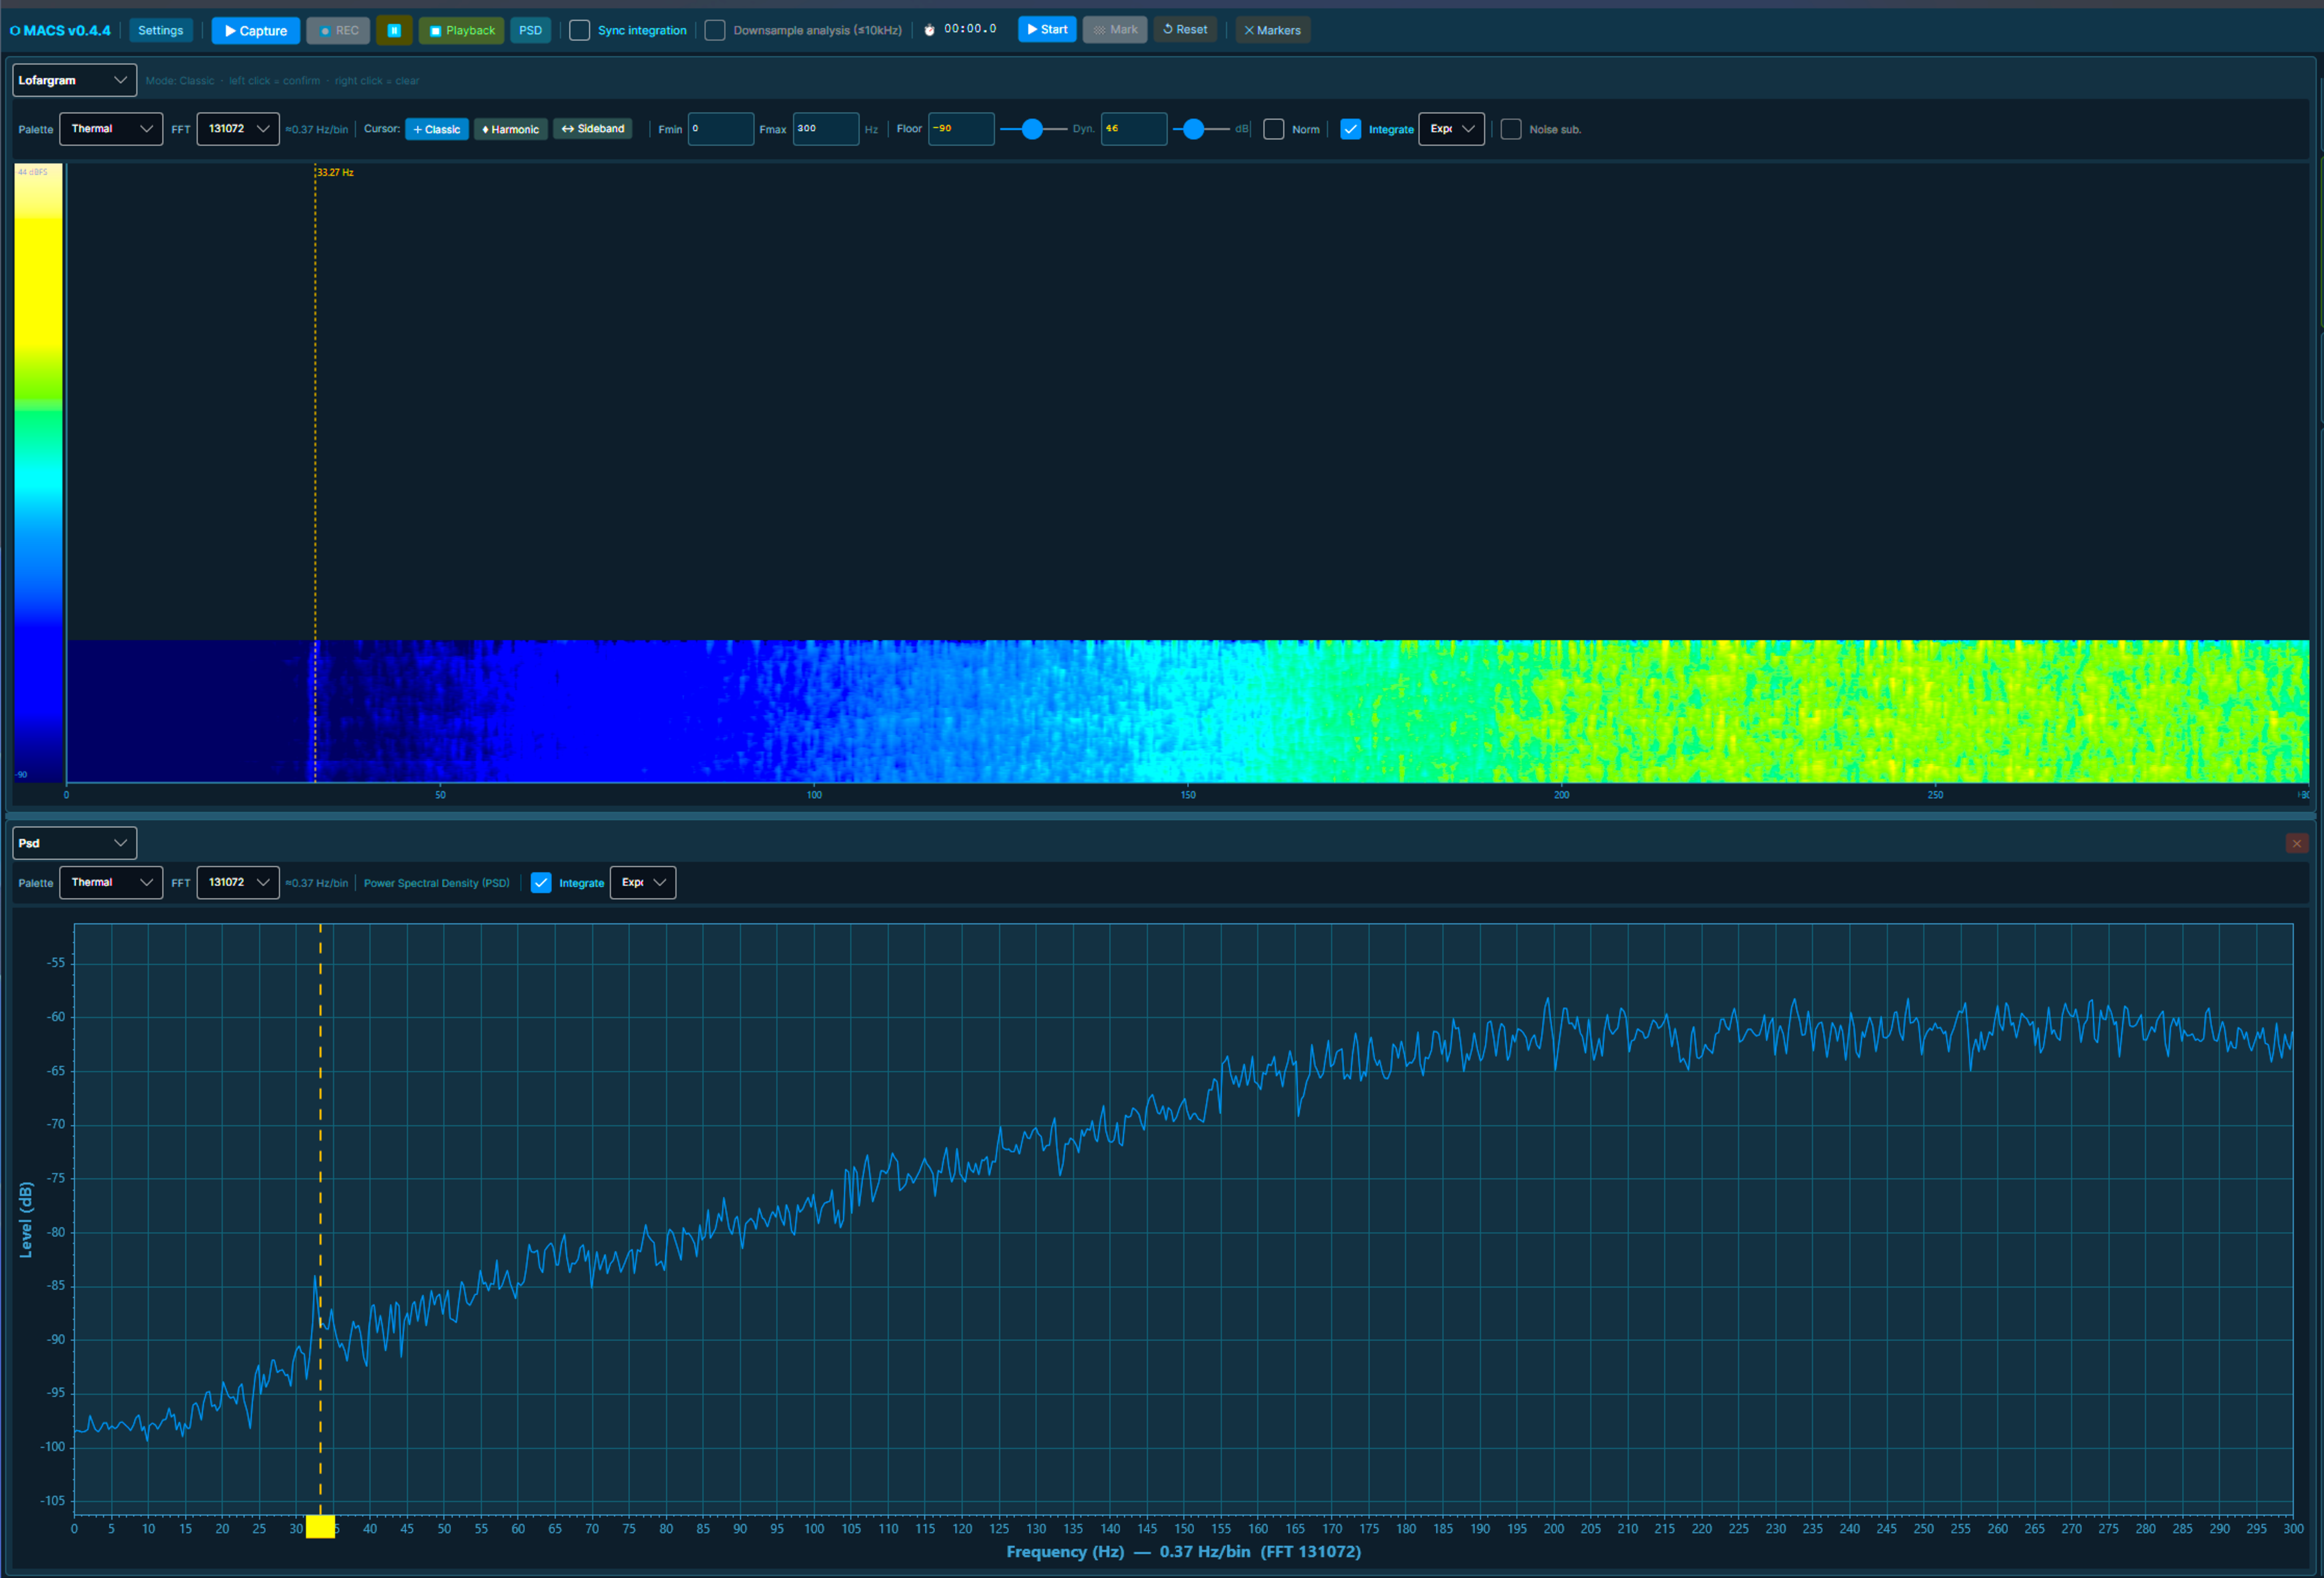
\includegraphics[width=300px]{../img/actuals/Type55_04.pdf}
	\caption{LOFARgram Fmin = 0 Hz - Fmax = 500 Hz}
\end{figure}

We repeat the plot but this time we reduce the Fmax parameter to 500 Hz because it would be useful to see if there are any fainter tonals that are crammed against the left hand side of the chart. Using the following settings we get Figure 20 revealing a hidden tonal which also confirms our earlier findings, the faint tonal seen in MNW is confirmed and narrowed down to 33.27 Hz

\begin{compactenum}
    \item Fmin = 0 Fmax = 500
    \item Floor = -90 Dyn 46
    \item Norm = Off
    \item FFT Overlap = Off
    \item FFT = 131072
    \item LOFARgram integration = Exp Box frame count = 16 Exponential time constant = 8 Fixed duration = 5
\end{compactenum}

The DEMON clearly shows a lone dual-sync tonal at 2.21 Hz Figure 21, which translates to 132.6 RPM closely matching audio SRPM. The line has a dual structure with a helical appearance which could possibly indicate a dual shaft.There is some indication of sidebands around the 2.21 Hz tonal which may indicate some modulation either by propellers or some other source.

\begin{figure}[H]
	\centering
	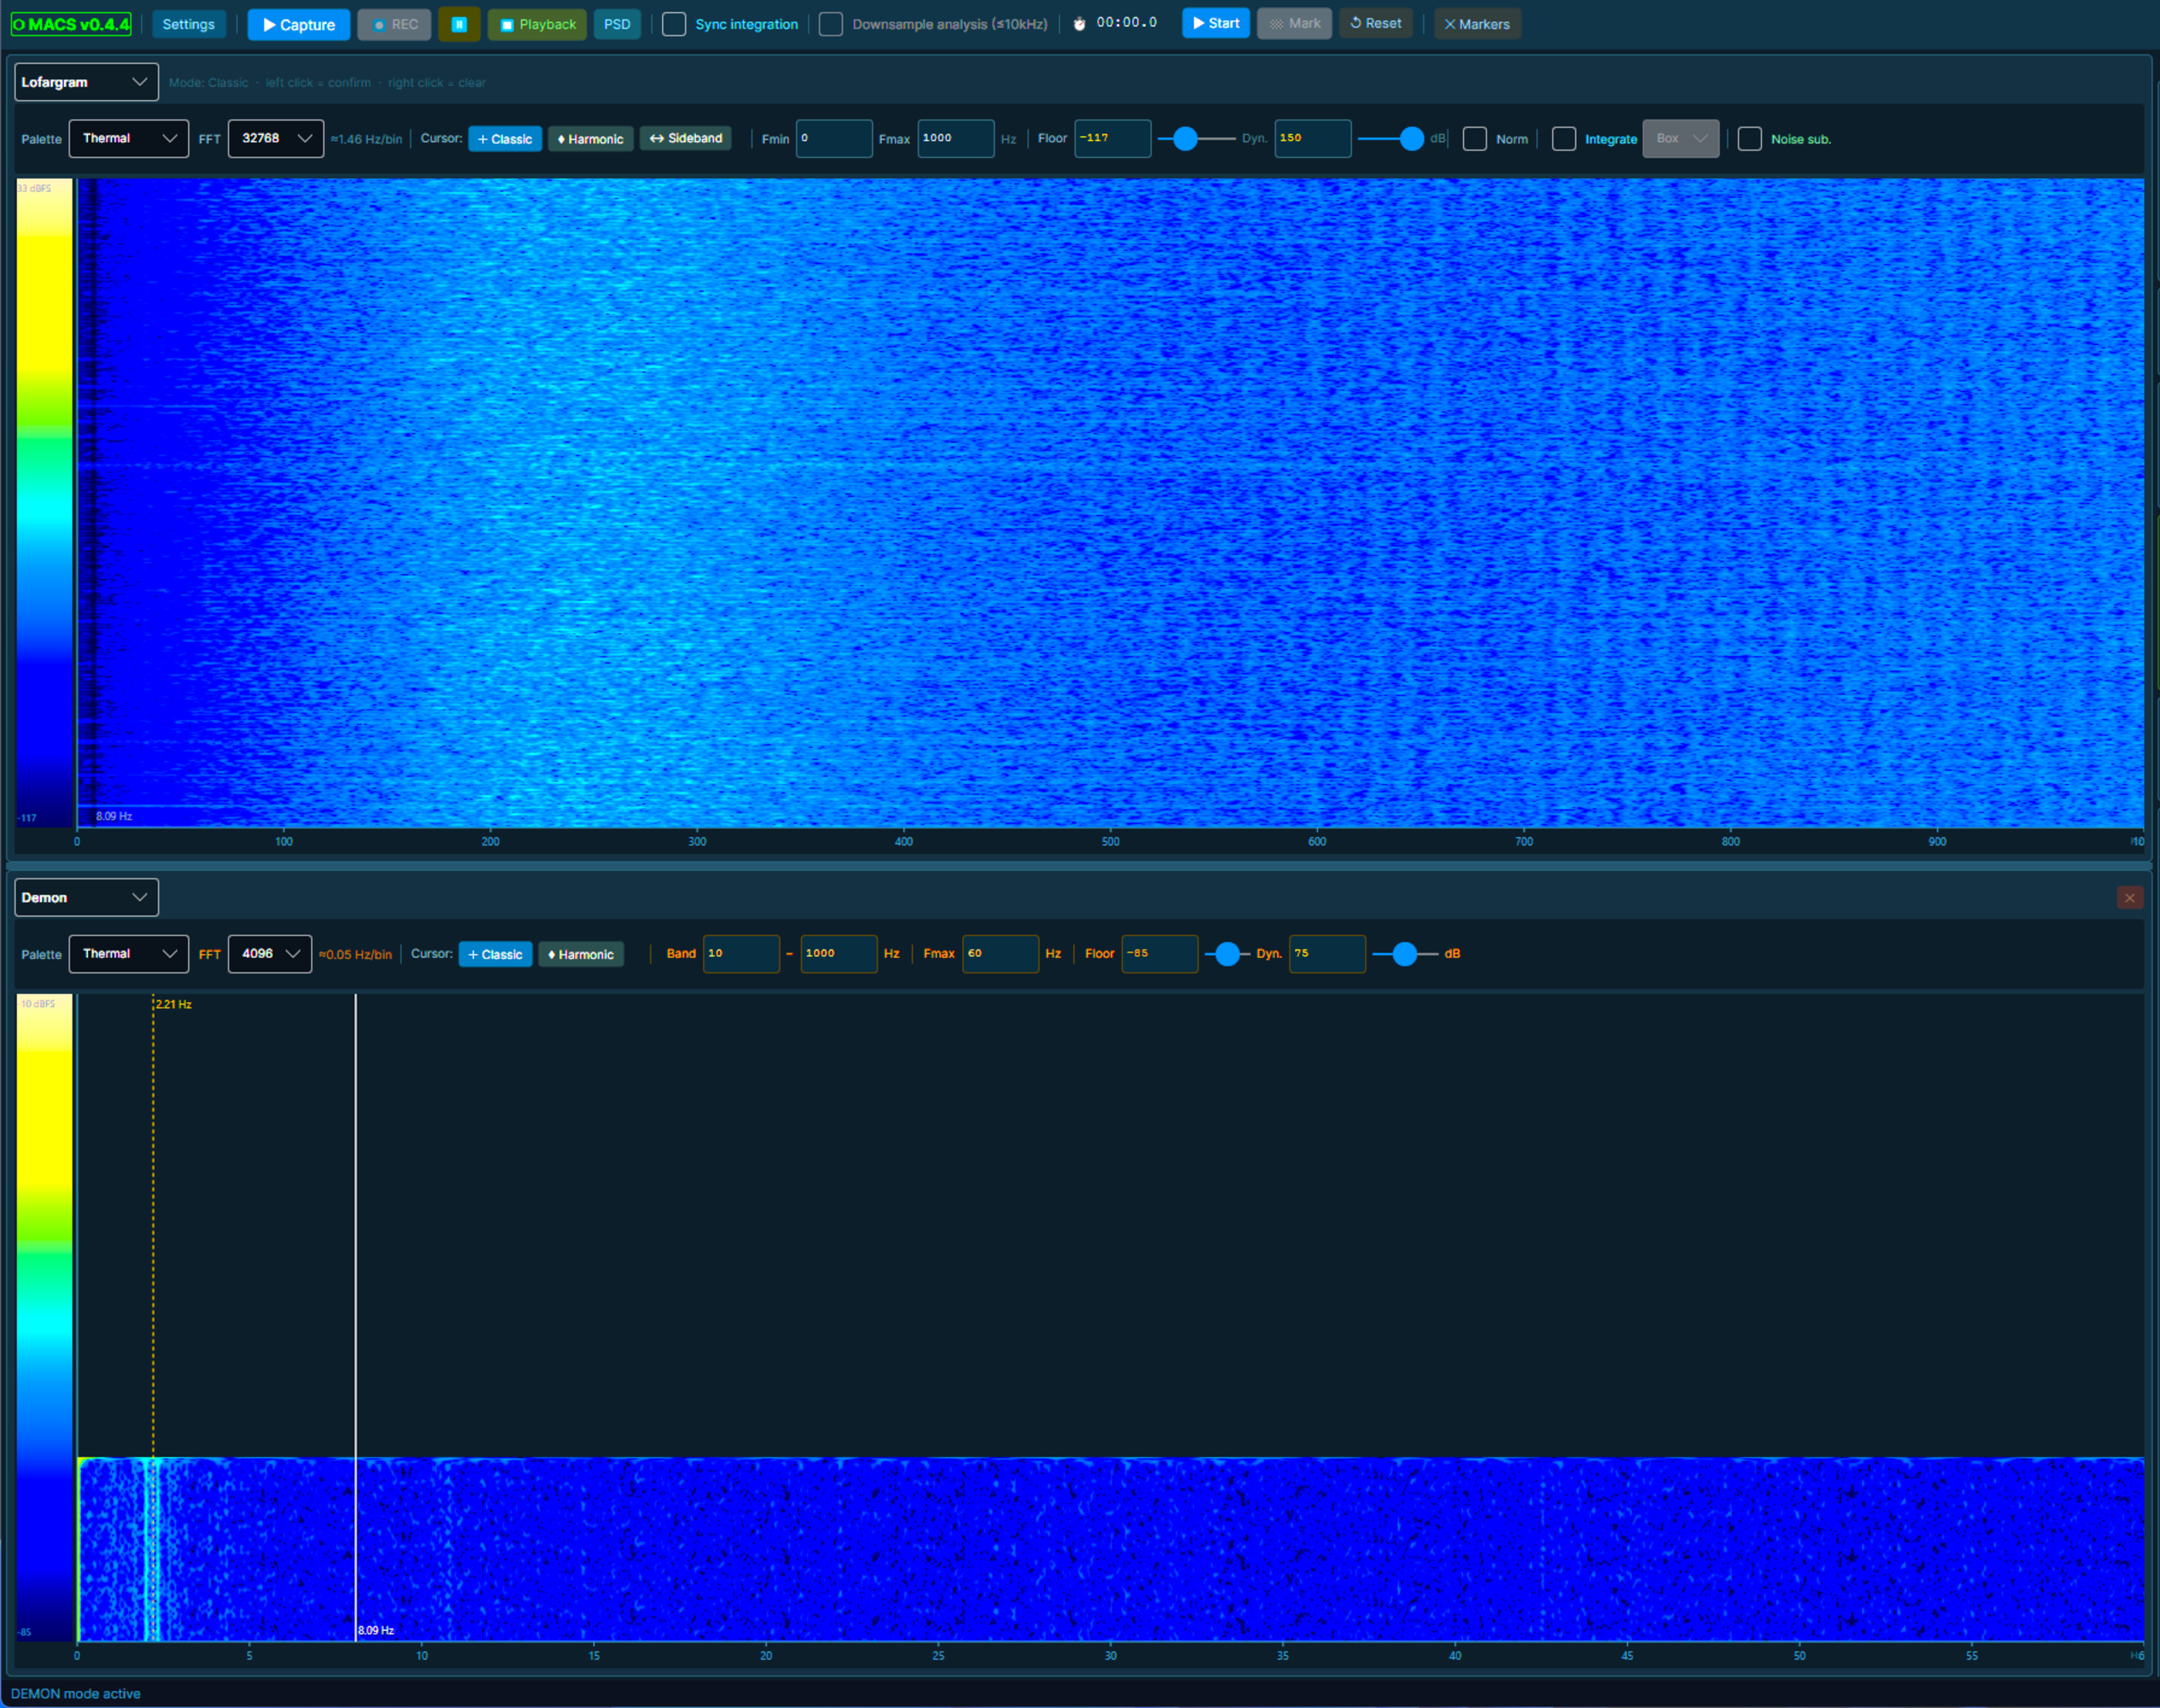
\includegraphics[width=300px]{../img/actuals/Type55_05.pdf}
	\caption{DEMON}
\end{figure}

There are also indications of higher tonals which fall very closely on the harmonics of the blade rate at 11 Hz. The third harmonic would be about 33 Hz and would be reinforced by the shaft harmonic. This is pure speculation but is a possible explanation for the faint line at 33 Hz.

\textbf{Classification}

We have enough information now to posit a classification for this vessel, which we will classify as potential warship, confirmed by spectral analysis.

\begin{compactenum}
    \item 5 blades with a high pitch turbine
    \item No diesel audio
    \item Broad noise bands
    \item Lack of sound usually associated with diesel engines
\end{compactenum}


Four ships in the recognition database match the noise band and 33 Hz signature

\begin{compactenum}
    \item Fuyu AOR: 22.3 kts at 134 RPM
    \item Ticonderoga CG: 24.2 kts at 134 RPM
    \item Renhai Type 055 DDG: 18.9 kts at 134 RPM
    \item Arleigh Burke DDG: 20 kts at 134 RPM
\end{compactenum}


Speed estimates are calculated from $SR \times (Max Speed \div Max RPM)$ (found from the recognition manual)

All three exhibit a very faint tonals around 30 - 34 Hz and a moderate noise band in the correct position.

For the Arleigh Burke the reported noise band and 30 Hz tonal are supposed to look much stronger. This questions this attribution suggesting medium confidence The Fuyu would be close to max speed (22 kts) at this SR which makes this a less likely candidate. Likewise a Ticonderoga would also be 10 kts below its maximum which would tend to suggest the diffuse noise band would be broader and more prominent.

\textbf{On the balance of probabilities the best fit based on the information we have is that our target is a Type 055 Renhai.}

\subsection{Illustrated Example 2: LOFAR - DEMON - Cepstrum}
\large Difficulty Rating \includegraphics{../img/actuals/Stars/"3 Stars.jpg"}

\begin{advisory}
    \textbf{Note: }Figures 22 - 27 were produced by the simulation engine not MACS. The equivalent MACS images are included in the download package.
\end{advisory}

This exercise demonstrates how a relatively complicated acoustic signal can be examined through three complementary forms of analysis: LOFAR, DEMON and cepstrum. Each technique approaches the signal differently. More importantly, the observations can be compared with one another and with the mathematical relationships expected from rotating machinery.

\textbf{Set Up:}
\begin{compactenum}
    \item Download and extract \texttt{"IE2 LOFAR DEMON Cepstrum.zip"}
    \item You should have the following directory structure.
    \begin{compactitem}
        \item csv
        \item img
        \item matlab
        \item python
        \item sound
    \end{compactitem}
    \item Using the matlab and python programs is discussed in Appendix D
\end{compactenum}

\textbf{Signal characteristics: }The supplied WAV has known parameters:
\begin{compactitem}
    \item Sample rate: 4,000 Hz
    \item Duration: 60 seconds
    \item Mean shaft rate: 1.30 Hz
    \item Shaft speed: 78 rpm
    \item Propeller blades: 5
    \item Blade rate: 6.50 Hz
    \item Second blade-rate harmonic: 13.00 Hz
    \item Machinery carriers: 150, 310, 620 and 900 Hz
    \item Additional machinery tonals: 48 and 96 Hz
\end{compactitem}

The relationship is: $\text{Shaft speed} = 60 \times 1.30 = 78\ \mathrm{rpm}$ and: $\text{Blade rate} = 5 \times 1.30 = 6.50\ \mathrm{Hz}$. A small ±0.025 Hz shaft-rate variation is included so the signal is not unrealistically perfect. Since we know what the two major fundamentals are the aim of the exercise is to see whether the three forms of analysis can recover them.

The synthetic example represents a five-bladed propeller turning at a Shaft Rate (SR) of 1.30 Hz, equivalent to 78 RPM. Its corresponding Blade Rate (BR) is therefore 6.50 Hz, with further related structure at multiples such as 13.00 Hz.

The objective is not simply to find those numbers in a graph. The exercise demonstrates the reasoning process by which several apparently different observations may be recognised as manifestations of the same underlying mechanical process.

\subsubsection{The Waveform}

The first image shows the acoustic waveform in the time domain.

\begin{figure}[h]
	\centering
	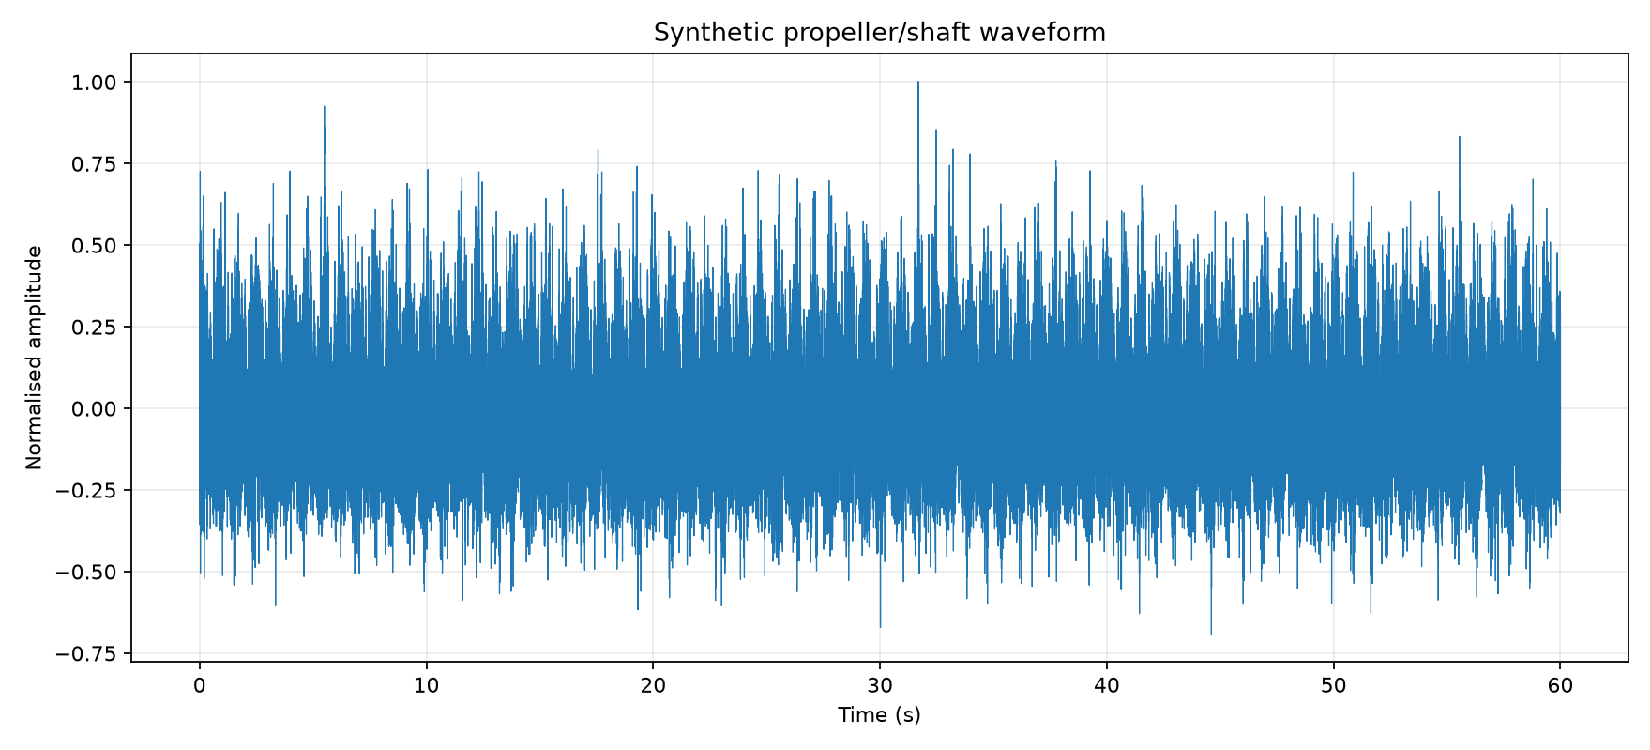
\includegraphics[width=350px]{../img/actuals/01_waveform.pdf}
	\caption{The Waveform}
\end{figure}

At this stage, the complete signal is represented as amplitude against time. Although the waveform confirms the presence and evolution of acoustic energy, most of the useful mechanical relationships are difficult to determine directly by eye. This is an important starting point. Information can be present in a signal without being visually obvious in the time waveform. The remaining analyses therefore transform or process the same underlying information to make particular characteristics easier to observe.

\subsubsection{The LOFAR Spectrogram}

The second image introduces frequency as a major analytical dimension.

\begin{figure}[h]
	\centering
	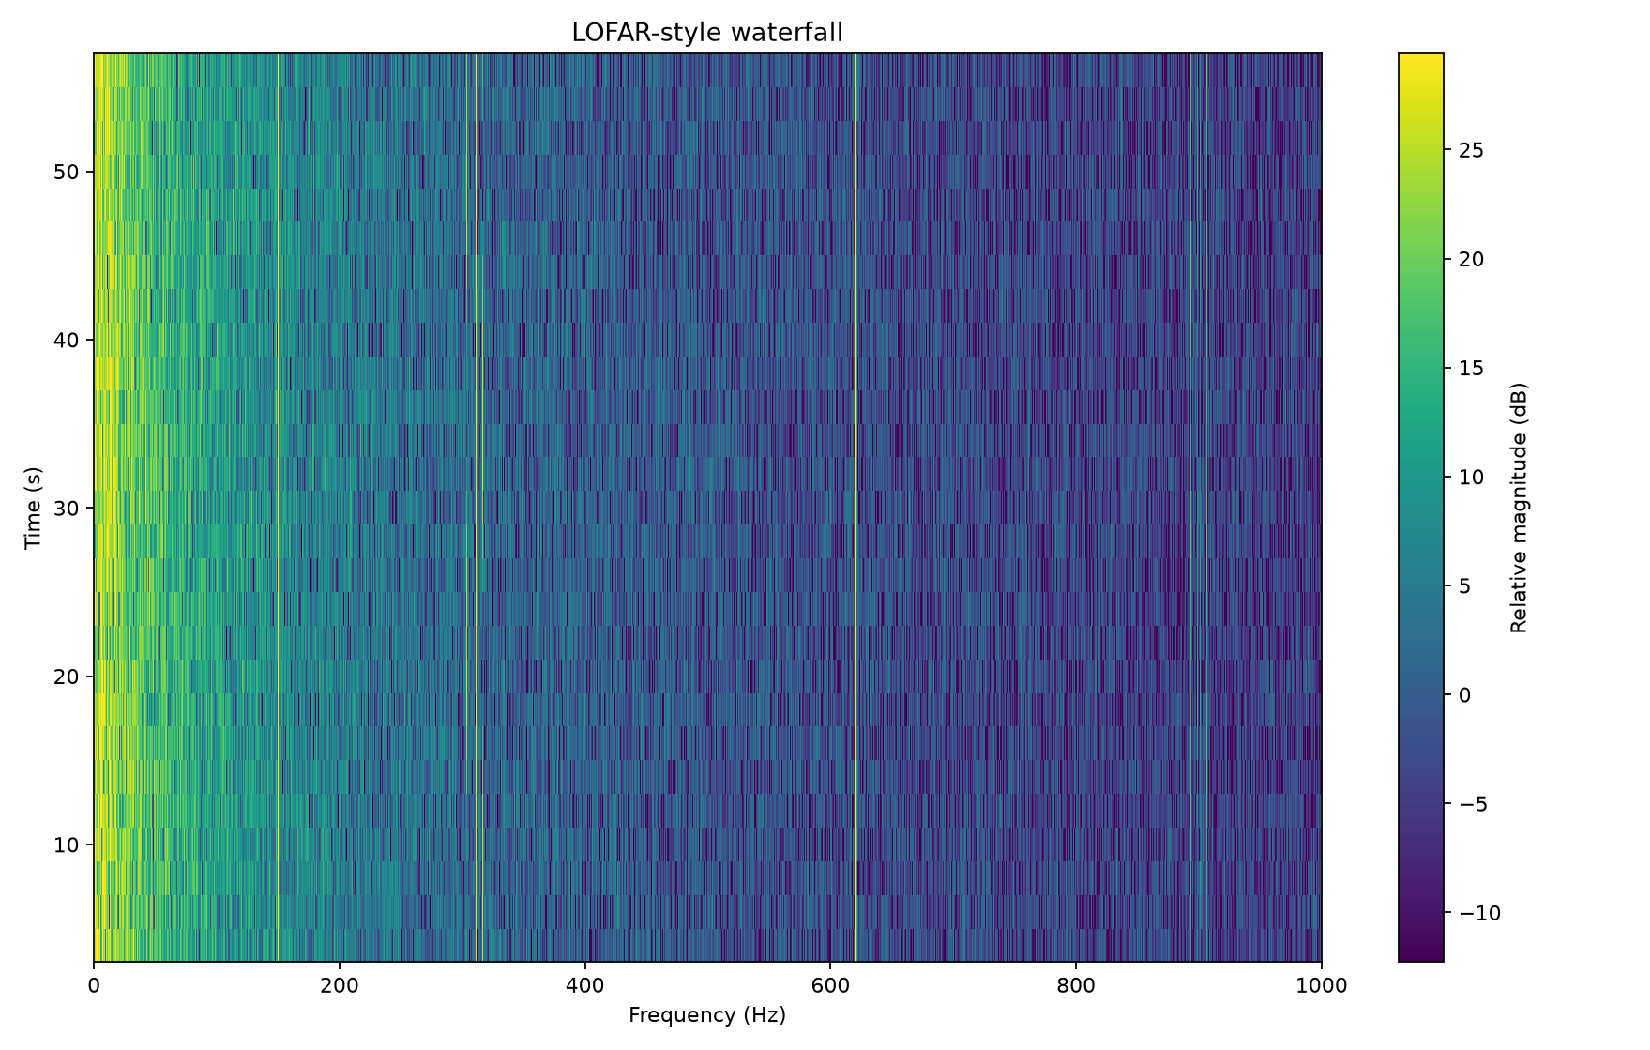
\includegraphics[width=350px]{../img/actuals/02_lofar_spectrogram.pdf}
	\caption{LOFAR Waterfall}
\end{figure}

The LOFAR-style display shows frequency against time, with intensity indicating the relative strength of spectral components. Persistent tonal components consequently appear differently from broadband energy or components that vary with time.

LOFAR asks: What frequency components are present, and how persistent are they?

This is the first move from observing a complex acoustic waveform towards identifying structure within it. The synthetic signal contains machinery-related frequencies and modulated carrier energy. LOFAR therefore provides evidence of the signal's spectral organisation. It can show tonals, harmonics and potentially the effects of modulation around stronger components. However, the presence of a frequency line does not by itself establish what produced it. The MACS review specifically identifies this distinction as important: a tonal peak is not automatically machinery. LOFAR therefore supplies the spectral evidence, but interpretation requires further corroboration.

\subsubsection{The Mean LOFAR Spectrum}

The third image collapses the time dimension by averaging the LOFAR spectra.

\begin{figure}[h]
	\centering
	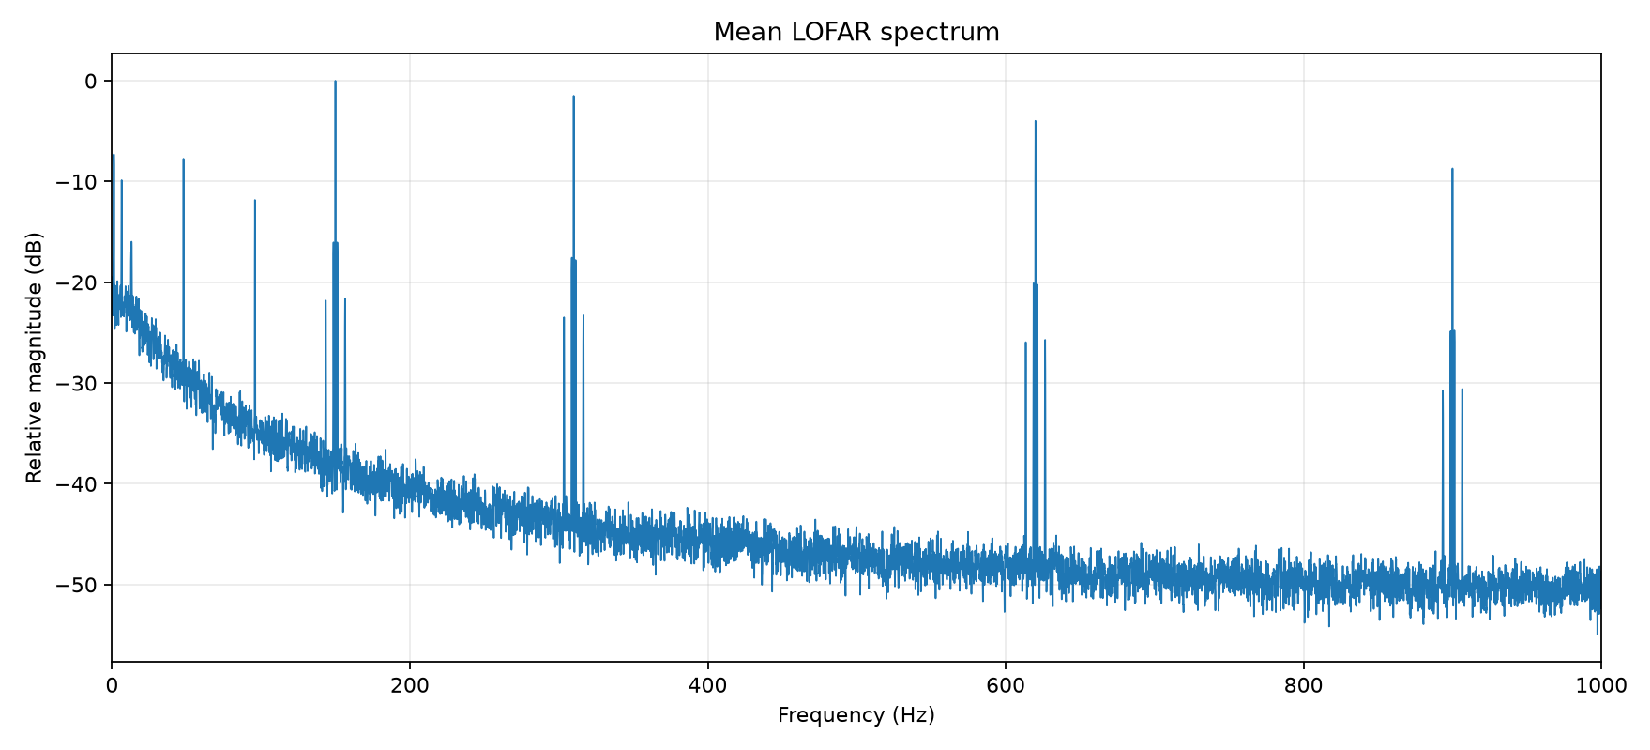
\includegraphics[width=350px]{../img/actuals/03_mean_lofar_spectrum.pdf}
	\caption{Mean LOFAR Spectrum}
\end{figure}

The result makes persistent frequencies easier to inspect quantitatively. The distinction between Images 2 and 3 is useful:

 \begin{compactitem}
    \item The LOFAR spectrogram answers when and where spectral energy occurs;
    \item The mean spectrum emphasises which spectral components persist strongly across the observation.
 \end{compactitem}


A peak in the mean spectrum is consequently an analytical clue rather than an automatic identification. Relationships between peaks matter considerably more. If components show harmonic spacing, sideband relationships or other regular structure, the analyst has a basis for asking whether they share a common mechanical origin.

This naturally leads to DEMON analysis.

\subsubsection{The DEMONgram}

DEMON provides a fundamentally different view of the signal.

\begin{figure}[h]
	\centering
	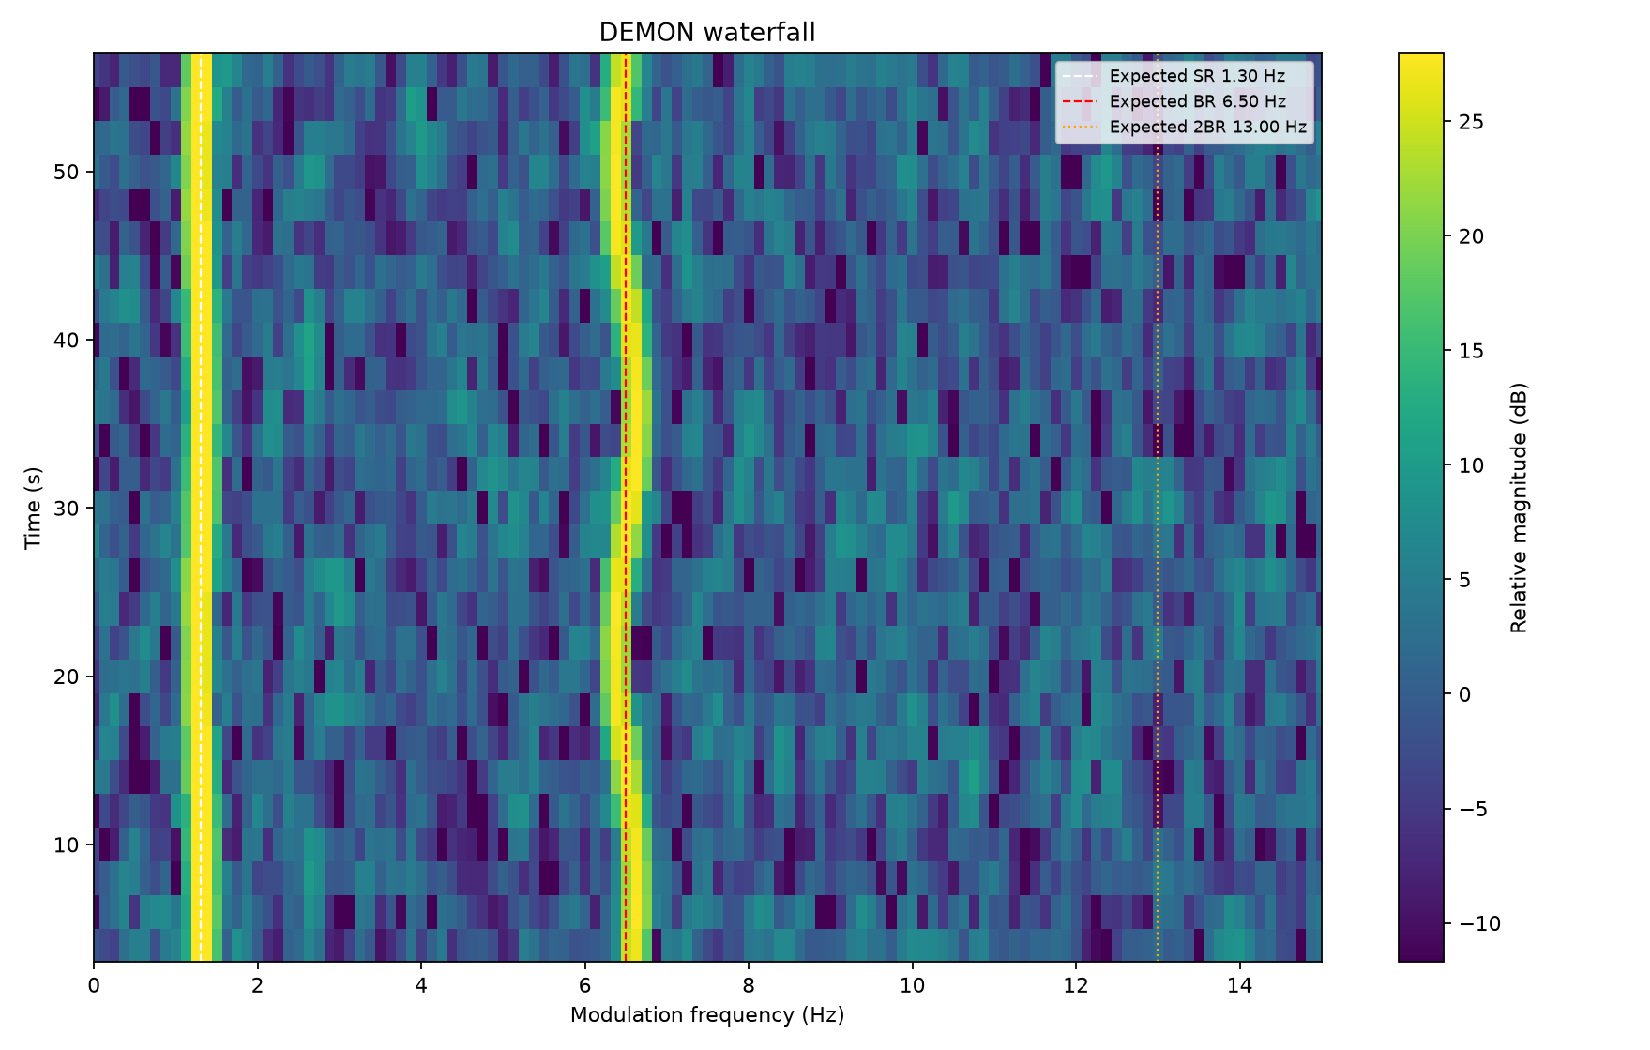
\includegraphics[width=350px]{../img/actuals/04_demongram.pdf}
	\caption{DEMON Waterfall}
\end{figure}

Rather than simply asking which acoustic frequencies are present, DEMON examines periodic amplitude modulation within a selected acoustic band. This distinction is fundamental and was specifically highlighted as a strength in the review of the MACS material: DEMON extracts modulation frequencies, which are subsequently interpreted through shaft and blade relationships.

The DEMONgram therefore asks: At what rates is the acoustic energy being modulated, and how do those rates behave with time?

That question is particularly relevant to rotating machinery.

In the synthetic example there is a known Shaft Rate:

$SR=1.30\text{ Hz}$

and a five-bladed propeller.

The corresponding Blade Rate is therefore:

$BR=B\times SR$

where BB is the number of blades.

Thus:

$BR=5\times1.30=6.50\text{ Hz}$

The DEMON display allows those low-frequency modulation relationships to become much more apparent than they may have been in the original waveform or conventional spectral display.

\subsubsection{The Mean DEMON Spectrum}

The fifth image is particularly useful for interpretation because it converts the DEMONgram into an averaged modulation spectrum. The principal frequencies of interest are:

$1.30\text{ Hz},\quad6.50\text{ Hz},\quad13.00\text{ Hz}$

These are not three arbitrary numbers, they form a mathematically related family.
\begin{figure}[h]
	\centering
	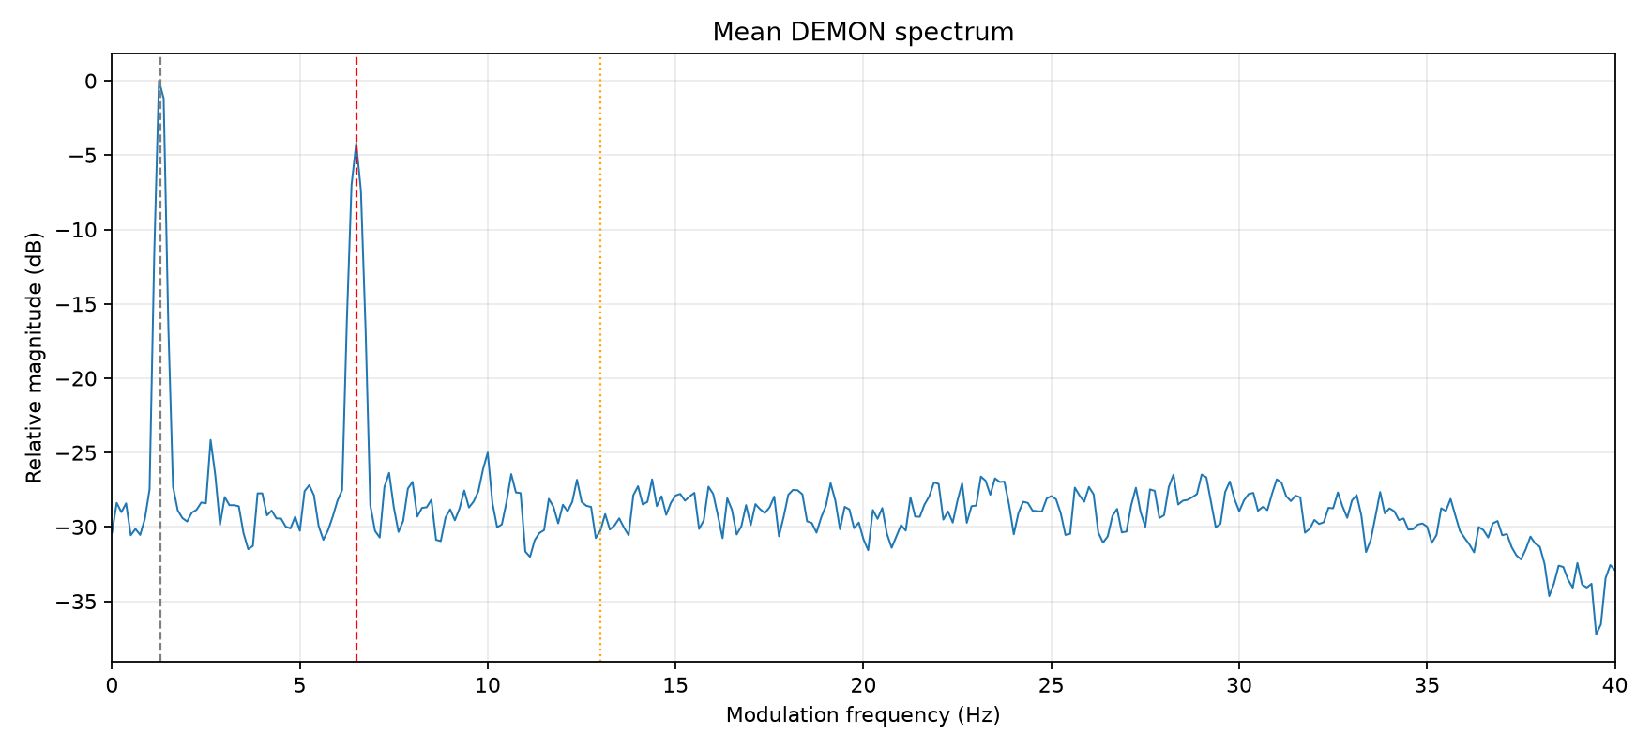
\includegraphics[width=350px]{../img/actuals/05_mean_demon_spectrum.pdf}
	\caption{Mean DEMON spectrum}
\end{figure}

\begin{advisory}
\textbf{Why the 13 Hz line is unclear: }The second Blade Rate harmonic is not convincingly visible in the supplied DEMONgram. That is a limitation of the synthetic signal rather than something that should be explained away in the guide.
\end{advisory}

The 1.30 Hz component corresponds to the known Shaft Rate, while:

$\frac{6.50}{1.30}=5$

This is consistent with a five-bladed propeller.

Furthermore:

$13.00=2\times6.50$

so 13.00 Hz is consistent with the second harmonic of Blade Rate.

The value of the DEMON spectrum therefore lies not merely in finding a strong peak, but in recognising a coherent pattern:

$SR\rightarrow BR\rightarrow2BR$

That provides substantially more meaningful evidence than interpreting any one component alone.

\subsubsection{The Real Cepstrum}

The sixth image examines the signal from yet another perspective.

\begin{figure}[h]
	\centering
	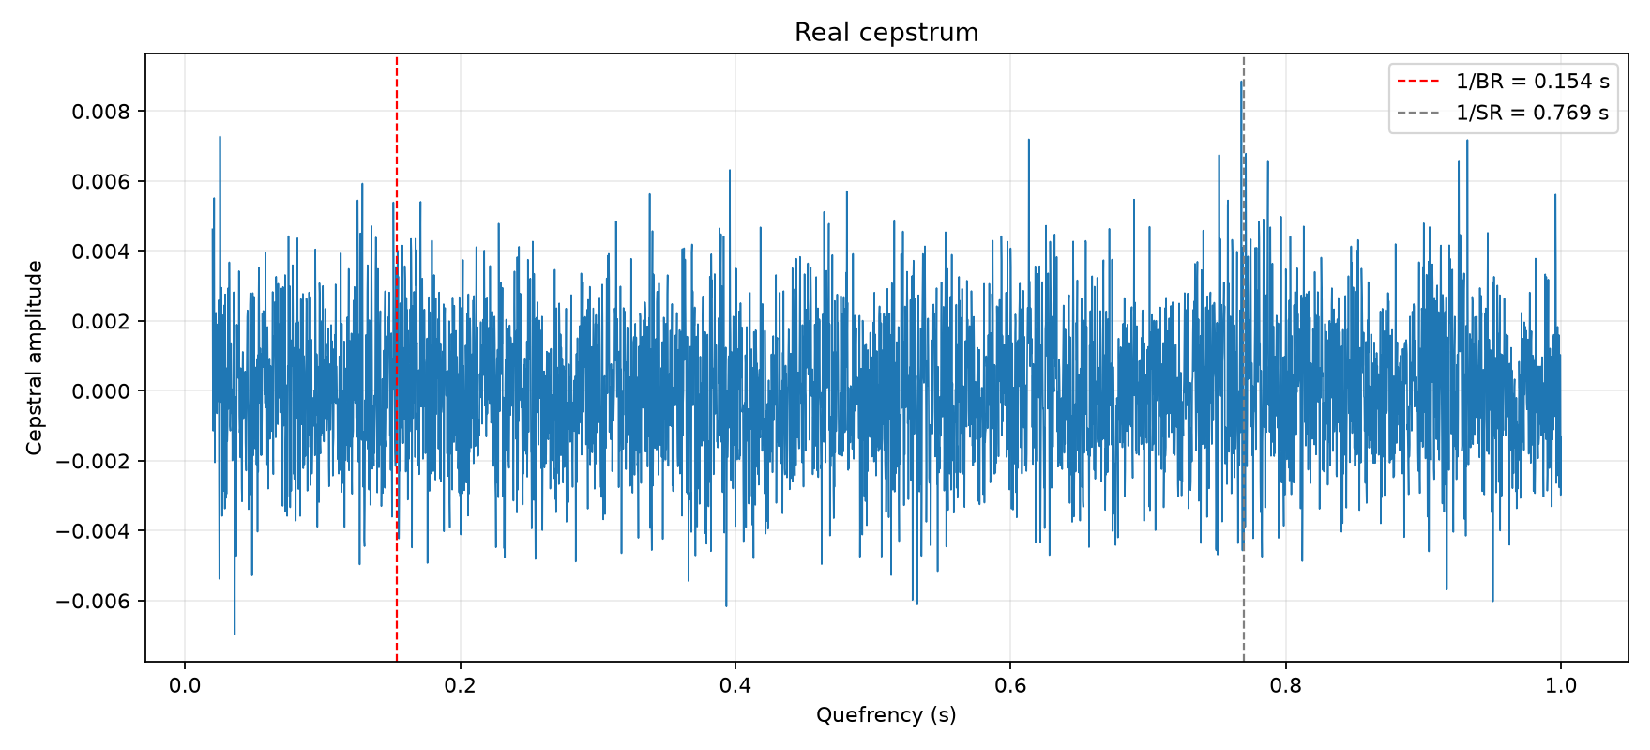
\includegraphics[width=350px]{../img/actuals/06_real_cepstrum.pdf}
	\caption{Real Cepstrum}
\end{figure}


Cepstral analysis is useful for revealing regular spectral spacing. Its horizontal coordinate is termed quefrency and has units of time.

The basic relationship is:

\[
    q=\frac{1}{\Delta f}
\]

where $\Delta f$ is a repeating frequency spacing.

For the 6.50 Hz Blade Rate relationship:

\[
    q=\frac{1}{6.50}\approx0.154\text{ s}
\]

For the 1.30 Hz shaft relationship:

\[
    q=\frac{1}{1.30}\approx0.769\text{ s}
\]

The significance of the cepstrum is therefore that it provides another way of searching for periodic organisation within the signal.

The real cepstrum contains numerous peaks because it responds to regular spacing anywhere in the acoustic spectrum. The vertical markers at 0.154 s and 0.769 s are expected quefrencies calculated from the Blade Rate and Shaft Rate estimated by DEMON. They are reference positions, not automatic detections. A peak at either position supports the interpretation only when it is locally prominent and agrees with independent LOFAR and DEMON evidence.

\begin{learnpoint}
    \textbf{Learning Point} \\
    You should be cautious in identifying 0.154 s and 0.769 s as BR and SR from this cepstrum alone. First obtain candidate rates from DEMON and supporting spectral structure from LOFAR, then uses the cepstrum to look for compatible periodic spacing. If the expected positions do not stand out locally, the cepstrum has not added strong corroborating evidence in that particular recording.
\end{learnpoint}


To summarise so far:

\begin{compactitem}
    \item \textbf{LOFAR} presents spectral structure.
    \item \textbf{DEMON} presents modulation structure.
    \item \textbf{CEPSTRUM} presents periodic spectral-spacing structure.
\end{compactitem}

When compatible relationships appear in these different representations, confidence in the interpretation can increase.

\begin{learnpoint}
    \textbf{Learning Point}\\
    No individual display needs to carry the whole interpretation. LOFAR may reveal persistent spectral features but leave their origin uncertain. DEMON may expose a family of modulation rates. The cepstrum may independently indicate corresponding periodic spacing. Mathematical relationships can then test whether these observations form a physically coherent pattern. This layered confirmation principle is the means by which an analyst avoids over-interpreting one attractive spectral peak.
\end{learnpoint}
\subsubsection{Correlating the Evidence}

This is the central purpose of the exercise.

The analytical progression can be thought of as:

\begin{figure}[h]
	\centering
	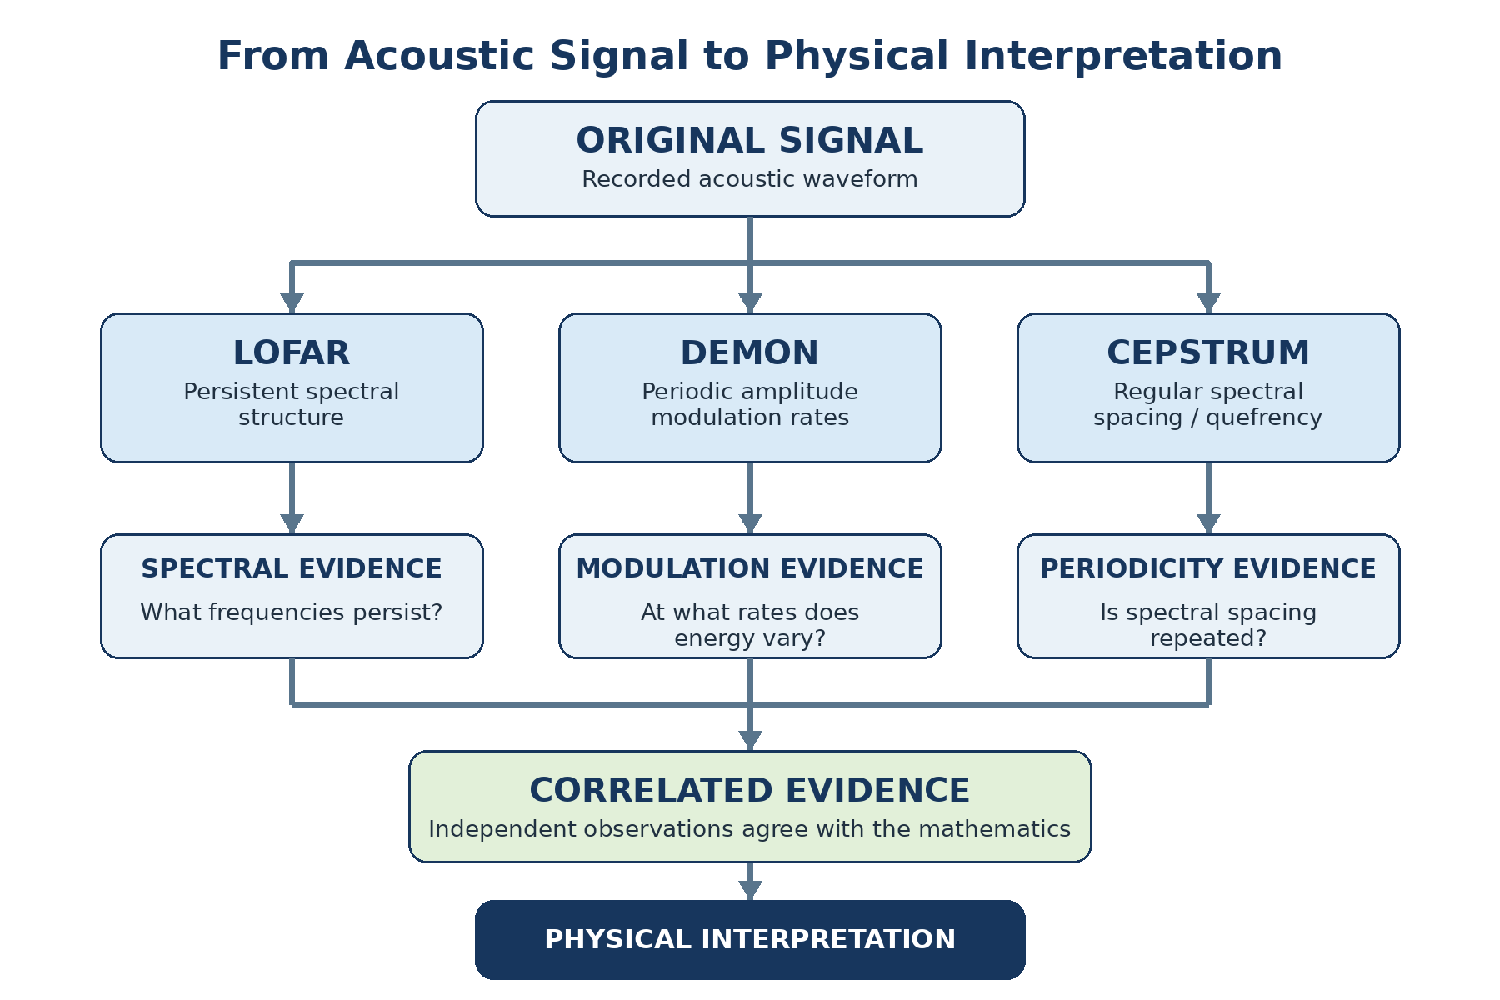
\includegraphics[width=350px]{../img/actuals/LDC_evidence_flow.pdf}
	\caption{LOFAR, DEMON, CEPSTRUM evidence flow}
\end{figure}



\subsubsection{Summary of Findings}

The synthetic example begins with a known:
\[
    \boxed{SR=1.30\text{ Hz}}
\]

Shaft frequency converts directly to rotational speed: $RPM=60\times SR$

therefore:
\begin{align*}
    RPM &= 60\times1.30 \\
    RPM &= \boxed{78 RPM}
\end{align*}

For five propeller blades: $BR=B\times SR$ and therefore:
\begin{align*}
    BR = 5\times1.30 \\
    \boxed{BR = 6.50\text{ Hz}}
\end{align*}

The next Blade Rate harmonic occurs at:
\begin{align*}
    BR = 2\times6.50 \\
    \boxed{BR = 13.00\text{ Hz}}
\end{align*}
    
Conversely, if SR and BR were measured without knowing the blade count:
\begin{align*}
    B &= \frac{BR}{SR} \\[1ex]
    B &= \frac{6.50}{1.30} \\[1ex]
    B &= \boxed{5}
\end{align*}

Finally, the corresponding reciprocal relationships provide expected cepstral quefrencies:
\[
    q_{BR}=\frac{1}{6.50}\approx\boxed{0.154\text{ s}}
\]

and:
\[
    q_{SR}=\frac{1}{1.30}\approx\boxed{0.769\text{ s}}
\]

The exercise therefore brings the analysis full circle. LOFAR identifies spectral structure, DEMON exposes modulation structure, and the cepstrum searches for periodic spectral spacing. The mathematical relationships between Shaft Rate, rotational speed, Blade Rate, harmonics and quefrency then provide a common framework within which those observations can be compared.

The important finding is consequently not simply “there is a peak at 6.5 Hz”. It is the much stronger chain of reasoning:
\[
    \boxed{ 1.30\text{ Hz} \rightarrow 78\text{ RPM} \rightarrow 5\times1.30 \rightarrow 6.50\text{ Hz} \rightarrow 2\times6.50 \rightarrow 13.00\text{ Hz} }
\]

supported by complementary views of the same underlying signal.

\begin{learnpoint}
    \textbf{Learning Point:}\\
    This exercise demonstrates that acoustic analysis becomes most persuasive when observations from different analytical domains agree with one another and with the underlying mathematics, rather than when an interpretation depends upon a single conspicuous peak. This reflects the broader principle that the evidence should support the hypothesis. That fits with the MACS Guide's broader analytical approach: LOFAR asks what spectral structure exists, DEMON reveals modulation behaviour, and the cepstrum looks for compatible periodic spacing. The interpretation becomes more concrete when those independent observations agree with the underlying physics and mathematics
\end{learnpoint}

\subsection{Exercise 1: Finding the way}
\textcolor{commentGreen}{*** WIP ***}

This exercise is to help you find your way around MACS, identify fundamental tonals and to optimize settings.

\subsection{Exercise 2: Sabre Dance}
\begin{compactenum}
    \item Download and extract \texttt{"Sabre Dance".zip}
    \item Carefully read the exercise \texttt{Outline.pdf} and then follow the instructions
\end{compactenum}

\subsection{Exercise 3: Snaky Medusa}
\textcolor{commentGreen}{*** WIP ***}
\begin{compactenum}
    \item Download and extract \texttt{"Snaky Medusa".zip}
    \item Carefully read the exercise \texttt{Outline.pdf} and then follow the instructions
\end{compactenum}

\subsection{Exercise 4: Classification \#1}
\begin{compactenum}
    \item Download and extract \texttt{"EX4 Classification 1".zip}
    \item Carefully read the exercise \texttt{Outline.pdf} and then follow the instructions
\end{compactenum}

\subsection{Exercise 5: Classification \#2}
\begin{compactenum}
    \item Download and extract \texttt{"EX5 Classification 2".zip}
    \item Carefully read the exercise \texttt{Outline.pdf} and then follow the instructions
\end{compactenum}

\subsection{Final Test}
\begin{compactenum}
    \item Download and extract \texttt{"Exam Distribution".zip}
    \item Carefully read the exercise \texttt{Exam Outline.pdf} and then follow the instructions
\end{compactenum}

\pagebreak

\section{Tools}
\textcolor{commentGreen}{*** WIP ***}

\subsection{Range Predictor}

\subsection{Sonification}

\subsubsection{Sonification Training}

\subsection{Own Ship Target Diagram}

\subsection{Environment}

\textbf{Page Intentionally Left Blank}
\pagebreak
\section{References}
\label{sec:References}
\textcolor{commentGreen}{*** WIP ***}

\textbf{Page Intentionally Left Blank}

\pagebreak

\section{Appendix A - A Casual Guide To Sound, SONAR and FFT}
\label{sec:Appendix_A}
\subsection{Sound a short Introduction}

\textit{Why are ears different from eyes?}

When we learn about sound we are often taught that sound travels in waves. Later on we learn that light travels in waves too (and as particles, but that’s another story). You may have been shown an oscilloscope with sound represented as a beautiful sine wave sometimes accompanied by a pure note. That’s all well and good, but this is not how sound should be understood. The problem with viewing light and sound as comparable waves is that they are not comparable at all. Sound is physical touching. Imagine a line of billiard balls lined up on the table. If you bump the very first ball, that ball hits the next one, which hits the next one, down the line. The balls themselves do not travel across the table. Only the push or the energy travels. So the important takeaway here is that sound needs a medium, something to travel through (like air, water, or solid things). Light, on the other hand, is a form of electromagnetism (energy made of electrical and magnetic fields moving together).

\begin{wrapfigure}[25]{r}{0.3\textwidth}
    \centering
        \vspace{-10pt}
        \includegraphics[width=\linewidth]{../img/actuals/Shouting.pdf}
\end{wrapfigure}

Electromagnetic waves can travel without a medium which is why you can see the sun and the stars even though there is a vacuum between us and them (top tip: don’t look at the sun without good protection or sound will likely be the only waves you will experience afterwards). Light is like energy rays travelling through space it doesn’t need air, water, or anything else. So, what else is different between sound and light? The biggest difference is the speed at which they travel. Light is fast, so fast that nothing in the universe will ever be faster. Light travels at 186,282 miles per second or 299,792.458 kilometres per second. More usefully that’s about 1.8 x 10¹² furlongs per fortnight. Sound on the other hand travels much more slowly. In air at 20°C (68°F) sound travels at 762 miles per hour or 1,235 kilometres per hour. Interestingly from our perspective, is sound’s behaviour in water where it travels much faster, 3,310 mph or 5,330 kph. Sound can also do weird things in water depending on temperature, salinity and pressure.

This is useful for submariners because they can exploit these phenomena to hide a submarine’s sound from other submarines, surface ships and sonobuoys.

So to answer our starting problem about ears and eyes. Both have evolved to pick up waves. In the case of ears it’s mechanical movement of the eardrum and ear bones that capture the push from sound which our brain then interprets as sound. Our eyes, on the other hand, evolved to detect electromagnetic waves which our brain converts into images. Two waves two supremely evolved organs.

\subsection{SONAR}

\textit{Why do I need SONAR, I'm not a bat?}

We’ve all watched movies with submariners nervously listening to an approaching destroyer just waiting for that first sonar PING! It’s so ingrained that it has literally become a movie meme, but what actually is SONAR?

SONAR stands for Sound Navigation And Ranging. You may think that the technology is modern, but the first documented person to use it was Leonardo da Vinci in 1490; he dipped a tube underwater so he could listen to approaching ships.

SONAR comes in two types active and passive. Submarines need SONAR because when it’s underwater the crew can not see what’s around them. Sound becomes the submarines eyes just like a bat navigating its way in a pitch black cave.

Active SONAR uses systems to emit sound, the ping we all know. The sound travels and bounces off anything nearby. The system listens to these echoes and then by knowing the speed of sound in water produces a range to the target. By generating echoes from different angles SONAR can also locate the target. Submarines tend not to use active sonar for the simple reason that the noise also gives away their position and location. Not a very good idea in a combat situation. There are some circumstances when a submarine may use active sonar. In MNW these are the fathometer and the high frequency SONAR. In game these are undetectable by the enemy but in real life this may be different.

\begin{wrapfigure}[11]{l}{0.5\textwidth}
    \centering
    \vspace{-10pt}
    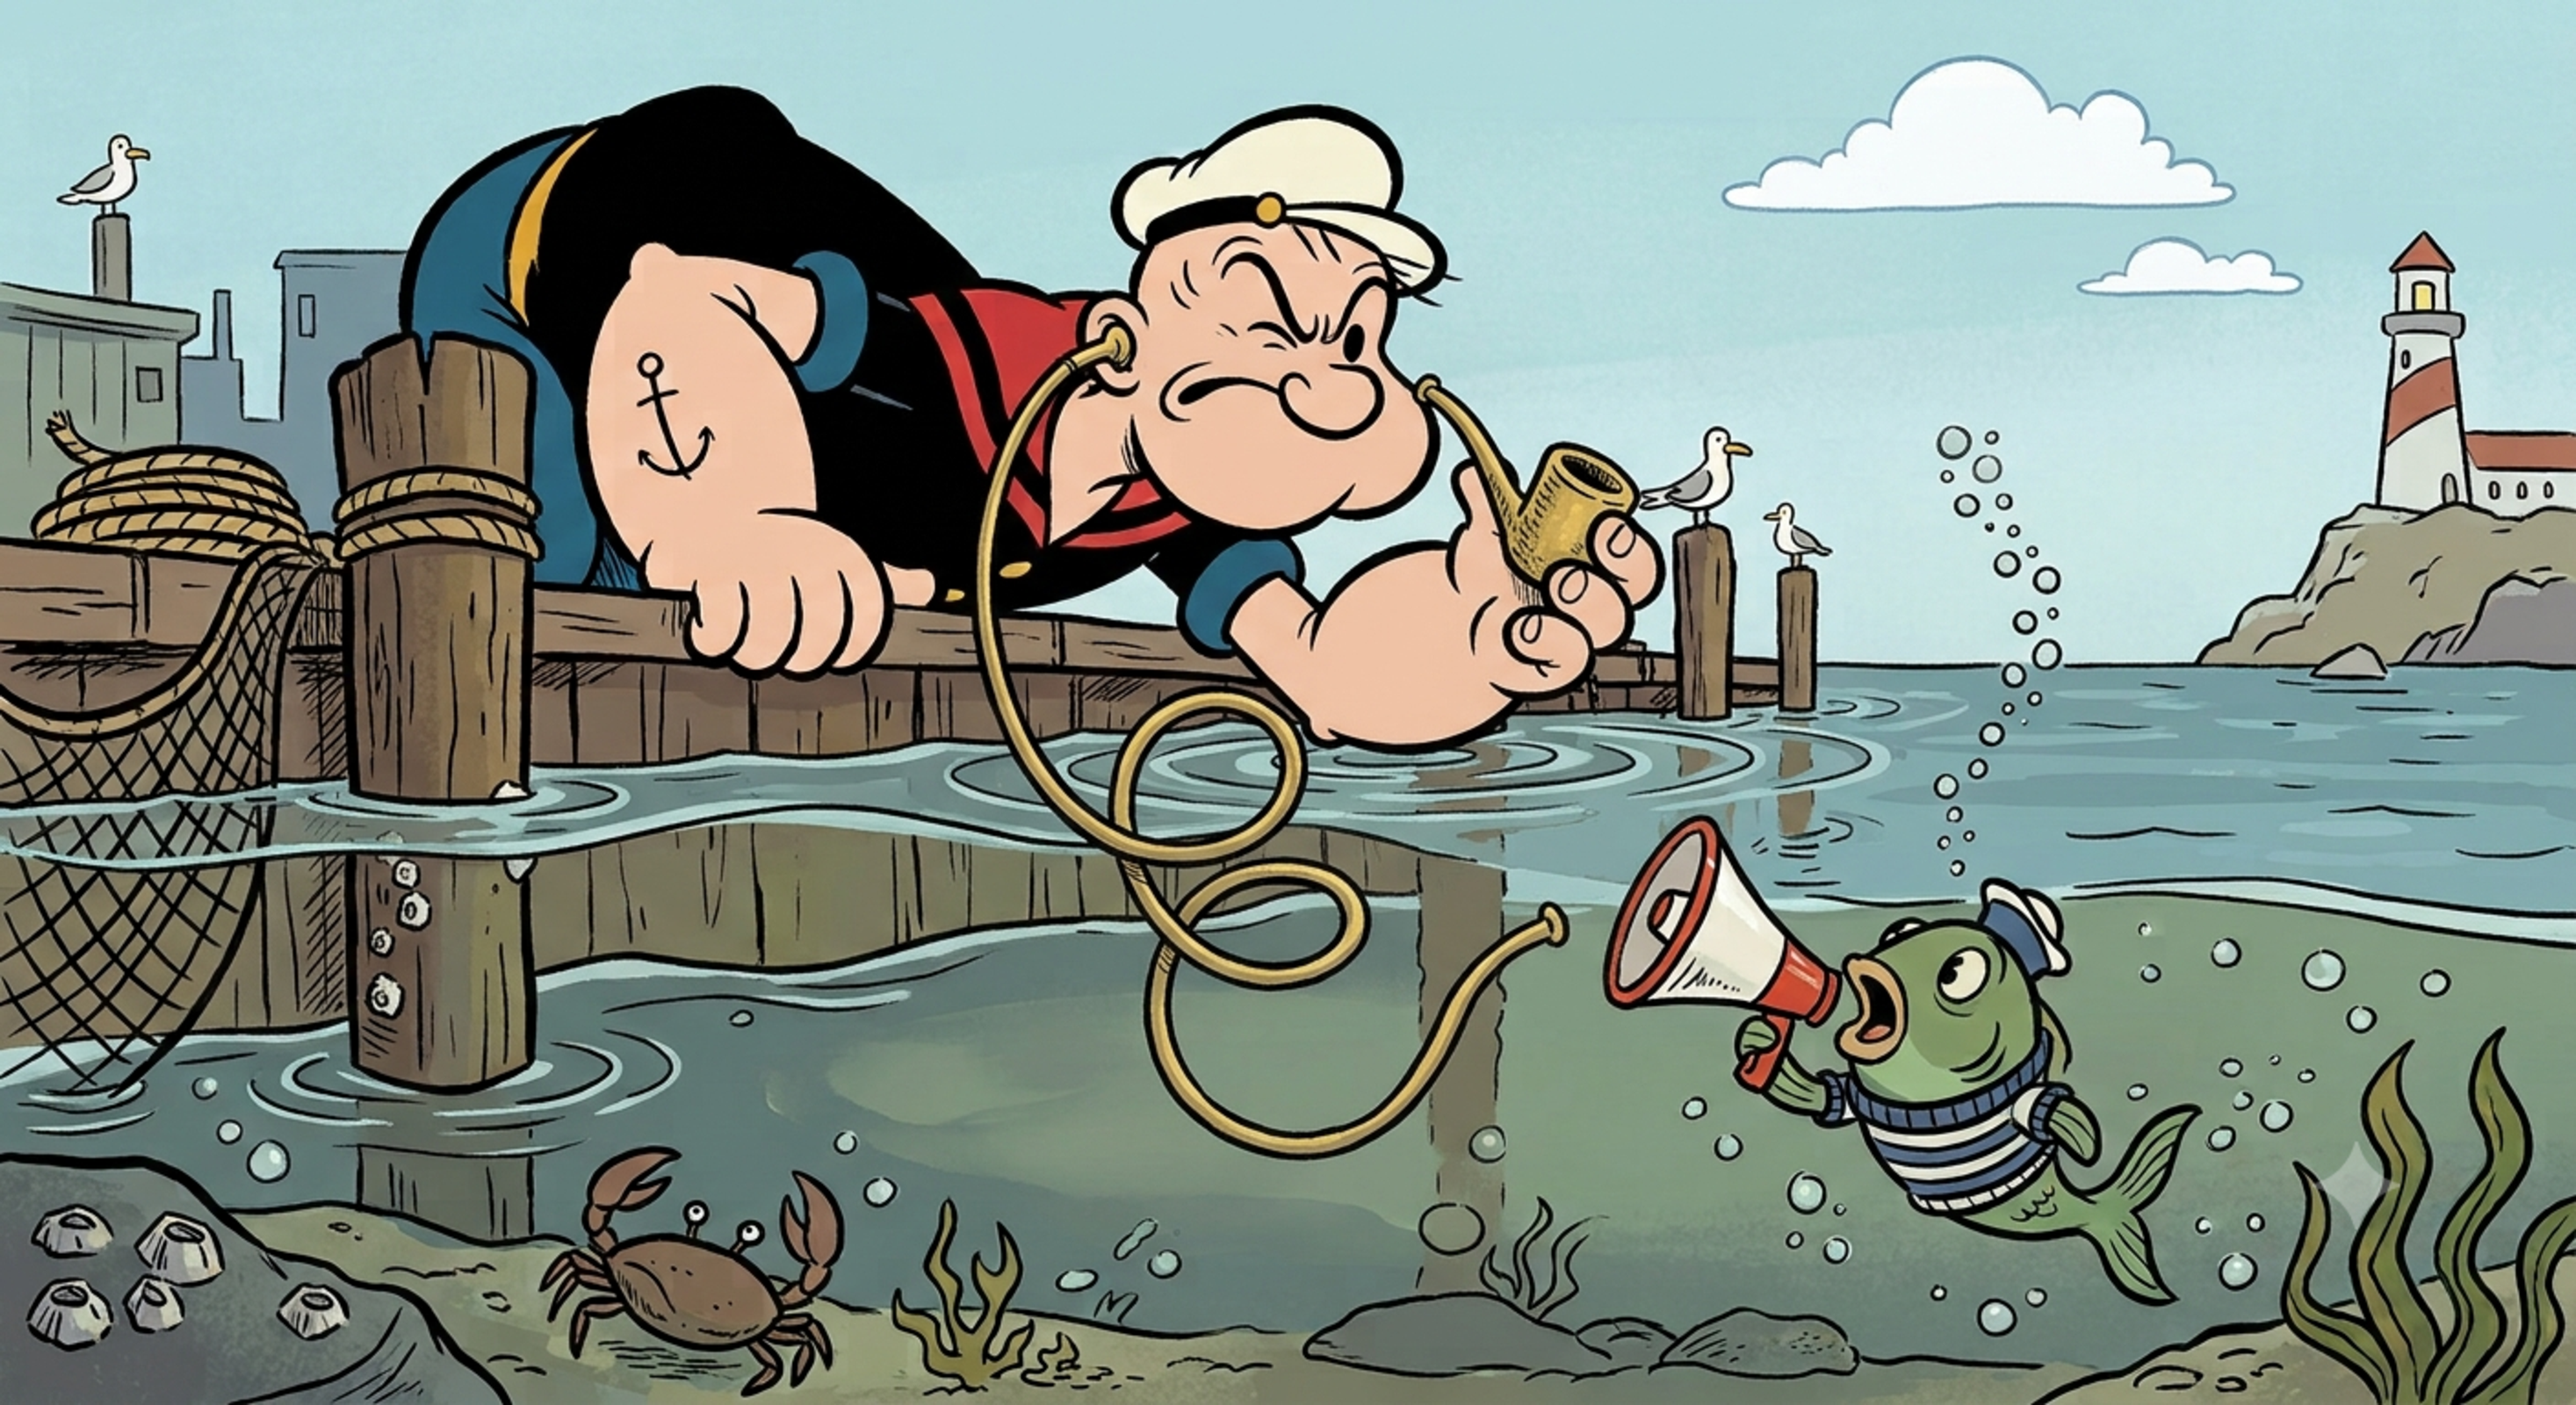
\includegraphics[width=\linewidth]{../img/actuals/sonar.pdf}
\end{wrapfigure}

Passive sonar is where the fun starts. With this a submarine crew can listen to what’s going on around them. By listening to other subs and ships the crew can determine speed, bearing and often the identity of the target, without giving away your own location. In MNW you have many of the tools that real submariners have. Using these tools you can make educated guesses as to what you are listening to, where it is and how fast it is. Putting all of this together, means you can stealthily avoid an enemy or plan an attack.

MACS allows you to do a more refined version of the sound analysis which may help you in game. You can run MACS alongside MNW, and it will take the sound generated by the in game SONAR system and give you a detailed LOFAR and DEMON analysis which you can use to complement the in game experience. Running MACS with the game is explained in Appendix X.

\subsection{What the FFT?}

\textit{Oh no! It's Math Class}

When you or the SONAR system hears (detects) a natural sound that sound is not just a single waveform. Think of a chord played on a piano, it sounds like one thing but is actually several notes played together. The Fast Fourier Transform (FFT) is a clever way to break a complicated signal into the frequencies that make it up. FFT takes the combined sound in the chord and tells you:

\begin{wrapfigure}[7]{r}{0.5\textwidth}
    \setlength{\intextsep}{0pt}
    \centering
    \vspace{-45pt}
    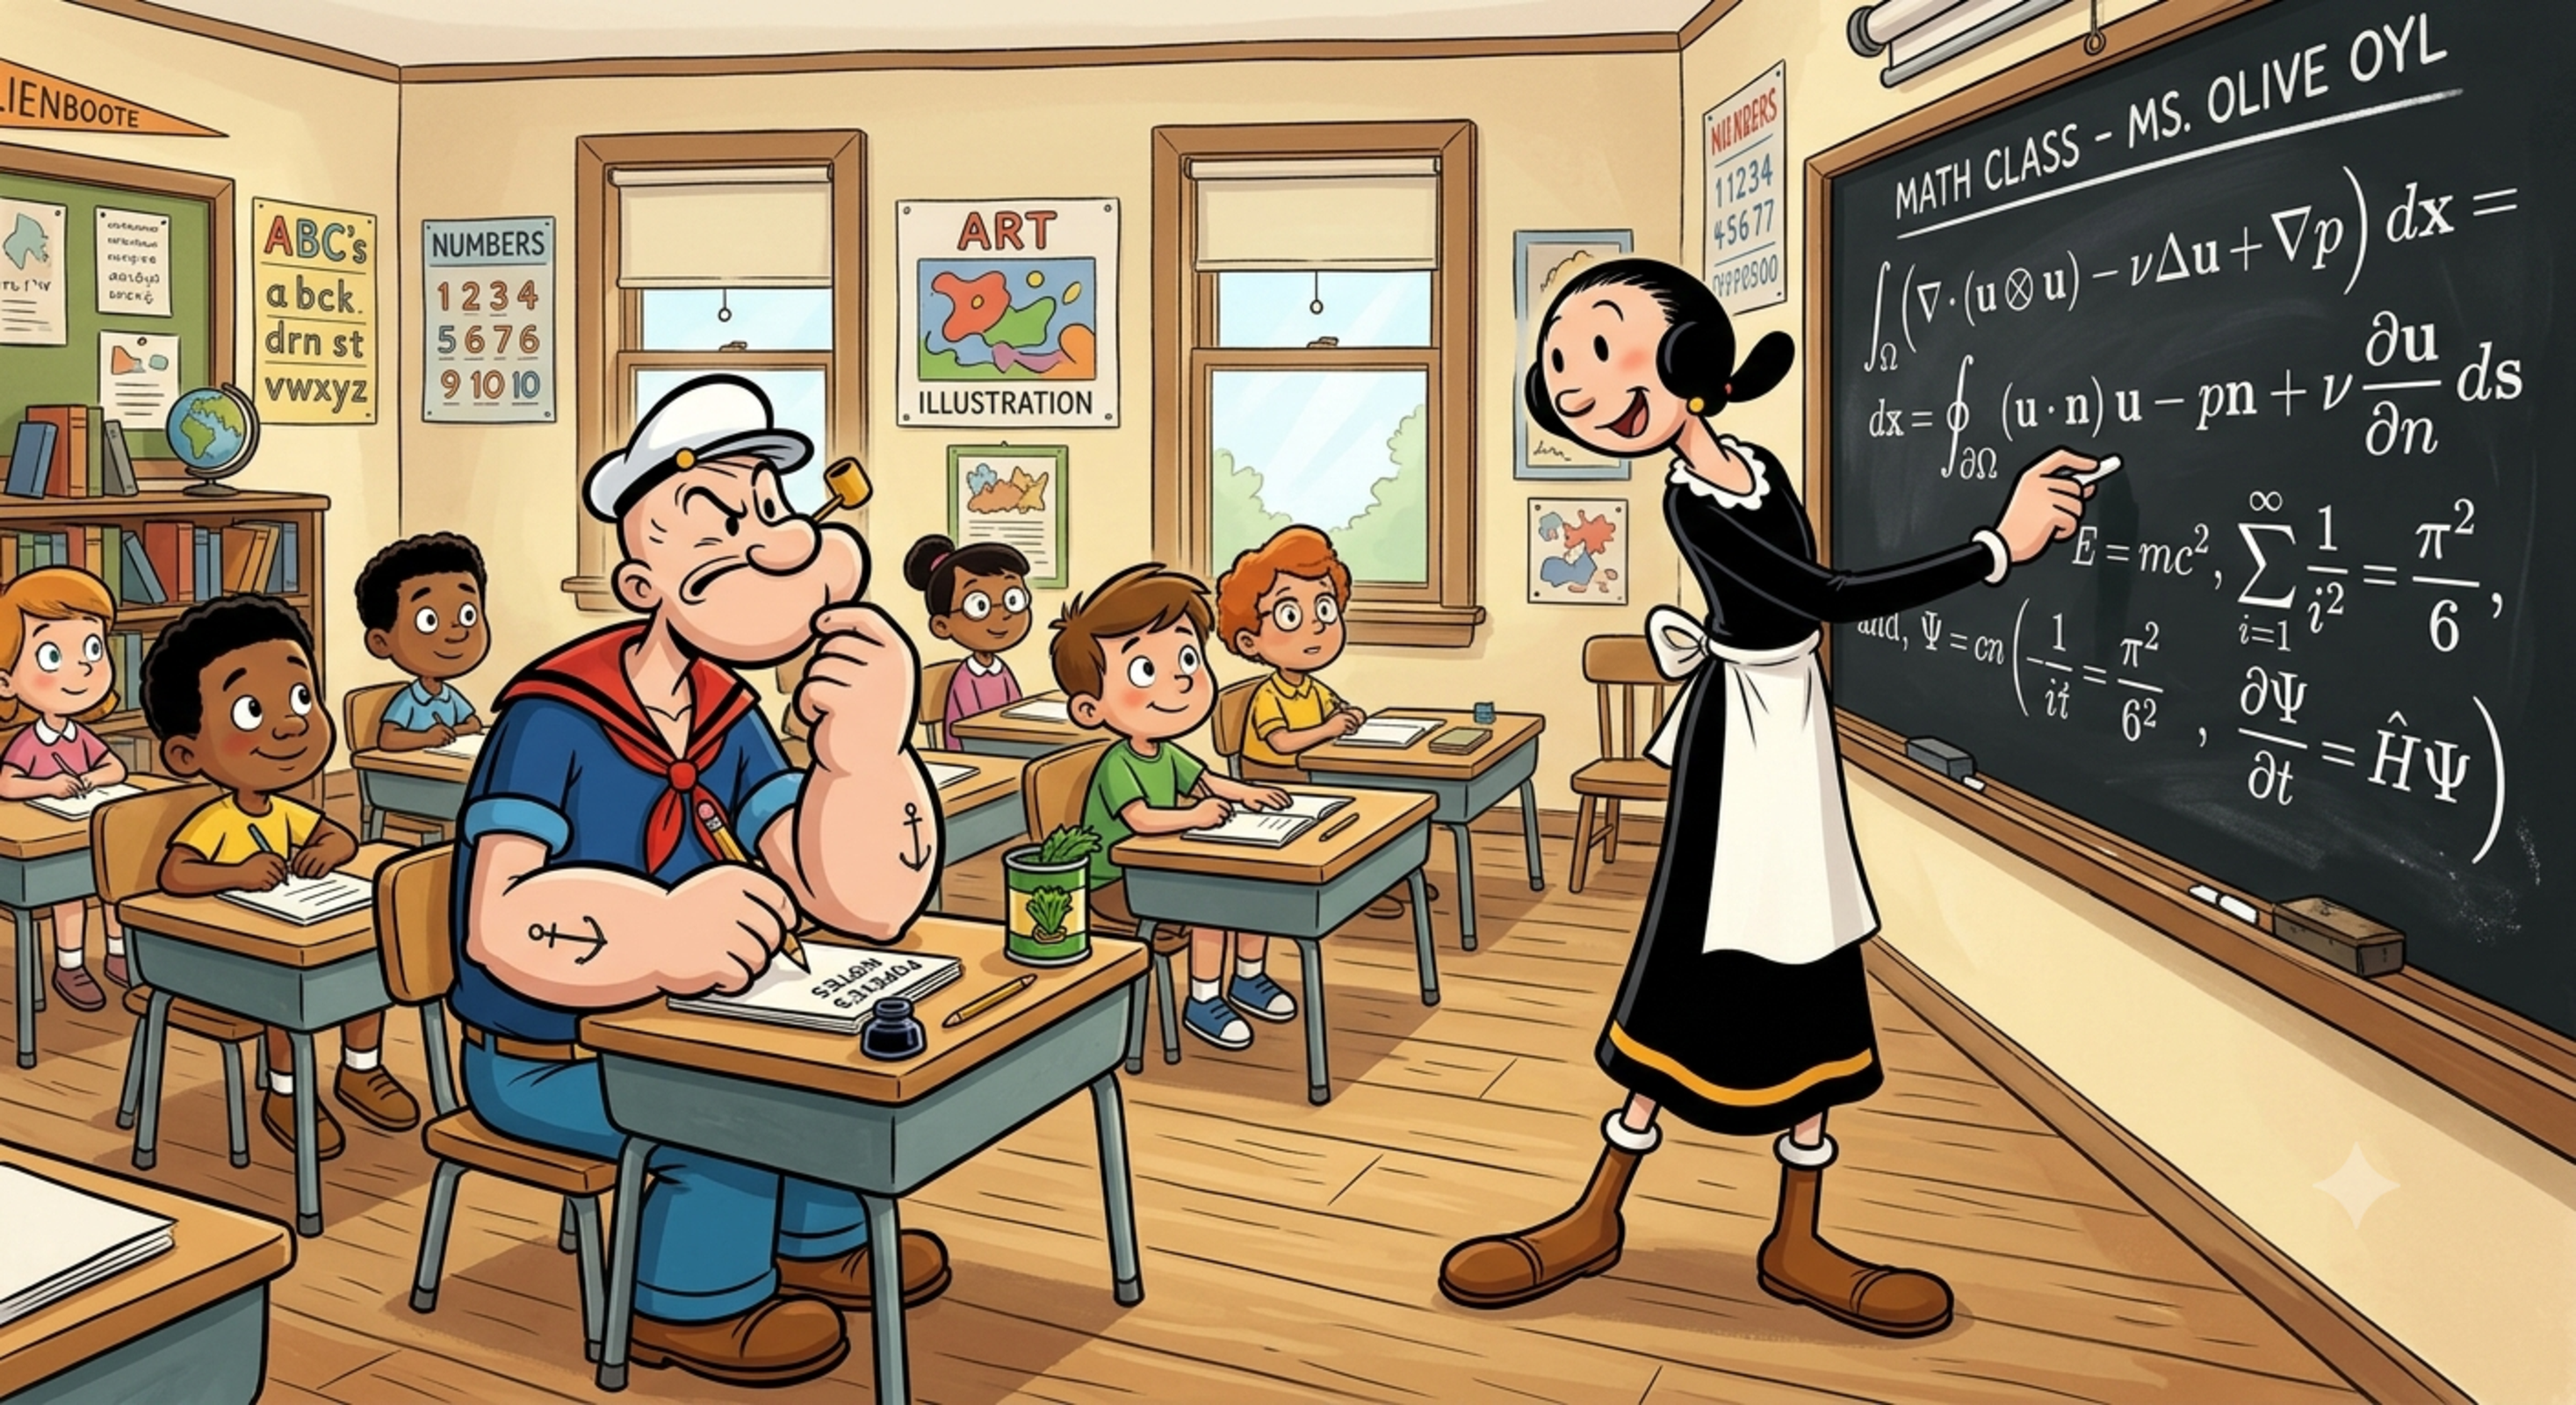
\includegraphics[width=\linewidth]{../img/actuals/popeye_maths.pdf}
\end{wrapfigure}

\begin{compactitem}
    \item Which notes (frequencies) are present
    \item How strong each note is
\end{compactitem}

It’s like having a machine that listens to a chord and says:

  “I hear a C note, an E note, and a G note.”

Underlying FFT is a mathematical process called the Fourier Transform which involves many laborious calculations. FFT is an algorithm that computes the same result much more efficiently. It does this by identifying redundancy in the actual steps taken and eliminating them without reducing the accuracy of the result. This means that the process can be completed in a manageable amount of time.

In the SONAR notes it is explained that the system can identify and estimate the speed of the object of interest. It does this by using the distinctive frequencies of the sound produced by FFT to compare against a database of known ships or submarines. This database has been built up over years by the various navies of the world and some of it is included in MNW. DEMON another tool available can take the output from the FFT and clean it up so that speed of the target can be estimated, This is also modelled in MNW. The types of sounds that can be detected include:

\begin{compactitem}
    \item Water flow arround the hull
    \item Engine (steam, turbine, diesel)
    \item Propeller noises
    \item Mechanical noises made by fans, generators etc.
    \item Human noises
    \item Many others
\end{compactitem}

So sadly, just like taxes, maths actually underpins everything. The good thing is you don't need to be an expert to use MACS successfully in game, but if you do want to know more Appendix B has more detail.
\pagebreak
\section{Appendix B - Technical Notes}
\label{sec:Appendix_B}
\subsection{Normalisation}

One of the principal challenges in SONAR processing is that the underwater acoustic environment is highly dynamic. Background noise levels vary due to sea state, vessel traffic, marine life, weather conditions, and the motion of the sonar platform itself. As a result, detection algorithms must distinguish meaningful targets from continually changing acoustic backgrounds. To reduce the impact of this MACS uses a statistical technique called normalization. MACS's normalisation is enabled with a toggle (Section 3) with configurable parameters in the settings panel.

\subsubsection{What MACS does}

\textbf{The Process:} raw acoustic information is fed from MNW into MACS which then applies a Fast Fourier Transform (FFT) to convert the data from the time domain to the frequency domain. Sliding-window z-scores can then be computed for each frequency bin or beam direction. Each FFT value is compared with its local neighbourhood and converted into a z-score that measures how many standard deviations it lies above or below the local background level. If a particular frequency band suddenly exhibits energy that is significantly higher than its recent average, the resulting z-score will be increased relatively. Such behaviour may indicate the presence of a target, such as a submarine, underwater vehicle, or marine mammal. It is the relative differences that are then colour mapped to the LOFAR display. The process is summarized in Figure 22.

\begin{figure}[ht]
	\centering
	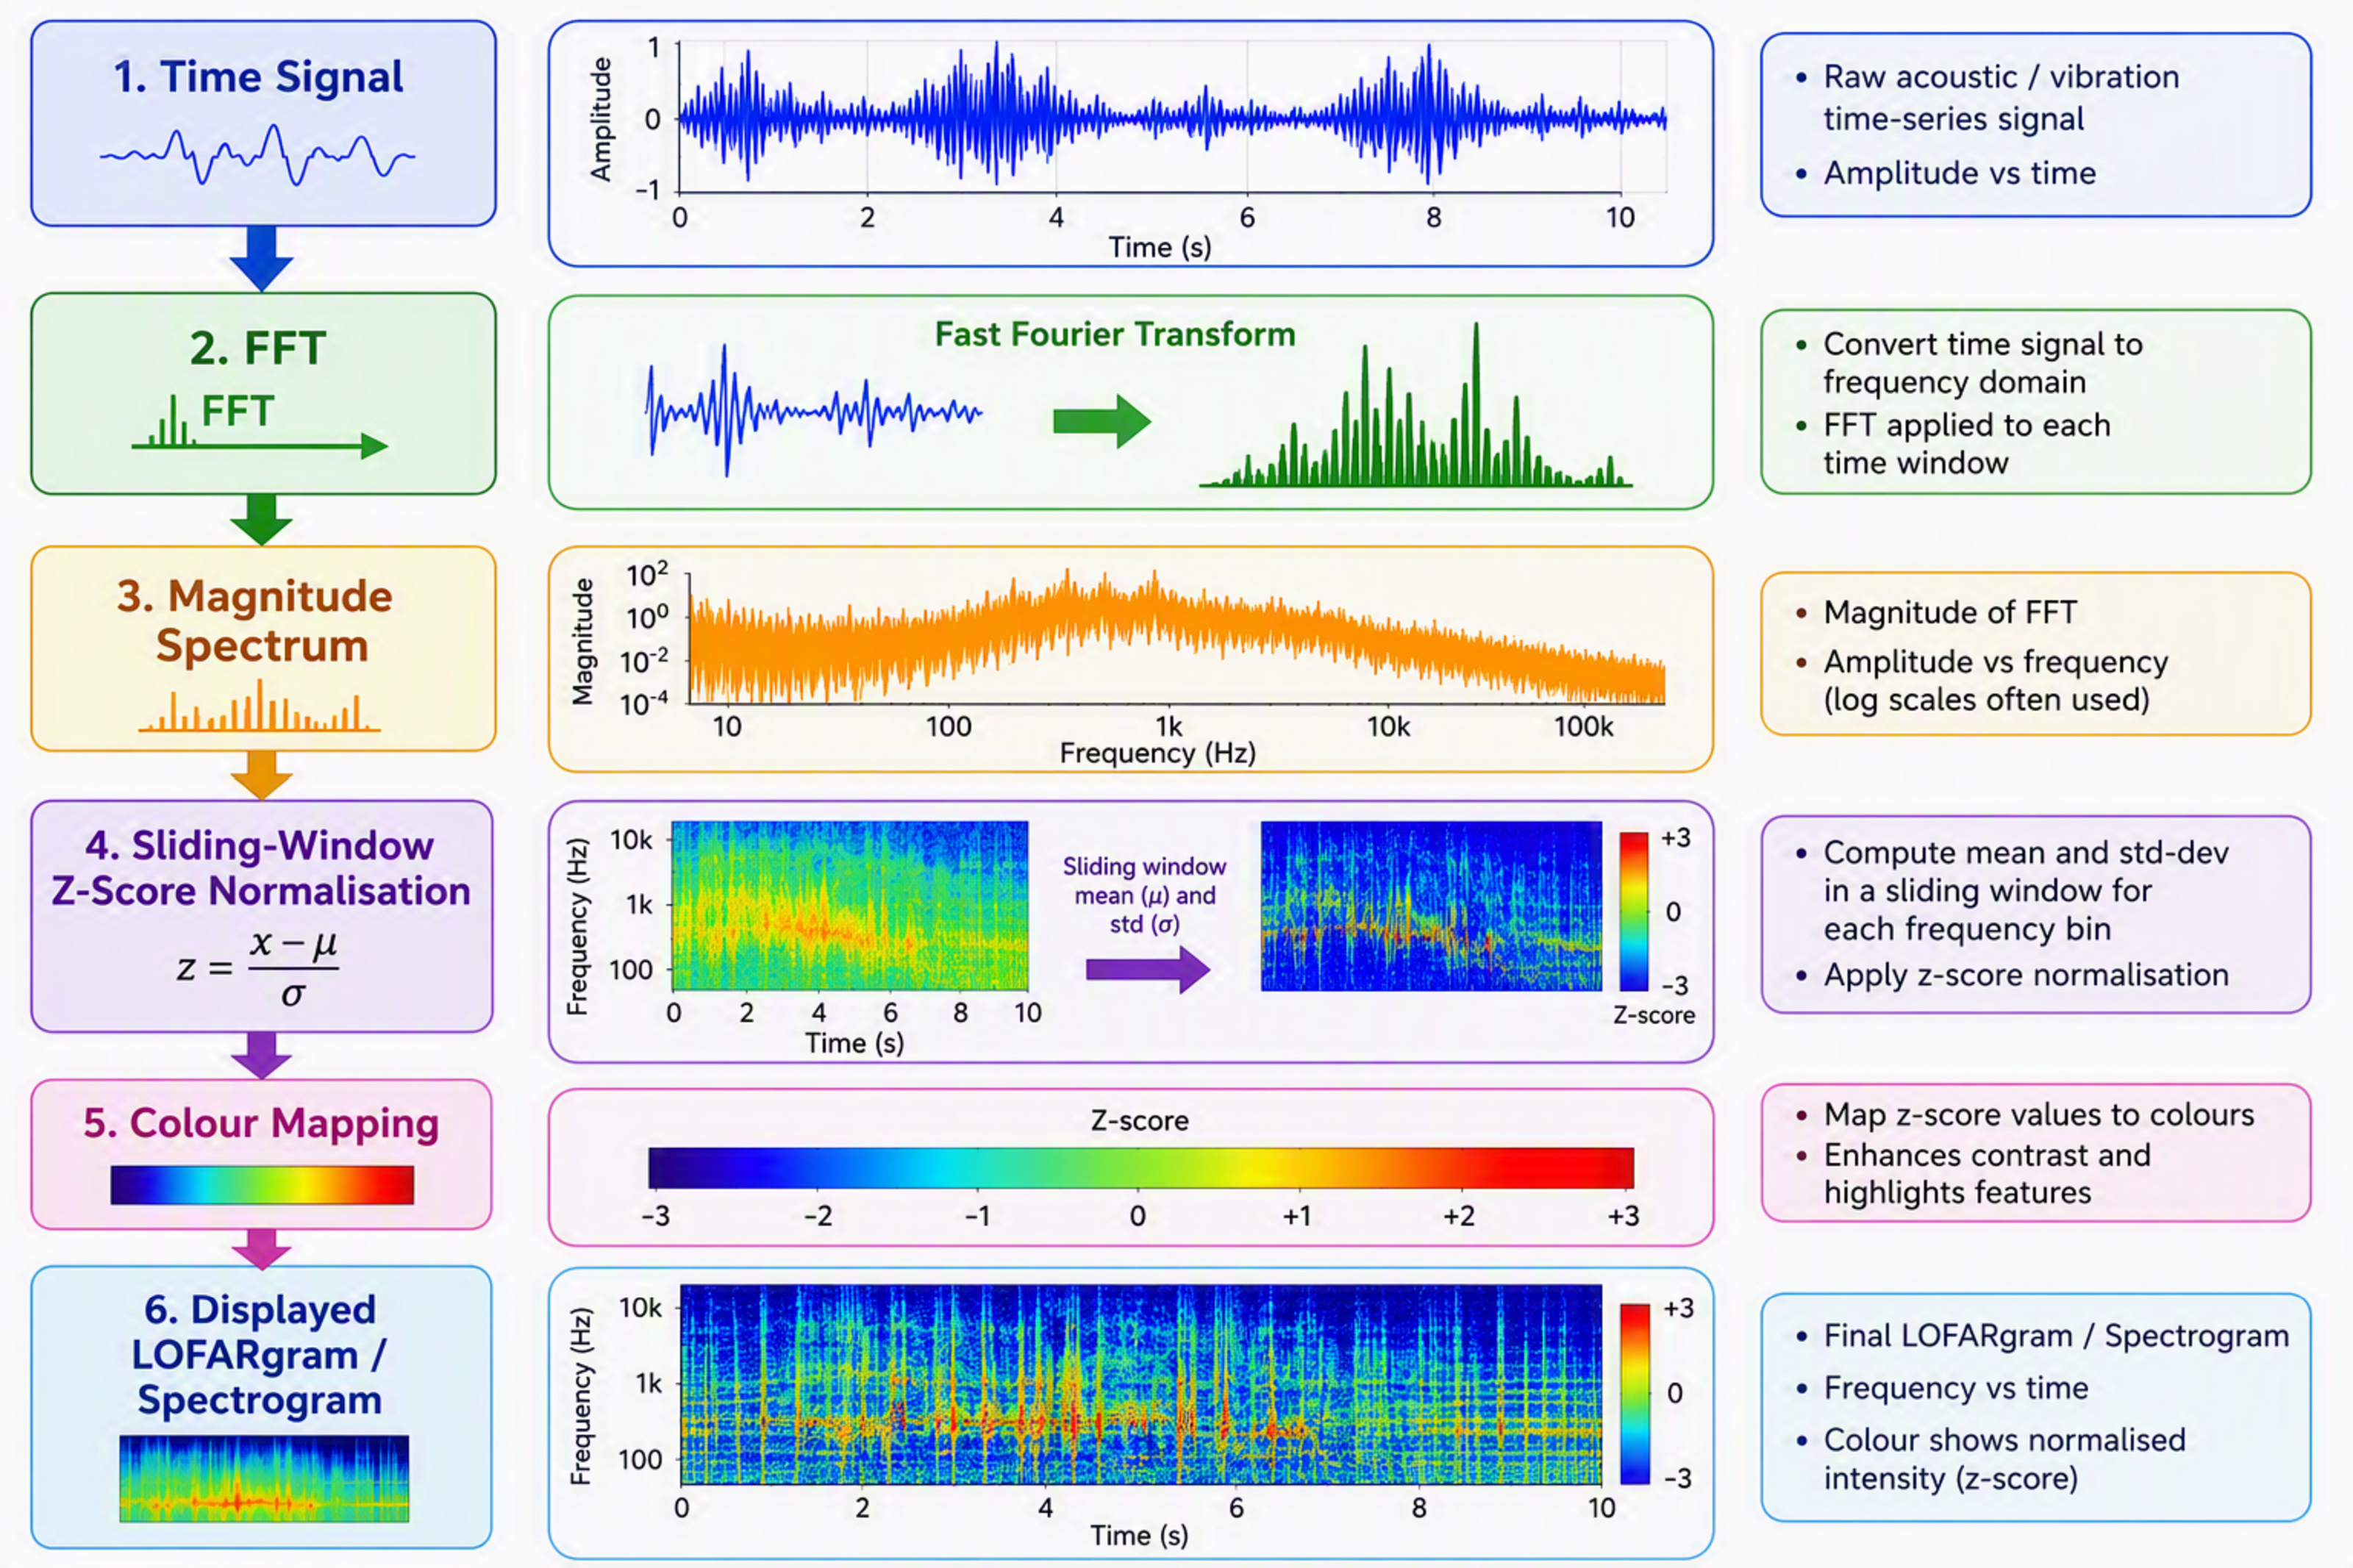
\includegraphics[width=400px]{../img/actuals/normalisation.pdf}
	\caption{FT from time domain to frequency domain}
\end{figure}


\textbf{Sliding window z-score:} is a statistical algorithm that measures how unusual a current observation is relative to recent observations (the window) rather than relative to the entire dataset. This means that the current observation is measured locally to its windowed set. The window slides along the data set as the analysis progresses. This adaptive normalisation continuously updates as new data arrive, allowing the detection process to remain sensitive even when the overall acoustic environment changes.

For a measured acoustic feature in each frequency bin the normaliser computes:

\[
z_{t} = \frac{x_{t} - \mu_{t}}{\sigma_{t}} \times \mathrm{Normalisation Output Scale}
\]

Where:
\begin{compactitem}
    \item $\mu_{t}$ is the mean computed over a recent time window (width controlled by Mean Half-Width see Parameters below).
    \item $\sigma_{t}$ is the standard deviation computed over across a potentially different sliding window (width controlled by Standard Deviation Half-Width see Parameters below).
    \item Normalisation Output Scale is a multiplier (range 1-50, default 20) that rescales z-scores into a range compatible with the Floor / Dynamic Range colour scale.
\end{compactitem}

% Both windows are computed efficiently using O(n) prefix sums -- no per-frame re-computation cost.

\subsubsection{MACS - LOFAR style example - from FFT to colour-mapping.}

The whole process is best explained with an simplified example. Given a set of raw FFT magnitudes, suppose one FFT frame contains these frequency bins:

 \begin{tabular}{ll}
    Frequency Hz & Magnitude \\
    \hline
    10 & 95 \\
    20 & 102 \\
    30 & 98 \\
    40 & 105 \\
    50 & 140 \\
    60 & 104 \\
    70 & 97 \\
    80 & 101\\
    90 & 99
 \end{tabular}

The 50 Hz bin (140) is suspected to be a machinery tone sitting above a background level of roughly 100. The question is, whether the difference between the tonal and background is significant. This is where MACS can assist by determining the significance and then visualise that.

Assume a window half-width of 2 bins which means the window always contains $2 \times 2 + 1 = 5$ bins (the centre value and two either side). For the first position the window is centred on Bin 3:

 \begin{tabular}{lllll}
    95 & 102 & 98 & 105 & 140 \\
    \hline
    1 & 2 & 3 & 4 & 5
 \end{tabular}

The algorithm calculates from those 5 values:
\begin{compactitem}
    \item Mean $\mu = 108$
    \item Standard deviation $\sigma = 16$
\end{compactitem}

Then it computes the z-score only for the centre bin (Bin 3).

\[
z_{3} = \frac{98 - 108}{16}
\]
\[
z_{3} = -0.63
\] 

Now the window slides right by one bin:

 \begin{tabular}{lllll}
    102 & 98 & 105 & 140 & 104 \\
    \hline
    2 & 3 & 4 & 5 & 6
 \end{tabular}

Now the centre is Bin 4. A completely new mean and standard deviation are calculated $\mu = 109.8$, $\sigma = 15.3$ resulting in $z_{4} = -0.31$
 
Window slides again

 \begin{tabular}{lllll}
    98 & 105 & 140 & 104 & 97 \\
    \hline
    3 & 4 & 5 & 6 & 7
 \end{tabular}

Now the centre is Bin 5, the machinery tone. $\mu = 108.8$, $\sigma = 15.9$ so $z_5 = 2.0$. The machinery line stands out because it is two standard deviations above the local background.

Continuing across the entire spectrum; the process repeats until every FFT bin has its own z-score.

 \begin{tabular}{llc}
    Bin & Magnitude & Z-Score \\
    \hline
    1 & 95 & -0.8\\
    2 & 102 & 0.1\\
    3 & 98 & -0.6\\
    4 & 105 & -0.3\\
    5 & 140 & 2.0\\
    6 & 104 & 0.1\\
    7 & 97 & -0.5\\
    8 & 101 & 0.0\\
    9 & 99 & -0.2
 \end{tabular}

Notice that the raw amplitudes have disappeared. Every bin is now expressed in terms of how unusual it is relative to its neighbours. The final step is mapping the z-scores to a colour map.

\begin{tabular}{ll}
    Z-Score & Colour \\
    \hline
    \verb|<| -1 & Dark Blue \\
    -1 to 0 & Blue \\
    0 to 1 & Green \\
    1 to 2 & Yellow \\
    2 to 3 & Orange \\
    \verb|>| 3 & Red
 \end{tabular}

This results in the following display where the 50 Hz machinery line now appears as a bright orange feature, distinct from the background.

 \begin{tabular}{lllcl}
    Bin & Frequency Hz & Magnitude & Z-Score & Color\\
    \hline
    1 & 10 & 95 & -0.8 & Blue\\
    2 & 20 & 102 & 0.1 & Green\\
    3 & 30 & 98 & -0.6 & Blue\\
    4 & 40 & 105 & -0.3 & Blue\\
    5 & 50 & 140 & 2.0 & Orange\\
    6 & 60 & 104 & 0.1 & Green\\
    7 & 70 & 97 & -0.5 & Blue\\
    8 & 80 & 101 & 0.0 & Blue\\
    9 & 90 & 99 & -0.2 & Blue
 \end{tabular}

Suppose another region of the spectrum looks like this:

\begin{tabular}{ll}
    Frequency Hz & Magnitude \\
    \hline
    500	& 20 \\
    510	& 21 \\
    520	& 20 \\
    530	& 26 \\
    540	& 19
\end{tabular}

The standout tone at 530 Hz is only 26 magnitude, which seems tiny compared with the 140 at 50 Hz but the local mean $\approx 21$ and the local standard deviation $\approx 2$ gives $z = \frac{26-21}{2} = 2.5$. This second tone gets a higher z-score than the 50 Hz one so in the final LOFARgram it may actually appear brighter, because it is more unusual relative to its local noise environment.

\begin{faintquote}
    That is the key idea behind the statement: "The algorithm used is a sliding-window z-score of the FFT magnitude output before colour mapping." The colours no longer represent absolute acoustic energy. They represent how significant each FFT bin is relative to its local background.
\end{faintquote}

Several example spreadsheets are provided for this process in the Spreadsheets folder at the \href{https://github.com/nbowling/MACS_Guide_Working}{GitHub repository} for this document.

\subsubsection{Adjustment Parameters via the Setting Panel}

MACS has sensible defaults for the key normalisation parameters however there are times when you would want to fine tune them. Turn on normalisation by ticking the option box on the LOFAR panel then clicking settings $\rightarrow$ Analysis Defaults tab. The normalisation settings are at the bottom of the panel.

\begin{compactenum}
    \item \textbf{Mean Width:} Sliding window half-width (in frames) used to compute the local mean. Wider $\rightarrow$ slower adaptation to changing noise level.
    \item \textbf{StdDev Width:} Sliding window half-width for standard deviation. Can differ from Mean Width. If $\sigma > 2  \times \mu$, the noise floor is highly non-stationary.
    \item \textbf{Output Scale:} Multiplies all z-scores before colour mapping. Increase if the waterfall is too dim, decrease if it saturates. Start around 20 and adjust by eye.
\end{compactenum}

It is difficult to give exact advice for the best settings because they are very situation dependent, in general:

\begin{compactenum}
    \item Short mean window $\rightarrow$ remove local background variations and slow trends.
	\item Long standard-deviation window $\rightarrow$ estimate the ambient noise floor robustly.
\end{compactenum}

This tends to make narrowband machinery tones and transient features more visible without allowing them to significantly affect the variance estimate.

As a general rule of thumb the following table gives basic usage:

\begin{tabular}{ll}
    Window size	& Effect \\
    \hline
    Very small & Highly adaptive, noisy normalisation \\
    Moderate & Good compromise \\
    Very large & Stable statistics, less adaptive \\
    Mean window \verb|<| Std-dev window & Common and often desirable \\
    Mean window $\approx$ Std-dev window & Standard sliding z-score \\
    Std-dev window too small & Can suppress strong events
\end{tabular}

A useful way to think about it is:
\begin{compactitem}
	\item Mean window controls how quickly the baseline can move.
	\item Std-dev window controls what the algorithm considers to be the "normal" noise level.
\end{compactitem}

For LOFAR or spectrogram preprocessing, the standard-deviation window is often chosen several times larger than the mean window so that transient or tonal features remain prominent after normalisation.

\begin{faintquote}
    Consider a passive SONAR system monitoring vessel noise. The background acoustic level may gradually increase as ocean conditions change during the day. A conventional threshold based on absolute signal level might generate numerous false alarms or miss weak targets. In contrast, a sliding-window z-score compares the current observation with the local acoustic environment. A ship propeller tone that rises above the recent background will produce a large positive z-score, making it easier to detect even when absolute noise levels are elevated. This adaptive normalisation continuously updates as new data arrive, allowing the detection process to remain sensitive even when the overall acoustic environment changes.

    \begin{compactenum}
        \item \textbf{Suppresses slowly varying broadband noise:} bins that are consistently loud have a high mean, which gets subtracted. What remains is deviations from the local average.
        \item \textbf{Enhances tonal lines:} a persistent narrowband tone will have a value consistently above its local mean, showing up as a bright persistent line even against a noisy background.
        \item \textbf{The z-score can go negative} (a bin quieter than average). The Floor control clips these to the background colour.
    \end{compactenum}
\end{faintquote}

\subsubsection{When to use}

Enable normalisation when the background noise level is high and tonal lines are hard to see. It is particularly effective when the ship is manoeuvring and the broadband level is changing; the local mean tracks the change and removes it. Disable it for clean recordings where tonals are already visible, or when you need absolute amplitude information for noise reference subtraction.
\begin{faintquote}
    In summary. Sliding-window z-score normalisation converts raw SONAR measurements into a measure of statistical deviation from the recent acoustic background, enabling robust target detection in noisy underwater environments.
\end{faintquote}

\subsection{Fourier Transform}
\subsubsection{Introduction}

Many things that vary over time or space appear complicated when viewed directly: a piece of music, a seismic tremor, a photograph, a radio transmission, or even fluctuations in financial data. The Fourier Transform (FT) offers a markedly different perspective. Instead of asking, “What is this signal doing at each moment?” it asks, “Which frequencies combine to create it?”

Named after the French mathematician Joseph Fourier (1768-1830), the transform originated from his work on heat conduction. Today it is one of the most important mathematical tools in science and engineering, fundamental to fields ranging from physics and telecommunications to medical imaging and machine learning. At its core, it is a mathematical microscope that peers into complex, messy signals and extracts the fundamental building blocks: pure frequencies. Whether studying sound waves, radar signals, vibration measurements, electrical systems, or digital communications, the FT provides a powerful way to understand how energy is distributed across different frequencies.

\subsubsection{From waves to ingredients an analogy: Unmixing the Smoothie}

An often used analogy for FT is to imagine making a fruit smoothie. Once blended, you have a single, uniform liquid. If someone asked you to measure the exact amount of strawberries, bananas, and milk in that finished glass, it would be almost impossible just by looking at it.

Two terms that commonly appear are \enquote{Time Domain} and \enquote{Frequency Domain}. Using our smoothie they can be explained in the following way:

\begin{compactitem}
    \item The Time Domain is the smoothie itself — the raw, combined signal as it exists in the real world over time.
    \item The Fourier Transform is the magic machine that takes the finished smoothie and separates it back into individual piles of fruit.
    \item The Frequency Domain is the recipe — the broken-down smoothie showing exactly how much of each ingredient (frequency) makes up the whole (Figure 23).
\end{compactitem}

\begin{figure}[ht]
	\centering
	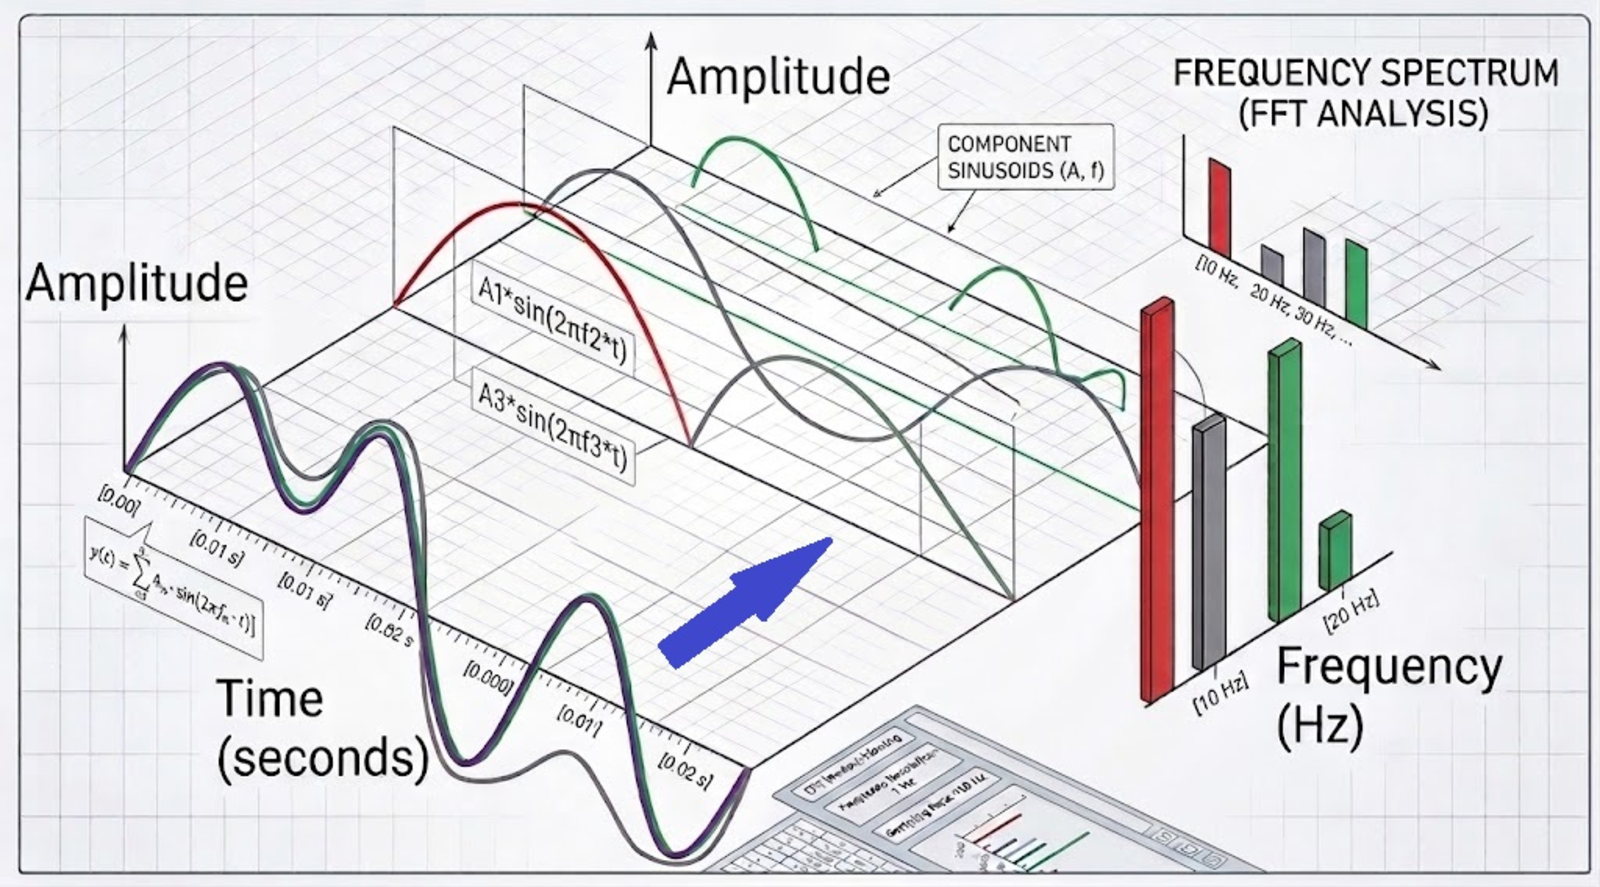
\includegraphics[width=300px]{../img/actuals/TD2FD.pdf}
	\caption{FT from time domain to frequency domain}
\end{figure}

\begin{faintquote}
    A signal can be represented in two complementary ways:
    \begin{compactitem}
        \item The time domain shows how it changes over time.
        \item The frequency domain shows the strength of its component frequencies.
    \end{compactitem}
\end{faintquote}

\subsubsection{Why is it relevant to me}

In underwater acoustic analysis, passive sonar techniques used by submarines and surface ships to detect, classify, and track underwater targets (like submarines, surface vessels, or torpedoes) rely on the FT, it is the core mathematical engine that makes LOFAR, DEMON and other sonar processing tools work. Undersea targets produce a complex mix of continuous broadband noise (water displacement, turbulent flow) and discrete narrowband tonal signals (machinery, engine vibrations, propeller blade passage). The FT isolates these hidden narrowband tonals from background ocean noise.

\begin{compactitem}
    \item Short-Time Fourier Transform (STFT): Hydrophones continually record continuous time-domain voltage/acoustic signals $f(t)$. Because underwater sound changes over time, the signal is chopped into overlapping time windows (slices), and an FT is computed for each window.
    \item Creating the "Lofargram" (Waterfall Display): The magnitude of each FT frame becomes a single row of pixels, where the x-axis represents Frequency, colour/brightness represents Signal Energy (dB), and the Y-axis scrolls downward representing Time.
\end{compactitem}


Key Applications of FT in LOFAR Analysis

\begin{compactenum}
    \item Target Classification and Fingerprinting:
    \begin{compactitem}
        \item Rotating propellers, reduction gears, onboard generators, and cooling pumps vibrate at precise frequencies.
        \item The FT isolates these frequencies as sharp vertical lines (tonals) on the Lofargram. Sonar operators match these line patterns against acoustic libraries to identify the exact class or ship name of a vessel miles away.
    \end{compactitem}
    \item Measuring Shaft/Blade RPM:
    \begin{compactitem}
        \item Propeller cavitation produces fundamental frequencies and harmonics. By applying the Fourier Transform, operators can calculate propeller blade counts and shaft rotation speeds (RPM) to determine target speed.
    \end{compactitem}
    \item Enhancing Signal-to-Noise Ratio (SNR):
    \begin{compactitem}
        \item Ocean background noise spreads across a wide band of frequencies. By running long FFT integration times (narrow frequency bins), the power of a single steady mechanical tone concentrates into a single frequency bin, making faint targets stand out clearly above the background noise.
    \end{compactitem}
\end{compactenum}


\subsubsection{The Basic Idea and Mathematical Definition}

Arguably, the FT is one of the most elegant and practical mathematical concepts ever devised although much credit must go to Euler who's insight was the starting point for Fourier.

The basic premise is that any periodic signal can be represented as a sum of sine and cosine waves of different frequencies, amplitudes, and phases.

\begin{compactitem}
    \item Frequency: How fast the wave repeats itself, measured as the number of complete cycles per second (Hertz, or Hz). Higher frequency means more rapid oscillations (e.g., a higher pitch in sound or higher speed in rotation).
    \item Amplitude: The height or strength of the wave, measured as the distance from its rest position to its highest peak. Higher amplitude means greater power or intensity (e.g., a louder sound or a higher peak voltage).
    \item Phase: The timing or relative position of a wave within its cycle at a specific starting point, measured in degrees ($0^\circ$  to $360^\circ$) or radians (0 to $2\pi$). If two waves are "in phase," their peaks align at the same time; if they are "out of phase," one is shifted horizontally relative to the other.
\end{compactitem}

For example, a square wave can be approximated by:
\[
    x(t)=sin(\omega t) + \frac{1}{3} sin(3\omega t) + \frac{1}{5}sin(5\omega t) + ...
\]
The symbol $\omega$ represents angular frequency and is closely related to ordinary frequency $f$, measured in cycles per second or Hertz (Hz)
\[
    \omega=2\pi f
\]
Where:
\[
\begin{aligned}
    \omega &= \text{angular frequency (radians per second)}  \\
    f &= \text{frequency (Hz)} \\
    2\pi &= \text{radians in one complete cycle}
\end{aligned}
\]

Although the square wave looks totally different from a sine wave, it can be constructed by adding together many sinusoidal components. The FT generalizes this concept to arbitrary signals.

For a continuous-time signal the Fourier Transform is defined as:
\[
    \hat{f}(\xi)=\int\limits_{-\infty}^\infty f (t) e^{-j2\pi \xi t}\,dt
\]
The inverse Fourier Transform reconstructs the original signal:
\[
    f(t)=\int\limits_{-\infty}^\infty X (\xi) e^{j2\pi \xi t}\,dt
\]

These equations show that the time and frequency domains contain equivalent information.

Where:
\begin{align*}
    f(t) &\quad\text{--}\quad \parbox[t]{12cm}{\raggedright \textbf{The Input Signal:} The original time-domain signal (e.g., sound pressure over time or a changing voltage).} \\[1.5ex]
    \xi &\quad\text{--}\quad \parbox[t]{12cm}{\raggedright \textbf{The Target Frequency:} The specific probe frequency being tested. The equation evaluates one value of $\xi$ at a time.} \\[1.5ex]
    e^{-j2\pi \xi t} &\quad\text{--}\quad \parbox[t]{12cm}{\raggedright \textbf{The Complex Rotator:} By Euler's identity ($e^{jx}=\cos x + j \sin x$), this term represents a point rotating around a unit circle in the complex plane at frequency $\xi$. The negative sign causes clockwise rotation.} \\[1.5ex]
    f(t)\cdot e^{-j2\pi \xi t} &\quad\text{--}\quad \parbox[t]{12cm}{\raggedright \textbf{The Signal Winding:} Multiplying the original signal $f(t)$ by this rotating complex exponential wraps the 1D signal into a 2D spiral in the complex plane.} \\[0.75ex]
    \int\limits_{-\infty}^{\infty} &\quad\text{--}\quad \parbox[t]{12cm}{\raggedright \textbf{Finding the Center of Mass:} Integrating sums up all the points on that spiral over all time.}
\end{align*}

\textbf{The Mechanical Intuition: "Winding" the Signal}

To visualize how the integration extracts a frequency, imagine wrapping a physical audio signal line around a circle at a variable winding rate:
\begin{compactenum}
    \item Unmatched Frequency ($\xi \ne$ signal frequency): The spiral winds unevenly. Points spread evenly around the center in all directions, causing positive and negative values to cancel out. The integral evaluates to roughly zero.
    \item Matched Frequency ($\xi =$ signal frequency): The signal's peaks line up on one side of the circle, pulling the entire spiral off-center. The integral sums these aligned values, resulting in a large spike.
\end{compactenum}

The final output, $\hat{f}(\xi)$, is a complex number where the magnitude represents the strength of that frequency in the signal, and the angle (phase) indicates how that frequency aligns in time. While magnitude often receives the most attention, phase is essential for accurately reconstructing the original waveform.

Suppose a signal contains:
\[
    x(t) = 3 \sin( 2 \pi 50 t) + 2 \sin(2 \pi 120 t) \quad \text{(Figure 24)}
\]

 \begin{figure}[ht]
	\centering
	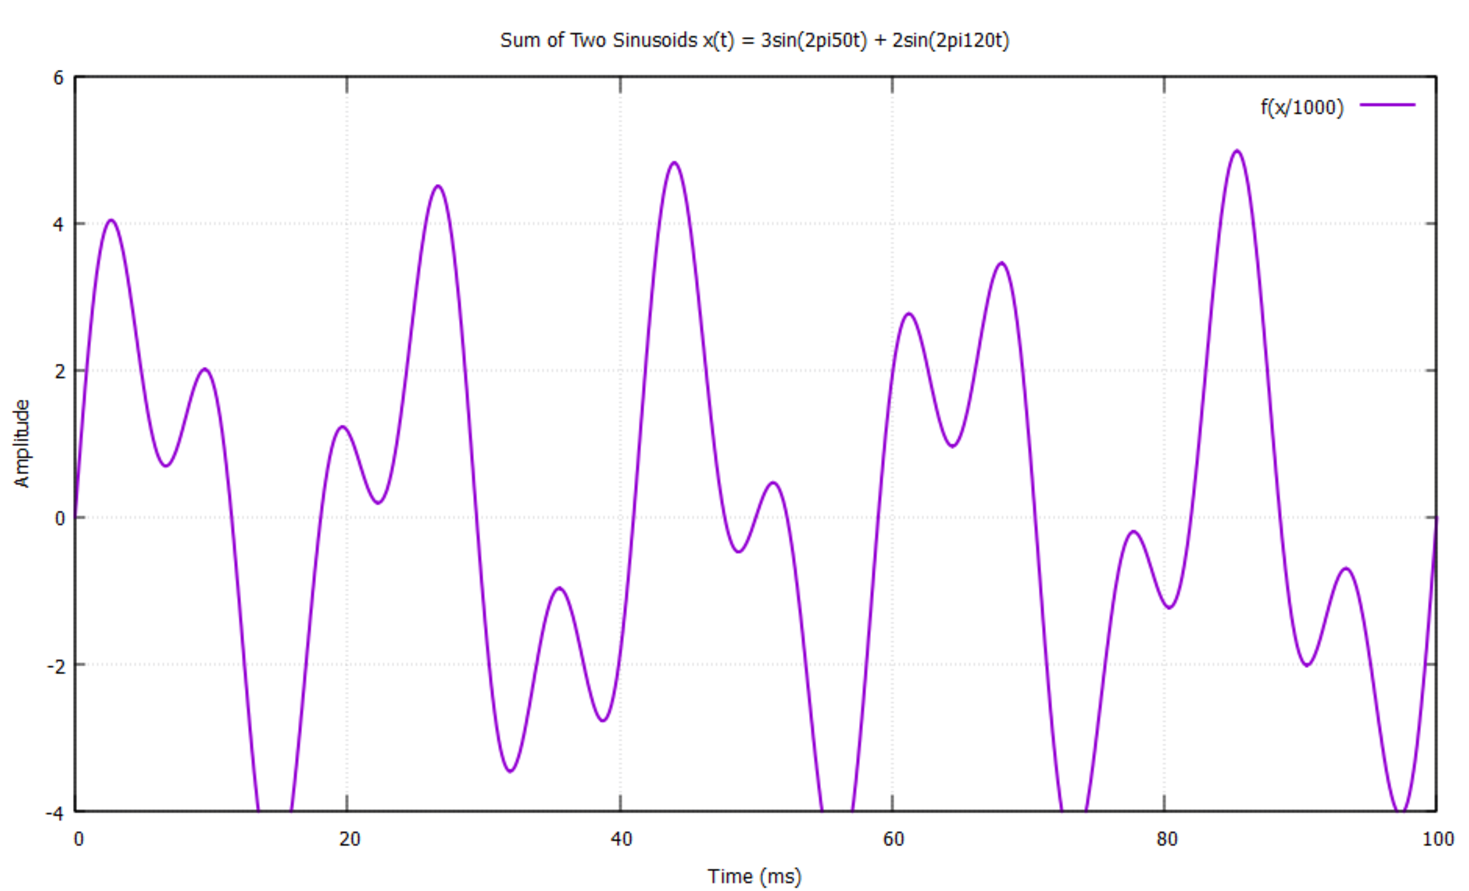
\includegraphics[width=300px]{../img/actuals/CmplxWave.pdf}
	\caption{Complex wave function}
\end{figure}

Visually, the waveform is complicated, but after applying the FT, two clear peaks appear; the transform immediately reveals the signal's composition.

 \begin{tabular}{lc}
    Frequency & Amplitude \\
    \hline
    50 Hz & 3 \\
    120 Hz & 2
 \end{tabular}

\subsubsection{Discrete Fourier Transform (DFT) and Fast Fourier Transform (FFT)}
Real-world measurements are sampled digitally. Consequently, computers use the Discrete Fourier Transform (DFT) rather than the continuous FT. The DFT converts sampled data into discrete frequency bins.

For a sequence containing N samples:
\[
 X[k]=\sum_{n=0}^{N-1}x [n] e^{-j2\pi kn/N}
\]
However the DFT can be computationally expensive for large datasets.  Instead modern analysts use the FFT algorithm to compute the DFT. The FFT is most commonly associated with James Cooley and John Tukey, who published the famous Cooley-Tukey FFT algorithm in 1965. Their paper showed how to compute a Discrete Fourier Transform much more efficiently, reducing the computational effort from roughly $O(N^2)$ operations to $O(N\log_{10} N)$. For a million-sample signal, the FFT may perform thousands of times faster than a direct DFT calculation.

\subsubsection{In terms of Marine Acoustics: A Concrete Audio Example}

In underwater passive sonar, a classic task is calculating the Blade Pass Frequency (BPF) of a submarine's propeller using a LOFARgram (direct spectrum analysis) and a DEMON spectrum (demodulation envelope analysis). Below is a complete numerical example demonstrating how a sonar signal processor converts raw acoustic line frequencies into target speed and machinery specifications.

\textbf{Scenario \& Given Data}

A passive sonar hydrophone array detects a contact. The signal processing pipeline in MACS generates two spectral plots from the sound recording:

\begin{compactenum}
    \item LOFAR Spectrum: Displays a strong, fundamental machinery tonal line at $f_{tonal} = 120 Hz$.
    \item DEMON Spectrum: Displays an envelope modulation spectrum with distinct harmonic peaks at 5 Hz, 10 Hz, 15 Hz, and 20 Hz".
\end{compactenum}

From intelligence database records, this target class is known to use a 7-bladed propeller ($N_{blades} = 7$) with a pitch (P) of 8 feet per revolution and a known slip (S) of 15\verb|%| (Efficiency Factor = $1 - 0.15 = 0.85$).

\textbf{Step-by-Step Numerical Analysis}
\begin{compactenum}
    \item \textbf{Determine the Fundamental Shaft Frequency (SR):}
        \begin{compactenum}[i]
            \item In the DEMON spectrum, the periodic mechanical modulation of propeller cavitation produces peaks at fundamental rotation rates and their harmonics.
            \item The lowest fundamental peak in the envelope spectrum represents the Shaft Fundamental (SF).
            \item $SF = 5$ Hz
        \end{compactenum}
    \item \textbf{Calculate Propeller Shaft Speed (SR in RPM):}
        \begin{compactenum}[i]
            \item To convert the shaft fundamental from Hertz (revolutions per second) to Shaft Rate (SR) in Revolutions Per Minute (RPM)
            \item $SR = SF \times 60$ $\rightarrow$  $5 \times 60 = 300$ RPM
        \end{compactenum}
    \item \textbf{Calculate the Blade Rate (BR):}
        \begin{compactenum}[i]
            \item The Blade Pass Frequency is the rate at which individual propeller blades pass a fixed point. It is the product of the shaft frequency and the number of blades
            \item $BPF=SF \times N_{blades} \rightarrow 5 \times 7 = 35$ Hz
            \item On a LOFARgram or DEMON spectrum, a peak would appear right at 35 Hz
        \end{compactenum}
    \item \textbf{Identify Machinery Gear Ratio from LOFAR Tonal:}
        \begin{compactenum}[i]
            \item Now we link the DEMON results back to the LOFAR spectrum tonal line ($f_{tonal} = 120$ Hz).
            \item If this tonal line is generated by a diesel engine or reduction gear driving the main shaft, we can calculate the exact gear/vibration ratio (R) relative to the shaft turn
            \item $R = \frac{f_{tonal}}{SF} \rightarrow \frac{120}{5} = 24$
            \item This tells the sonar analyst that the machinery generating the 120 Hz tone turns at 24 times the rate of the main propeller shaft ($24 \times 300 = 7,200 RPM$).
        \end{compactenum}
\end{compactenum}

\textbf{Theoretical Speed} if no propeller slip.

\begin{compactenum}
    \item Distance per minute = $SR \times P$ = $300 \times 8 = 2,400$ ft/min
    \item Distance per hour = $2,400 \times 60$ = 144,000 ft/hr $\rightarrow$ $\frac{144,000}{6076} \approx$ \underline{23.7 Knots/hr} (6076 ft/nautical mile)
\end{compactenum}

\textbf{Speed accounting for propeller slip}

\begin{compactenum}
    \item $\text{Theoretical Speed} \times (1 - S)$
    \item $23.7 \times (1 - 0.15) = 23.7 \times 0.85 \approx$ \underline{20.1 Knots / hr}
\end{compactenum}

Both steps can be combined in one formula:

\[
    \text{Speed (Knots)} = \frac{SR \times P \times ( 1 - S)}{6076}
\]

\textbf{Summary of Results}

\begin{tabular}{lll}
    Parameter & Formula & Calculated Value \\
    \hline
    Shaft Frequency (SF) & Primary DEMON peak & 5.0 Hz \\
    Shaft Rate & $SF \times 60$ & 300 RPM \\
    Blade Pass Frequency (BPF)	& $SF \times N_{blades}$ & 35 Hz \\
    Machinery Gear Ratio & $f_{tonal}/SF$ & 24:1 \\
    Speed through water & $\text{Speed (Knots)} = \frac{SR \times P \times (1 - S)}{6076}$ & 20.1 Kts/hr
\end{tabular}

By performing these steps, a passive sonar operator confirms not only the target's operating speed, but also verifies the contact's identity against known propeller and engine drive signatures.

\subsubsection{Limitations}
A standard Fourier Transform tells us which frequencies exist in a signal, but not always when they occur. If a song changes from a bass note to a violin note, the overall transform identifies both frequencies but does not precisely mark their timing.

These limitations are the reason other techniques such as the Short-Time Fourier Transform, spectrograms, wavelets, and order tracking were developed. For many marine acoustic problems, a spectrogram (successive FFTs over time) is often more informative than a single Fourier Transform because it reveals how shaft-rate, blade-pass, and cavitation frequencies evolve as vessel speed changes.

There is also a fundamental trade-off: greater precision in time generally comes at the cost of precision in frequency, and vice versa. This relationship is closely related to the uncertainty principle in physics.

\subsubsection{Conclusion}
The Fourier Transform is a cornerstone of modern science and engineering. By converting signals from the time domain to the frequency domain, it reveals information that is often hidden in raw measurements. Its digital implementation through the Discrete Fourier Transform and Fast Fourier Transform enables practical analysis of everything from music and radio transmissions to vibration measurements and underwater acoustics. As a result, the Fourier Transform remains one of the most widely used mathematical techniques for understanding, analysing, and processing complex signals.

\subsection{LOFAR}
\textcolor{commentGreen}{*** WIP ***}

What it is: A standard acoustic spectrogram displayed as a waterfall. Each new FFT frame is added as a horizontal line of pixels scrolling bottom to top; the horizontal axis is frequency; colour encodes amplitude in dB. Persistent vertical lines marching across the display indicate tonal components — discrete narrowband signals that stand out from the broadband noise background.

\textbf{Signal path:}

\begin{compactenum}
    \item Audio samples arrive from the engine (live or file playback).
    \item An optional bandpass filter is applied.
    \item An optional noise reference is subtracted.
    \item Samples are accumulated in an overlap buffer.
    \item An FFT is computed with zero-padding to match the display pixel width.
    \item Magnitudes are converted to dB.
    \item Optional normalisation is applied.
    \item The result is mapped through the Floor / Dynamic Range colour scale and painted as one column.
\end{compactenum}

\textbf{Key parameters:} FFT Size, Overlap, Floor, Dynamic Range, Normalisation, $F_{min}$ / $F_{max}$ display limits.

\subsection{DEMON}
\textcolor{commentGreen}{*** WIP ***}

\textbf{What it is:} DEMON (Detection of Envelope Modulation ON Noise) extracts the low-frequency modulation imposed on broadband acoustic noise by a vessel's rotating machinery (primarily propeller shaft and blade-rate harmonics). The result is a second spectrogram whose frequency axis covers 0 - $F_{max}$ Hz (typically 0 - 50 Hz), revealing shaft rotation rates and blade rates that are far too low to appear in the LOFARgram.

\textbf{Signal path:}

\begin{compactenum}
    \item Samples are bandpass-filtered to the selected DEMON band.
    \item The amplitude envelope is extracted using a 63-tap Type III linear-phase Hilbert FIR filter (Hann-windowed). This produces a clean, phase-correct envelope signal without the DC bias of simple rectification.
    \item The envelope is decimated by a factor computed as $\max(\frac{Fs}{(2 \times F_{max-demon})}, 1)$, floored by Nyquist and ceilinged by FFT resolution requirements. This dynamically sets the decimated sample rate just high enough to represent the DEMON band without wasting computation.
    \item An FFT is computed on the decimated envelope using the DEMON FFT size and overlap.
    \item The result is displayed as a waterfall, with the same Floor / Dynamic Range colour scale.
\end{compactenum}

 \begin{figure}[ht]
	\centering
	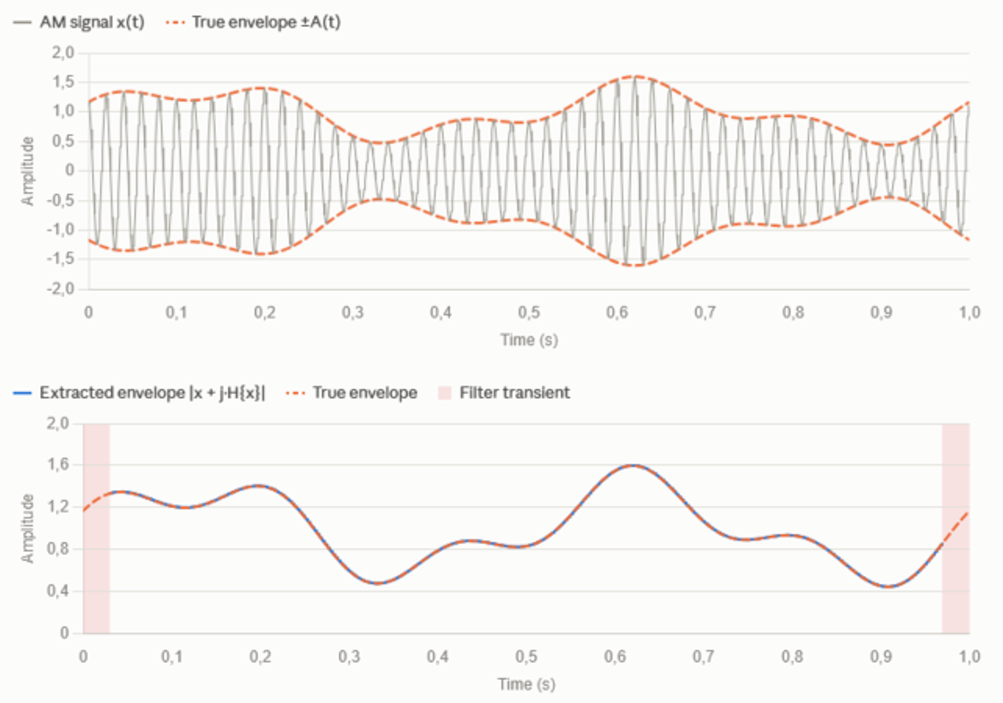
\includegraphics[width=300px]{../img/actuals/DEMONchart.pdf}
	\caption{DEMON process}
\end{figure}

\textbf{Why this works:} Rotating machinery amplitude-modulates the broadband acoustic noise it generates. For propeller-driven vessels, propeller blades periodically interrupt the cavitation noise; for diesel-engined vessels, piston firing events modulate the radiated noise at crankshaft rate and its harmonics. DEMON demodulates this carrier to make those low frequencies directly visible. It is effective for both propeller shaft / blade-rate detection (surface ships, submarines underway) and diesel engine firing rate detection (diesel-electric submarines at low speed).



\textbf{Key parameters:} DEMON band sets the acoustic carrier band to demodulate, DEMON Display Max ($F_{max}$ of the DEMON output display axis), DEMON FFT Size, Overlap, Floor, Dynamic Range.

\subsection{Cepstrum}
\textcolor{commentGreen}{*** WIP ***}

\textbf{What it is:} The real cepstrum is computed as:

\[
C(\tau) = \mathrm{IFFT}\{\log |X(f)|\}
\]

where X(f) is the FFT of the input signal and the log is of the \textbf{linear magnitude} (not dB - log is applied once inside the cepstrum formula). The result is plotted with the horizontal axis in quefrency (milliseconds), which is the reciprocal-domain equivalent of frequency.

A peak at quefrency $\tau$ ms indicates a strongly periodic structure with period $\tau$ ms in the spectrum - i.e., a family of harmonics spaced $1/\tau$ Hz apart. This makes the cepstrum particularly good at detecting harmonic combs even when individual harmonics are weak.

\textbf{Key parameters:} FFT Size (same as LOFARgram), Overlap, Floor, Dynamic Range. The quefrency axis runs from 0 to FFT Size / (2 x Fs) ms.

\textbf{Note on axis:} The cursor label reads `ms' (quefrency), not `Hz'. A peak at 20 ms corresponds to a fundamental period of 20 ms $\rightarrow$ fundamental frequency of 50 Hz.

\subsection{ACF}
\textcolor{commentGreen}{*** WIP ***}

\textbf{What it is:} The running autocorrelation function, computed via the Wiener–Khinchin theorem:

\[
R_{xx}(\tau) = \mathrm{IFFT}\{ |X(f)|^2\}
\]

The power spectral density is computed from the FFT, and its IFFT gives the autocorrelation. The horizontal axis is lag $(\tau)$, in milliseconds. A peak at lag $\tau$ ms means the signal is significantly self-similar at that delay — another indicator of periodicity. Unlike the cepstrum, the ACF does not take a logarithm, so it is more sensitive to dominant tones and less effective at compressing the dynamic range of a harmonic comb. Used together, cepstrum and ACF give complementary views of the same periodicity structure.

\textbf{Key parameters:} Same FFT Size and Overlap as the main pipeline. Floor / Dynamic Range colour scale.

\subsection{Noise Reference Subtraction}
\textcolor{commentGreen}{*** WIP ***}

Noise reference subtraction removes a pre-recorded background spectrum from the current signal, reducing stationary ambient noise.

\subsubsection{How it works}

The formula applied per frequency bin is:

\[
P_{clean(f)} = max( P_{signal(f)} - \alpha \times P_{noise(f)}, \beta \times P_{noise(f)} )
\]

\begin{compactitem}
\item $P_{signal(f)}$ is the current frame's power spectrum.
\item $P_{noise(f)}$ is the reference background spectrum (average of a selected reference recording).
\item $\alpha$ is the subtraction factor (typically 1.0 = full subtraction; increase to over-subtract and suppress more noise).
\item $\beta$ is a floor factor preventing the subtracted result from going below a fraction of the noise level (avoids musical noise artefacts).
\end{compactitem}

\subsubsection{Reference recording selection}
\begin{compactenum}
\item In the Recordings panel, select a WAV file that contains \textbf{only ambient/background noise} --- no contact of interest.
\item The file must be at least \textbf{15 seconds long} (enforced by validation). Short files produce unstable spectral averages.
\item Check the \textbf{``Use as noise reference''} checkbox next to that recording. Only one reference can be active at a time (exclusive selection --- checking one unchecks any previous reference).
\item Click \textbf{Load background} to compute and store the reference spectrum.
\end{compactenum}

\subsubsection{Effect}

Bins that are consistently present in the background (propulsion noise of your own vessel, ambient ocean noise, equipment self-noise) are attenuated. Signals from the contact --- which were not present in the background recording --- survive the subtraction and become more visible.

\subsubsection{Caveats}
\begin{compactitem}
\item The background must be representative of the noise during the analysis period. If own-ship speed or sea state changes significantly, the reference becomes stale.
\item Aggressive subtraction (high $\alpha$) can create musical noise --- random bright pixels where noise subtraction overshoots. Reduce $\alpha$ or adjust the floor factor if this occurs.
\item Normalisation and noise reference subtraction can be used together, but experiment --- they address different aspects of the noise problem (non-stationary broadband vs stationary background).
\end{compactitem}

\subsection{Power Density Spectral Analysis}
\textcolor{commentGreen}{*** WIP ***}

\subsection{ZOOMfft}
\textcolor{commentGreen}{*** WIP ***}

\pagebreak
\section{Appendix C - Contact Database Structure}
\label{sec:Appendix_C}
\textcolor{commentGreen}{*** WIP ***}

\textbf{Page Intentionally Left Blank}
\end{document}